\chapter{Анализ калибровочных данных РЭД-100} 
\label{chapt3}

\section{Калибровка мюонами}
\label{sect3_1}
Как уже было сказано ранее, при дрейфе в ксеноне электроны ионизации претерпевают потери, связанные с захватом их примесями. Как известно, процесс таких потерь описывается экспоненциальной функцией. Для измерения времени жизни мюонные сигналы, записанные в специальном режиме работы детектора (см.~\ref{muons}), фитировались функцией $ f(t) = A\cdot exp(-\frac{t}{\tau})$, где $\tau$ -- среднее времени
жизни электронов до захвата $\tau$, за которое количество дрейфующих электронов ионизации уменьшается в e раз. Пример усредненного сигнала и его фитирования приведен на рисунке \ref{img:muonsignal}. Усреднение сигнала проводилось путем суммирования большого количества одиночных сигналов.
\begin{figure}[H]	\center{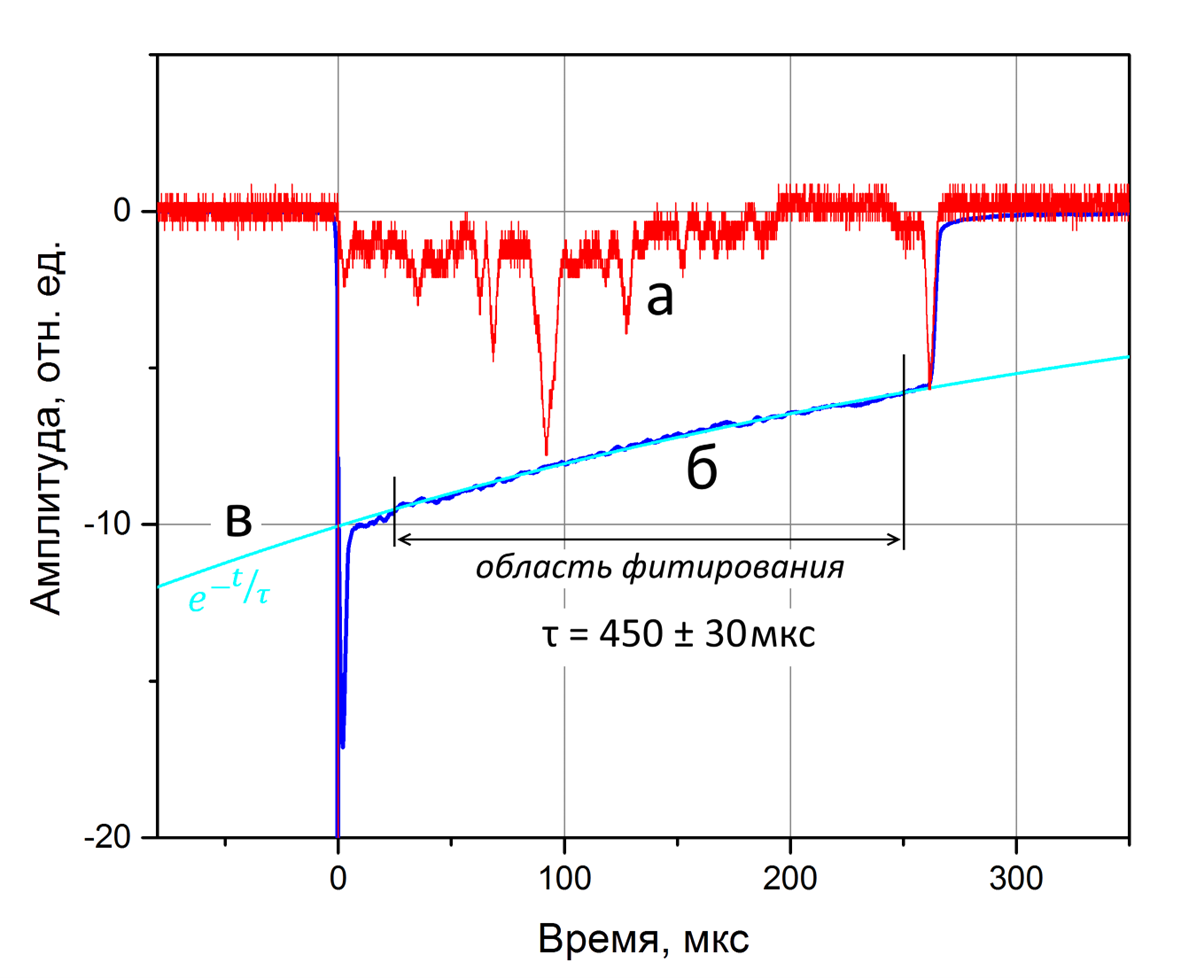
\includegraphics[width=0.8\linewidth]{images/Graph41_labels.png}}
	\caption[Пример определения времени жизни электронов ионизации до захвата электроотрицательными примесями в жидком ксеноне.]{а) — типичный мюонный сигнал, б) — сигнал, усреднённый по 10 000 событий, в — экспоненциально спадающая функция, аппроксимирующая «ступеньку» усреднённого сигнала.}
	\label{img:muonsignal}
\end{figure}

Эволюция времени жизни в течение сеанса показана
на рисунках \ref{img:lt2019}, \ref{img:lt2022}

\begin{figure}[H]	\center{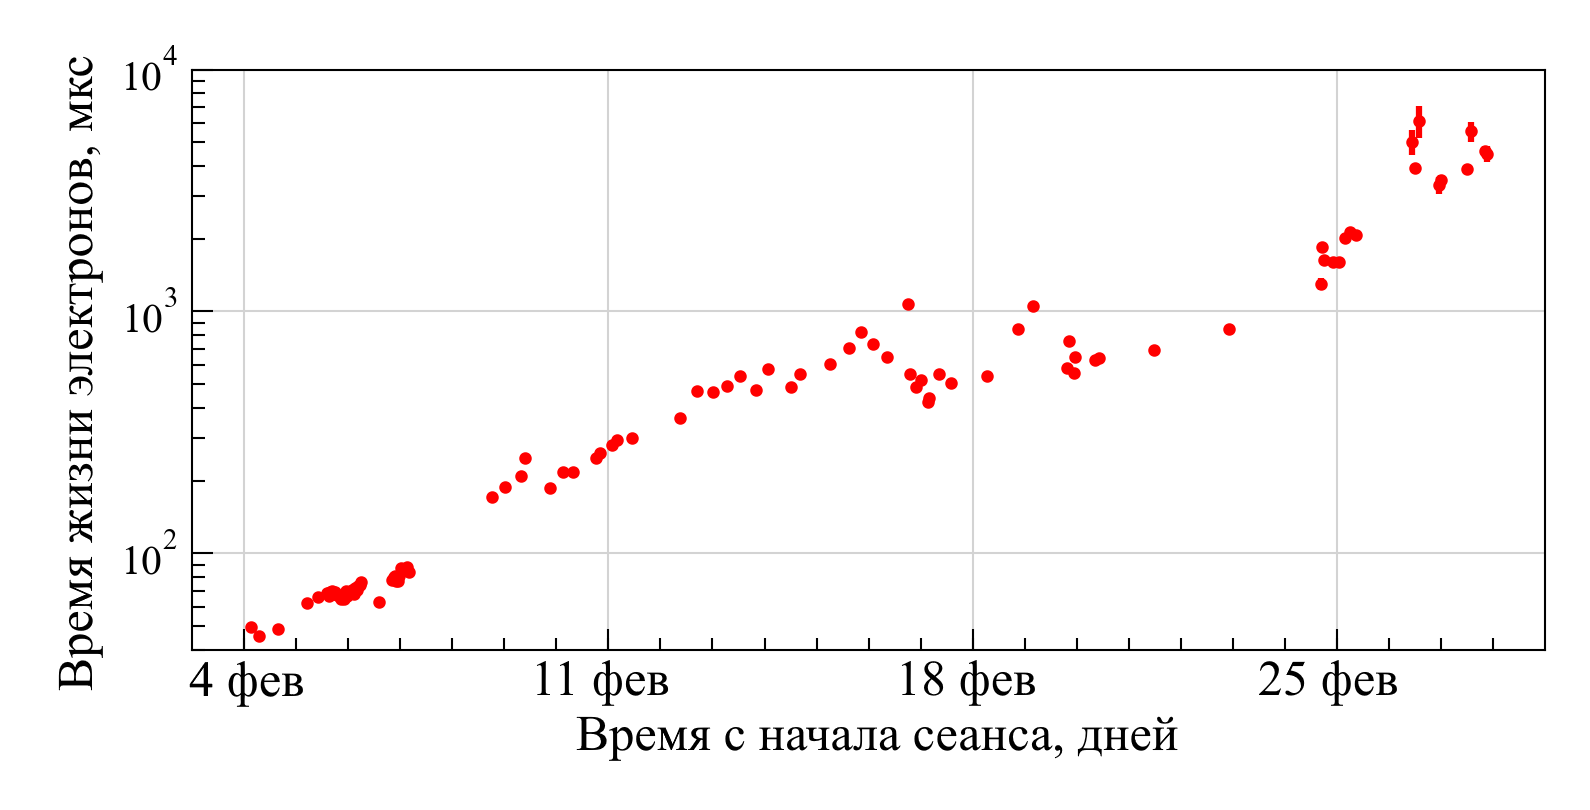
\includegraphics[width=0.8\linewidth]{images/RED100. Graph. e_lifetime_2019_published_RU.png}}
	\caption{Динамика изменения времени жизни электронов в детекторе РЭД-100 в течение инженерного сеанса 2019 года}
	\label{img:lt2019}
\end{figure}

\begin{figure}[H]	\center{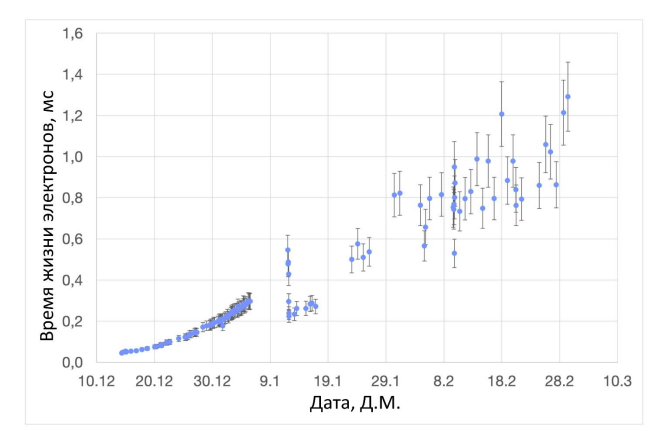
\includegraphics[width=0.8\linewidth]{images/lifetime2022.png}}
	\caption{Динамика изменения времени жизни электронов в детекторе РЭД-100 в течение сеанса на КАЭС 2022 года}
	\label{img:lt2022}
\end{figure}

%Как вы можете видеть, достигнута хорошая чистота, которая соответствует на полной длине дрейфа не больше чем ... (процент от сигнала).
%+ мб про концентрацию? (Леше задать вопрос)

\section{LED-калибровка}
\label{sect3_2}
После обработки данных пакетом REDOffline, из обнаруженных импульсов отбирались импульсы с амплитудой и длительностью больше пороговых, которые представлены в таблице \ref{tab:spethresholds}.
\begin{table}[hbt]
    \centering
        \caption{Пороговые значения для отбора импульсов с целью получения спектров SPE сигналов.}
\begin{tabular}{|c|c|c|}
\hline
    Сеанс & Амплитуда & Длительность\\
    \hline
    2019 & 1.5 мВ & 4 нс\\
    \hline
    2021-22 & 2 мВ & 4 нс\\
    \hline
\end{tabular}
    \label{tab:spethresholds}
\end{table}

Характерные значения зарядов однофотоэлектронных сигналов ФЭУ были получены на основе фитирования спектров площадей отобранных импульсов следующей функцией:
%переназвать N ()
\begin{equation}
N=\exp (a+k Q)+c \cdot \exp \left(-\frac{\left(Q-Q_0\right)^2}{2 \sigma^2}\right)
\label{spefitfunc}
\end{equation}
\par В данной формуле $Q$ - площадь (заряд) импульса ФЭУ,  Экспоненциальное слагаемое в данном случае соответствует шумовой части спектра, а распределение Гаусса -- непосредственно спектру однофотоэлектронных сигналов. Результат 2019 года показал, что интересующий нас сигнал отстоит достаточно далеко от шумов электроники, поэтому при анализе данных, набранных на КАЭС фитирование производилось только распределением Гаусса. Примеры фитированных спектров представлены на рисунке \ref{img:spe2019} для 2019 года и на рисунке \ref{img:spe2022} для 2021-22. 

\begin{figure}[H]
	\center{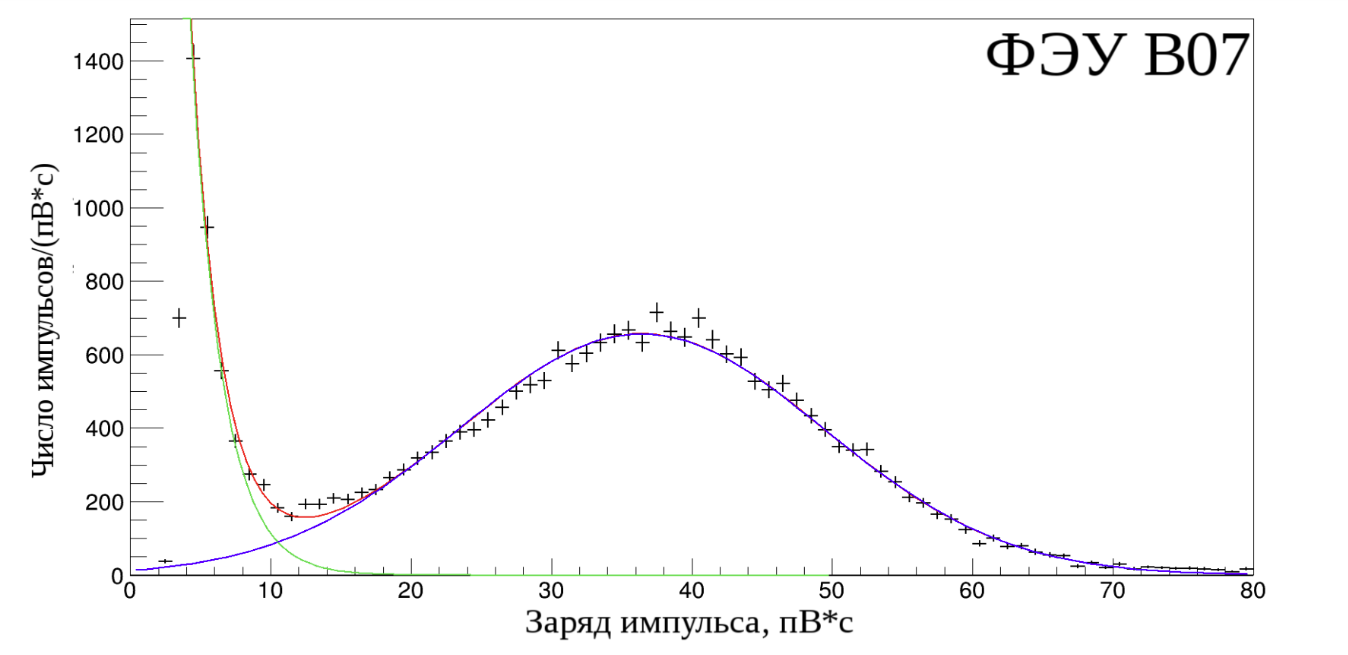
\includegraphics[width=0.8\linewidth]{images/SPE_spectrum.png}}
	\caption[Спектр площадей импульсов для ФЭУ В07(из нижней матрицы) и результат его фитирования функцией \ref{spefitfunc}) для инженерного запуска РЭД-100.] {Спектр площадей импульсов для ФЭУ В07(из нижней матрицы) и результат его фитирования функцией \ref{spefitfunc}) для инженерного запуска РЭД-100. Синим обозначена часть, соответствующая нормальному распределению, зеленым -- часть, соответствующая экспоненциальной функции, красным -- их сумма.}
	\label{img:spe2019}
\end{figure}

\begin{figure}[H]
	\center{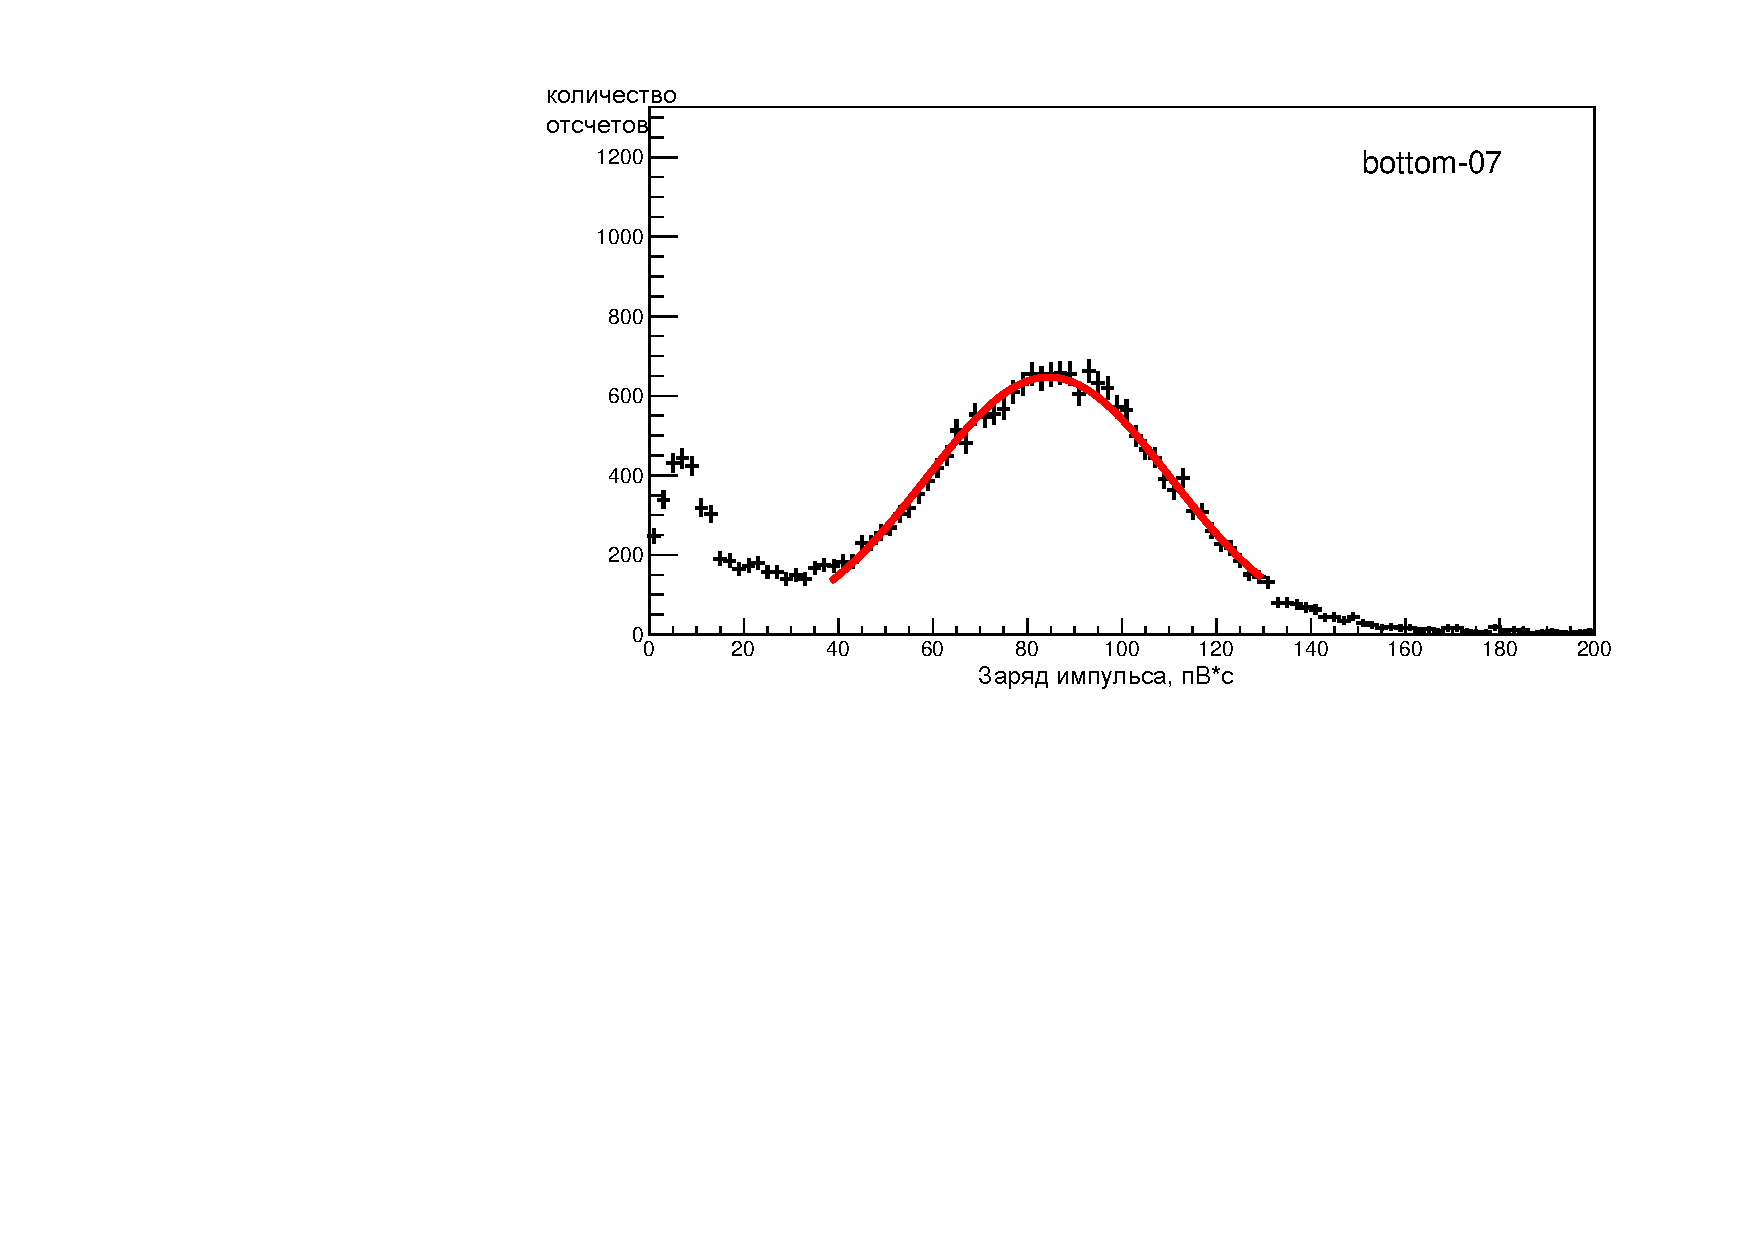
\includegraphics[width=0.8\linewidth]{images/ledspectrum2022.pdf}}
	\caption[Спектр площадей импульсов для ФЭУ В07(из нижней матрицы) и результат его фитирования распределением Гаусса для эксперимента на КАЭС.]{Спектр площадей импульсов для нескольких ФЭУ и результат фитирования распределением Гаусса для эксперимента на КАЭС. Красной линией обозначен результат фитирования.}
	\label{img:spe2022}
\end{figure}

Результаты SPE-калибровок с использованием светодиода для инженерного сеанса и сеанса на КАЭС для всех ФЭУ приведены в таблицах в~\ref{AppendixA1}. Существенное (более чем в два раза) отличие характерных зарядов SPE для двух сеансов связано с изменением рабочего напряжения на ФЭУ. 

Сеанс набора данных на КАЭС был существенно дольше, чем инженерный ран в МИФИ, поэтому требовался более тщательный анализ SPE-калибровок. Для дополнительной проверки помимо импульсов из данных, набранных со светодиодом, были отобраны одиночные импульсы на формах сигналов от SE-калибровок, а также на формах сигналов с УКРН-подобными событиями. Пример сравнения полученных положений SPE пика представлен на рисунке \ref{img:spevstime2022}. 

\begin{figure}[H]
	\center{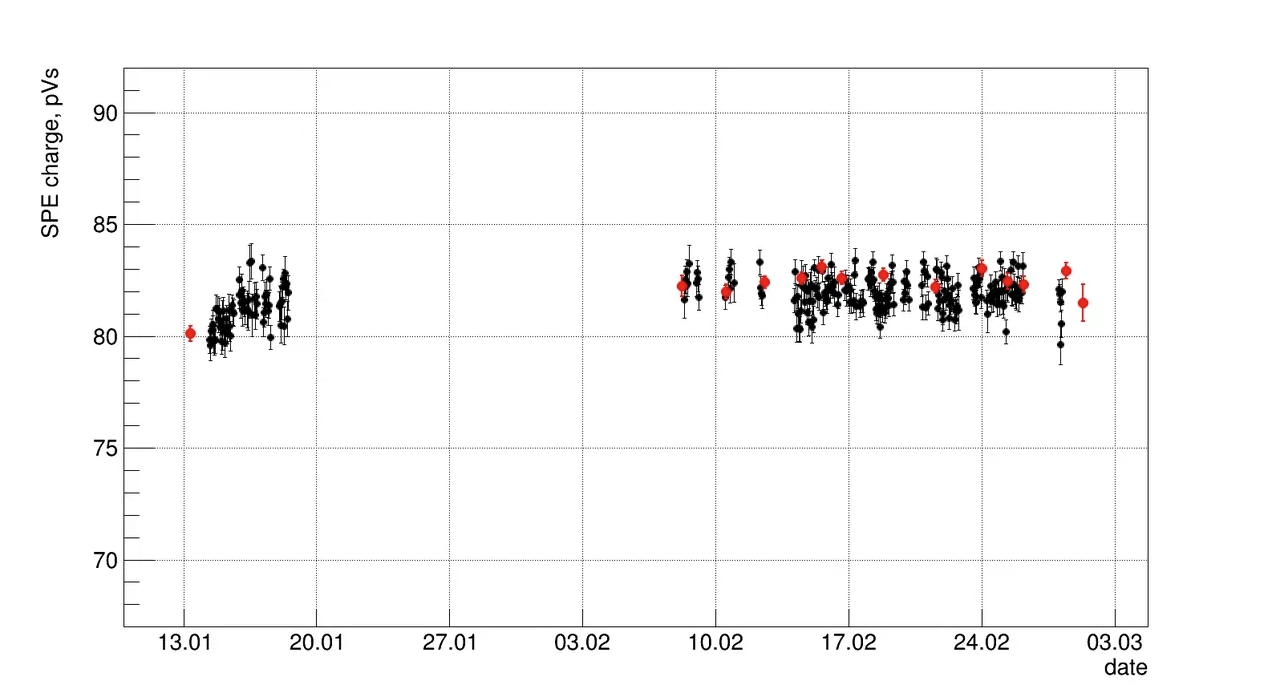
\includegraphics[width=0.8\linewidth]{images/spevstime2022.png}}
	\caption[Пример зависимости положения SPE-пика, полученного разными способами, от времени.] {Пример зависимости положения SPE-пика, полученного разными способами, от времени. Черным обозначены измерения при помощи SE калибровок, красным -- при помощи LED калибровок. Промежуток в наборе данных связан с техническими неполадками.}
	\label{img:spevstime2022}
\end{figure}

Кроме того, так как сеанс набора данных был длительный, была обнаружена слабая зависимость величины SPE импульсов от времени. Она связана с изменением параметров детектора и электроники. Так как измерения на КАЭС требовали повышенной точности, данная зависимость была учтена путем фитирования зависимости данных SPE-калибровок кусочно-линейной функцией. Пример такого фитирования показан на рисунке~\ref{img:spevstimefit}.

\begin{figure}[H]
	\center{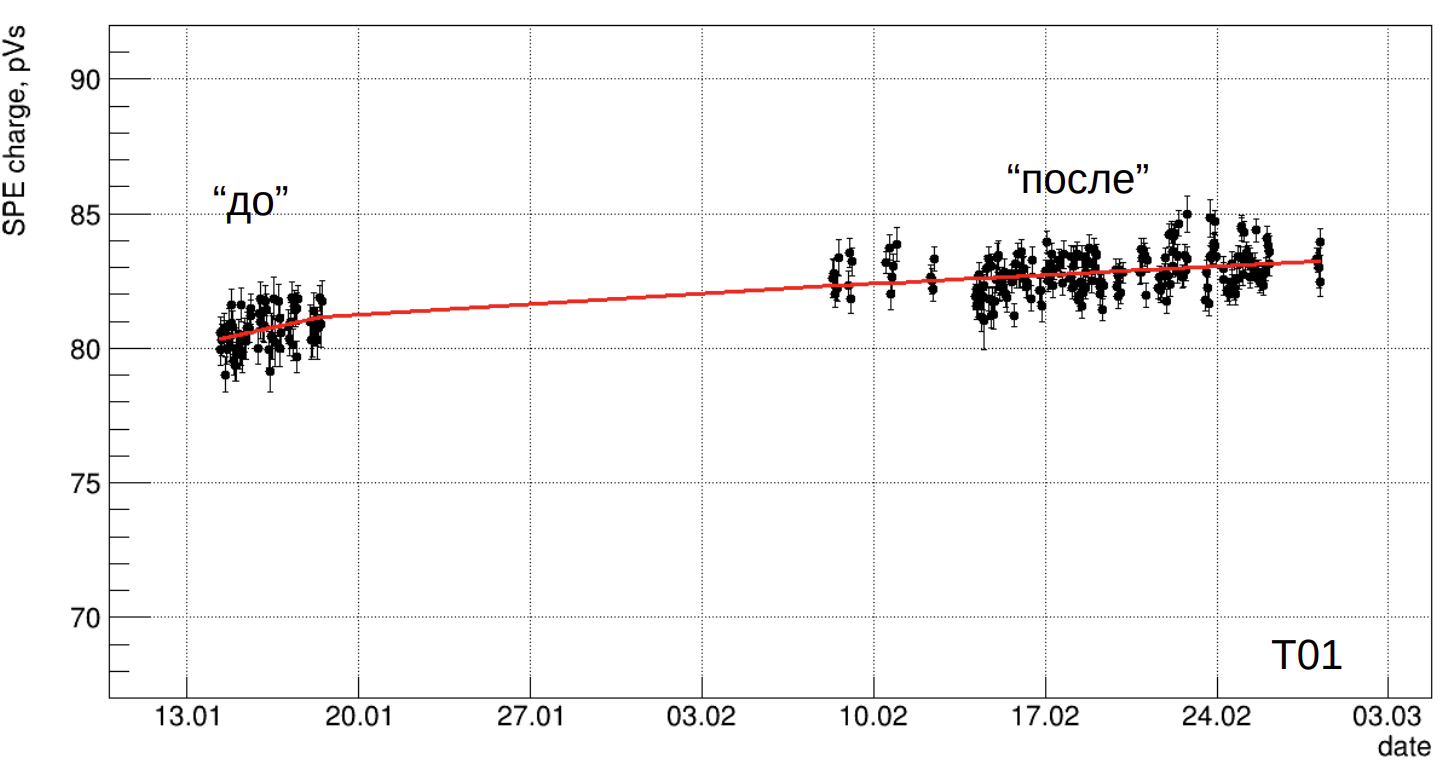
\includegraphics[width=0.8\linewidth]{images/spevstimefit.png}}
	\caption[Пример фитирования зависимости положения SPE пика от времени для ФЭУ Т01.] {Пример фитирования зависимости положения SPE пика от времени кусочно-линейной функцией для ФЭУ Т01. Промежуток в наборе данных связан с техническими неполадками.}
	\label{img:spevstimefit}
\end{figure}

\section{Калибровка гамма-источниками}
\label{sect3_3}
Обработка LED-калибровок предполагает анализ одиночных форм сигналов и выделение на них импульсов соответствующих определенным параметрам. Обработка измерений с гамма-источниками принципиально отличается, так как требует выделений событий, которые которые представляют собой совпадение по времени импульсов во многих каналах и анализа сигналов с разных каналов в комплексе. Для этой цели была разработана цепочка алгоритмов, изложенная в данном разделе.
\subsection{Кластеризация}
\label{subsect3_3_1}
Гамма-кванты дают световыход в детекторе, достаточно большой для того, чтобы в каждом ФЭУ был ощутимый световой сигнал. Поэтому для анализа применяется суммарная форма сигнала, в которой импульсы от физических сигналов в разных ФЭУ будут складываться, а совпадений случайных импульсов с таковыми в других ФЭУ не будет.

После обработки сырых форм сигналов при помощи RED-offline требовалось выделить на них кластеры -- группы импульсов, соответствующие сигналам от сцинтилляции и электролюминесценции. Для ускорения процесса обработки был реализован следующий алгоритм:
\begin{enumerate}
    \item Формировались прямоугольные импульсы, длительность которых была равна длительности оригинального импульса, а высота определялась как отношение площади оригинального импульса к его длительности
    \item Полученные прямоугольные импульсы со всех каналов складывались в одну суммарную псевдо-форму сигнала
    \item На полученной псевдо-форме сигнала проводился поиск импульсов, соответствующих S1 и S2 по следующим критериям:
    \begin{itemize}
        \item S1: длительность от 70 нс до 170 нс; амплитуда от 0.4e-6 В до 1.8e-6 В 
        \item S2: длительность больше 1800 нс; по амплитуде дополнительных отборов не применялось.
    \end{itemize}
\end{enumerate}
Из оригинальных импульсов, содержащихся в отобранных кластерах, формировались калибровочные события. Площадь каждого сигнала S2 была скорректирована в соответствии с временем жизни электронов в жидком ксеноне. Также площади, изначально определенные в В$\cdot$с, были поделены на площади единичного SPE для каждого ФЭУ. 
Также был произведен переход от измерения площадей в В$\cdot$с к измерению в единицых SPE, что позволило избавиться от эффектов зависимости SPE-калибровок от времени и номера канала.

Для дальнейшего анализа был применен дополнительный отбор на количество S1 и S2 -- каждое событие должно было содержать ровно одну вспышку S1 и одну S2. Данный отбор необходим для более чистого разделения событий и выделения калибровочных пиков.

\subsection{Пространственное восстановление}
\label{subsect3_3_2}
Наиболее простым способом получения координат событий является центроид, который состоит в том, что координата вспышки находится по формуле~\cite{6154607}:
\begin{equation}
    X_{event} = \frac{\sum\limits_{i}A_iX_i}{\sum\limits_{i}A_i},
\end{equation}
где $X_i$, $A_i$ --- координаты и сигналы ФЭУ в данном событии. Энергия в данном случае может быть восстановлена как простая сумма сигналов. Здесь и далее под сигналом ФЭУ понимается площадь импульсов. Однако, данный метод позволяет эффективно восстанавливать координаты событий только в непосредственной близости от центра детектора. События, которые произошли по краям рабочего объема, при восстановлении центроидом стягиваются ближе к центру (рисунок \ref{ris:basecen}), так как сигнал с центральных ФЭУ ничем не компенсируется для краевых событий. Несомненным плюсом восстановления методом центроида является отсутствие необходимости в каких-либо других данных и расчетах кроме откликов ФЭУ и их координат.
\begin{figure}[hbt]
	\center{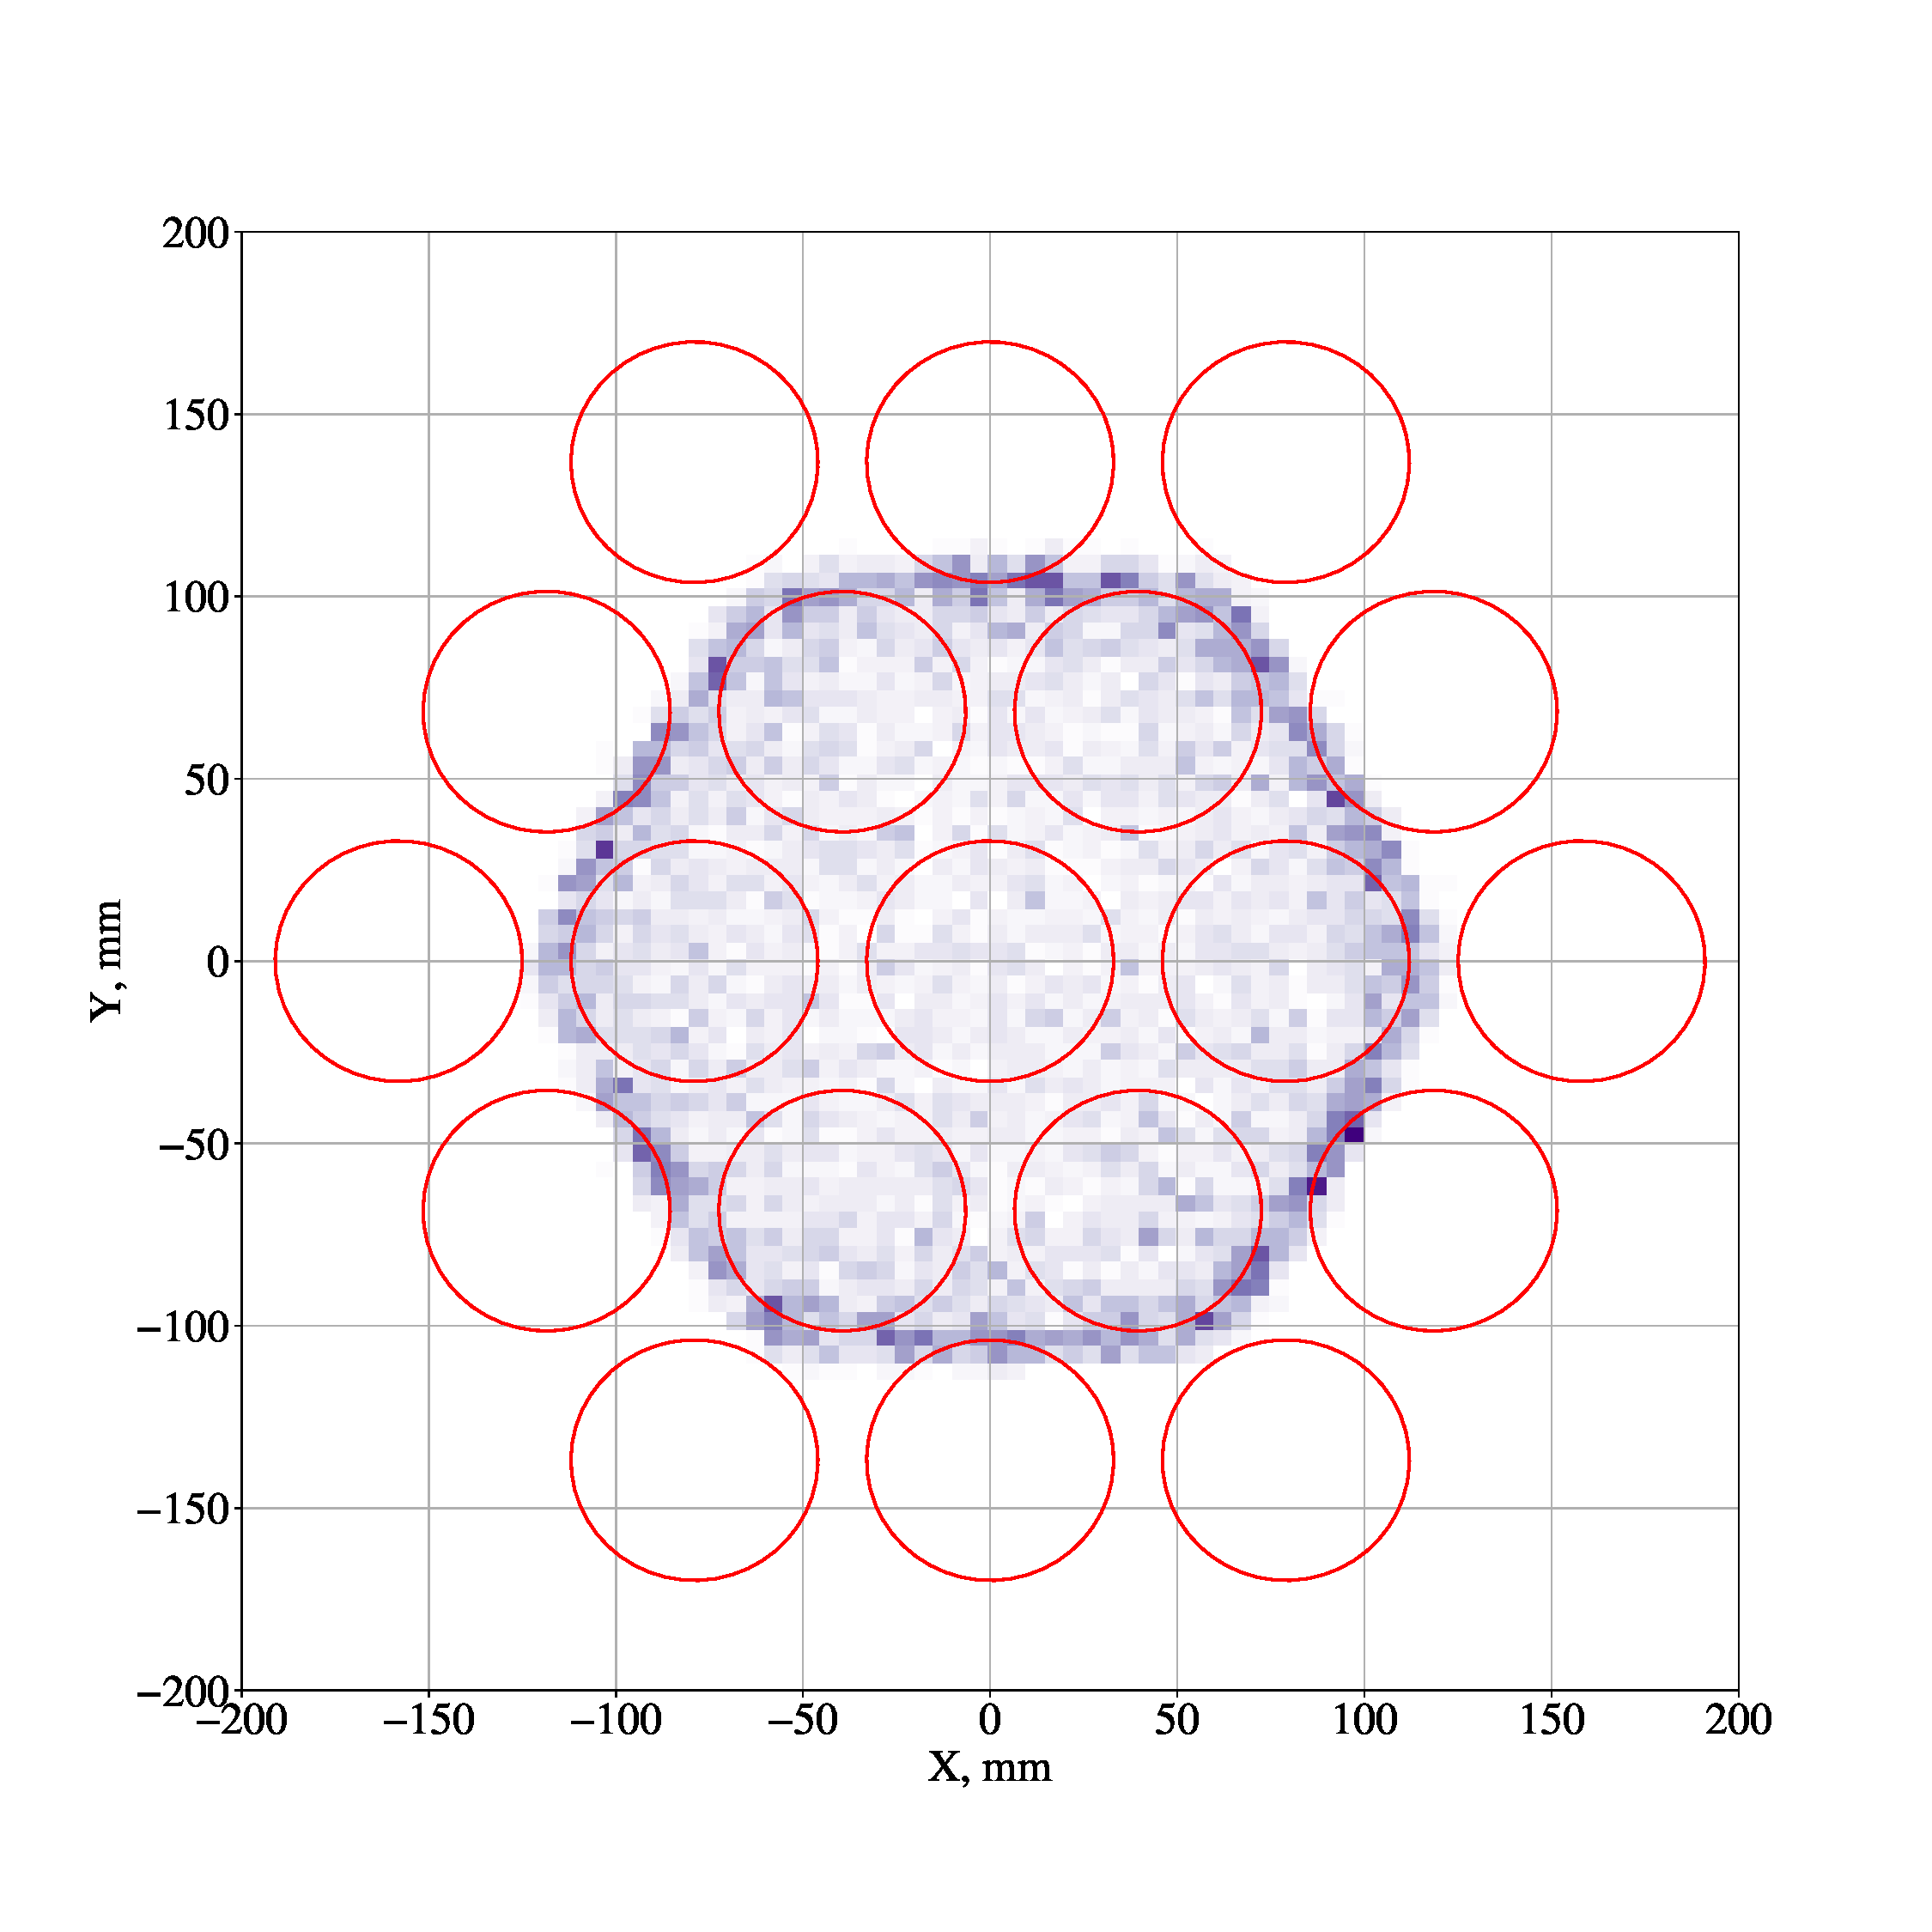
\includegraphics[width=0.8\linewidth]{images/basecentro.pdf}}
	\caption{Распределение восстановленных смоделированных событий методом нескорректированного центроида. Красными окружностями обозначены ФЭУ.}
	\label{ris:basecen}
\end{figure}
%развернуть этот график
\begin{figure}[hbt]
	\center{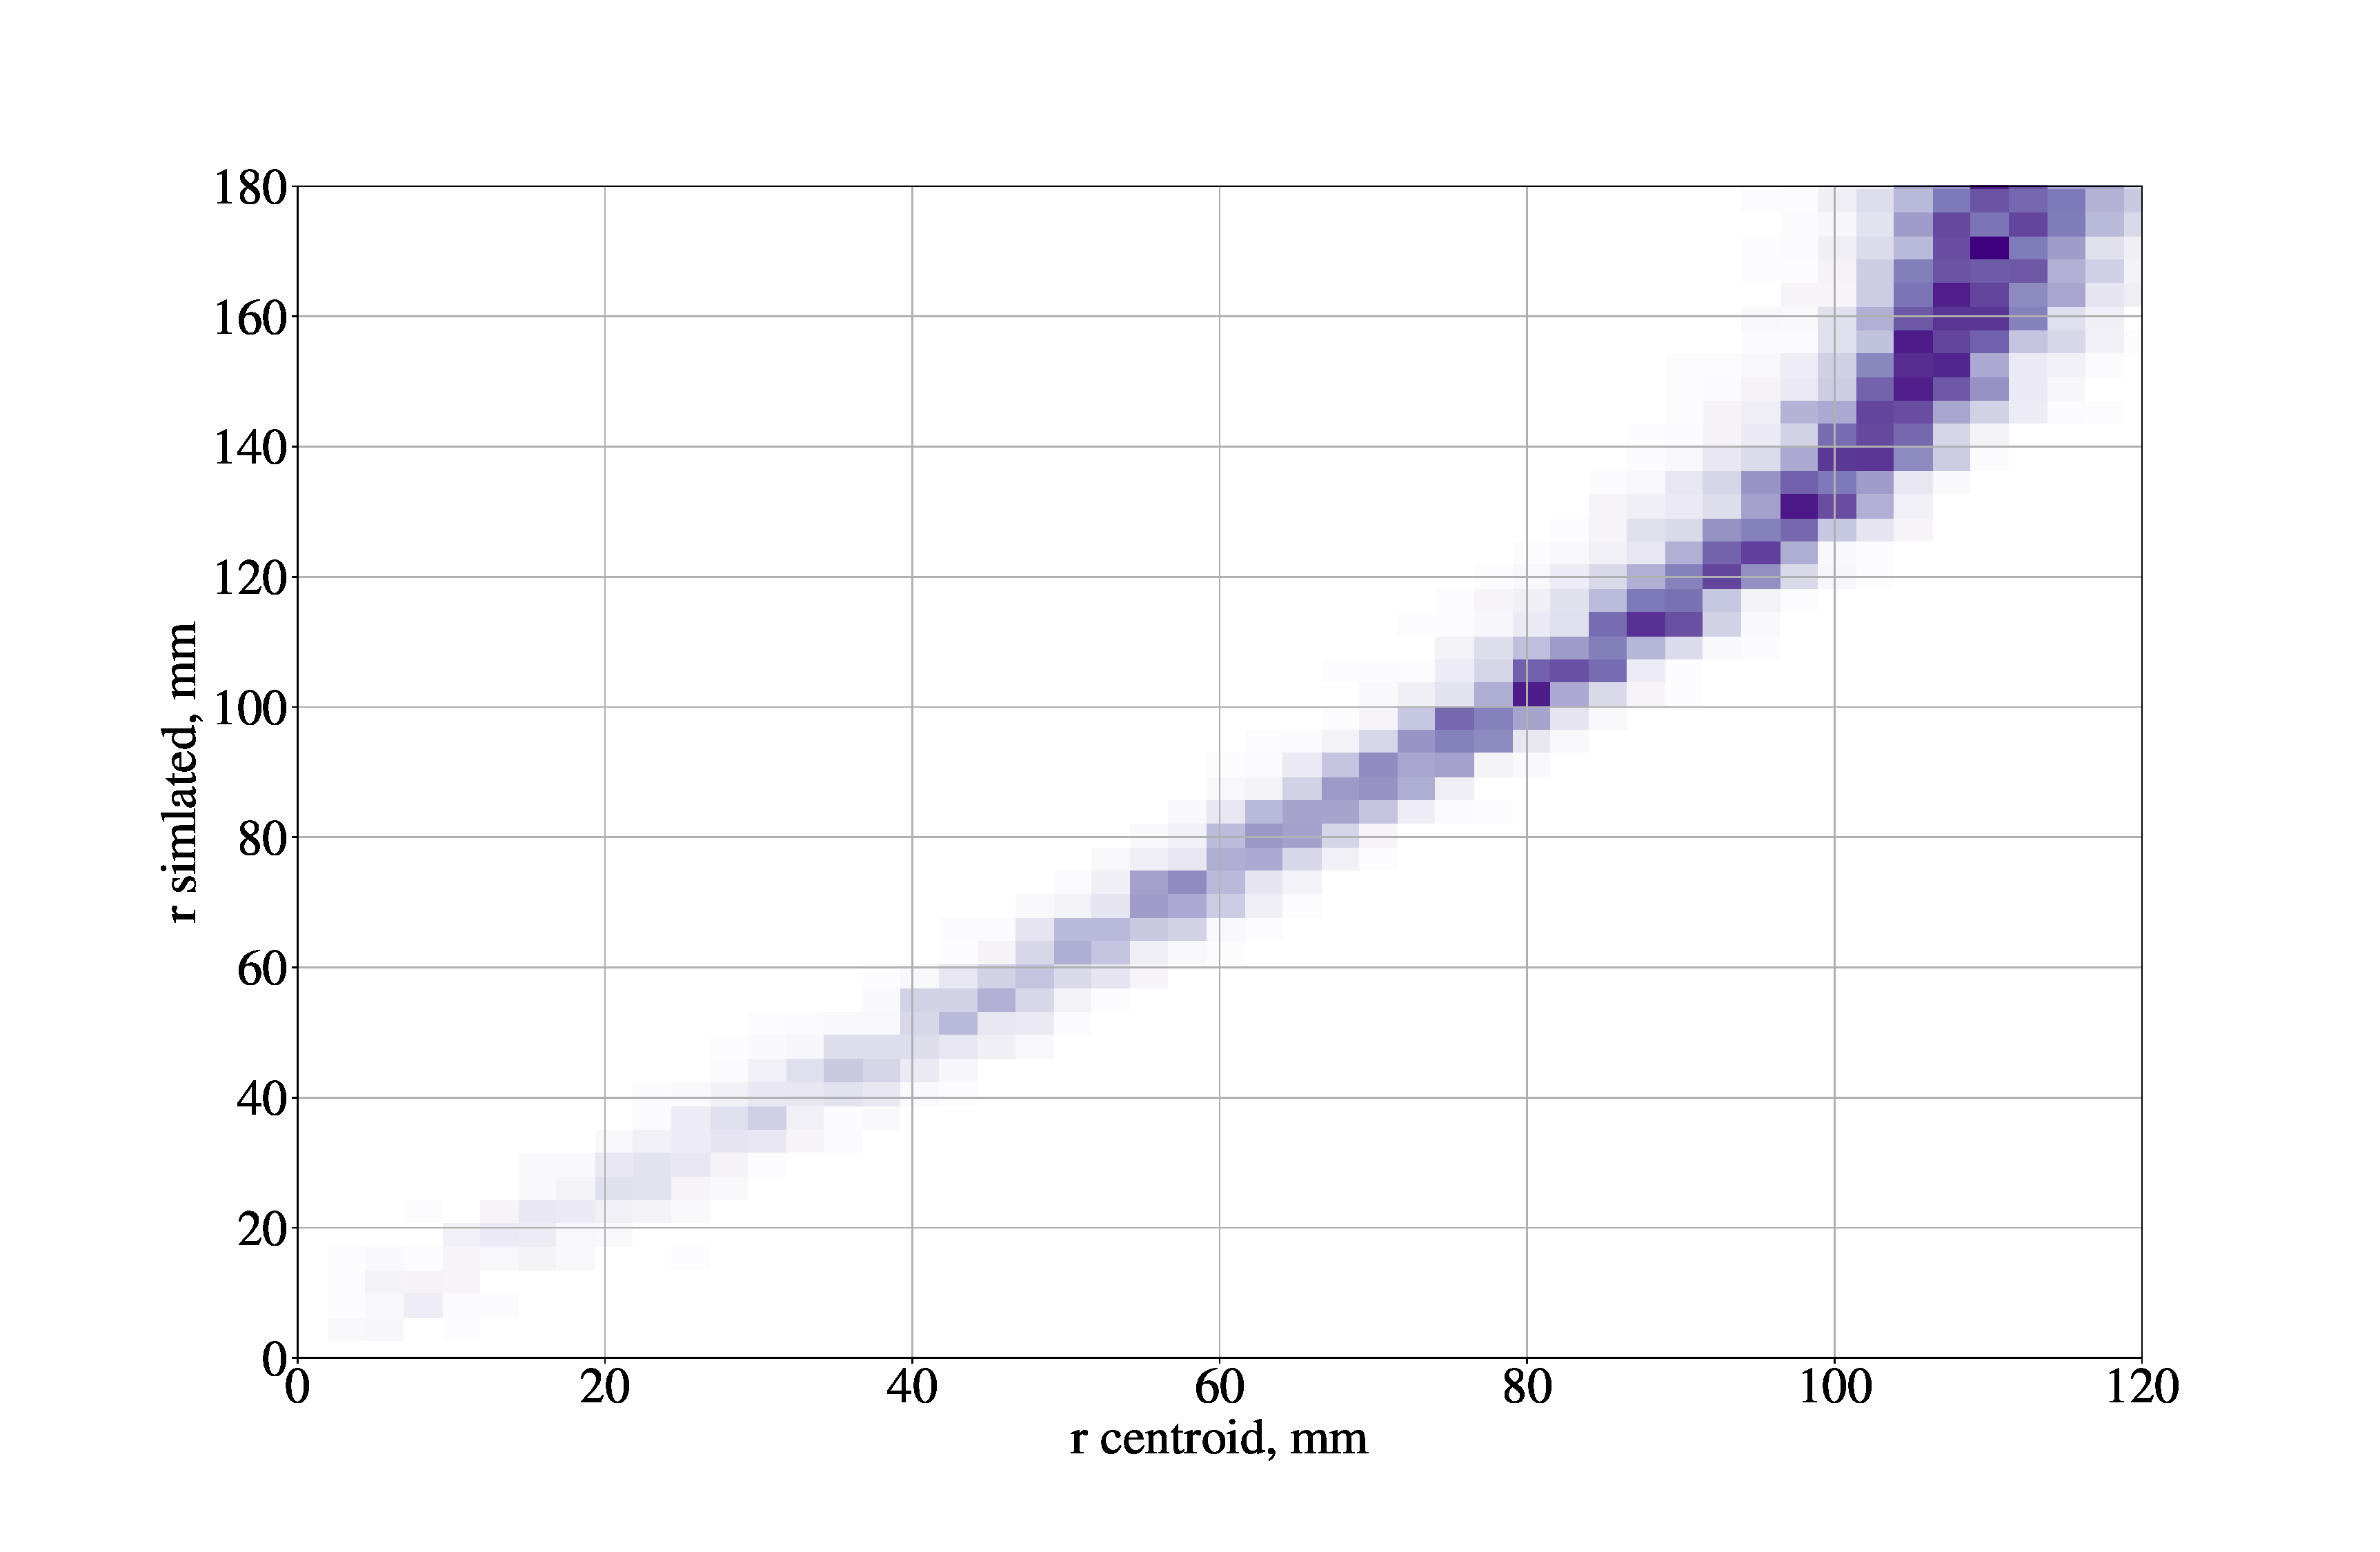
\includegraphics[width=1\linewidth]{images/rvsr.pdf}}
	\caption{Зависимость радиуса для смоделированных событий от радиуса, полученного в результате восстановления методом центроида}
	\label{ris:rvsr}
\end{figure}
\parИдея многих других методов пространственного восстановления заключается в построении функций эффективности светосбора (light response functions --- LRF) для каждого ФЭУ, которая представляет собой зависимость отклика ФЭУ от положения источника света. Эти методы опираются на предположение, что форма LRF не зависит от количества света, что с высокой степенью надежности выполняется в большинстве случаев. Формы LRF могут быть получены разными способами, как аналитическим расчетом, так и в результате моделирования или анализа экспериментальных данных, а также комбинацией этих способов. Наиболее простой метод, основанный на использовании LRF --- скорректированный центроид. В данном случае удобнее использовать полярные координаты $r$ и $\varphi$. На рисунке~\ref{ris:rvsr} приведена зависимость полярного радиуса для некоторых смоделированных событий от радиуса, полученного в результате восстановления координат этих событий методом центроида. С использованием данной зависимости производится поиск функции $r_{corrcentr} = f(r_{centr}, \varphi)$, где $r_{corrcentr}$, $r_{centr}$ --- скорректированный и нескорректированный радиус.  Искажения полярного угла $\varphi$ обычно малы и его коррекция может не производиться. Для детектора РЭД-100 один из вариантов вида функции $f$, определенный эмпирическим путем, выглядит следующим образом:
\begin{equation}
   f(r_{centr}, \varphi) = \Big(A\cdot r_{centr}^2+B\cdot r_{centr}\Big)\cdot\Big( 1-C\cdot \exp(D\cdot r_{centr})\cdot(\cos 6\varphi)\Big),
\end{equation}
где $A, B, C, D$ --- параметры, вычисляемые исходя из имеющихся LRF. Данный метод не обеспечивает высокой точности восстановления, однако отличается своей быстротой и простотой применения.
\par Более сложными и затратными, но одновременно и более точными являются метод максимального правдоподобия с учетом LRF и статистики фотонов~\cite{6154607}, который и был использован в данной работе. Минимизация проводилась методом сжимающихся сеток~\cite{grids}, описанным далее. Область вокруг некоторой стартовой координаты разбивается на сетку с определенным шагом. В каждом узле рассчитывается правдоподобие между ожидаемым и наблюдаемым откликом ФЭУ в данной точке. Ищется узел с максимальным значение функции правдоподобием. Данный узел на следующей итерации принимается за стартовое положение, вокруг которого строится сетка уже с меньшим шагом. 
Визуализация данного метода представлена на рисунке~\ref{ris:grids}.
\begin{figure}[hbt]
	\center{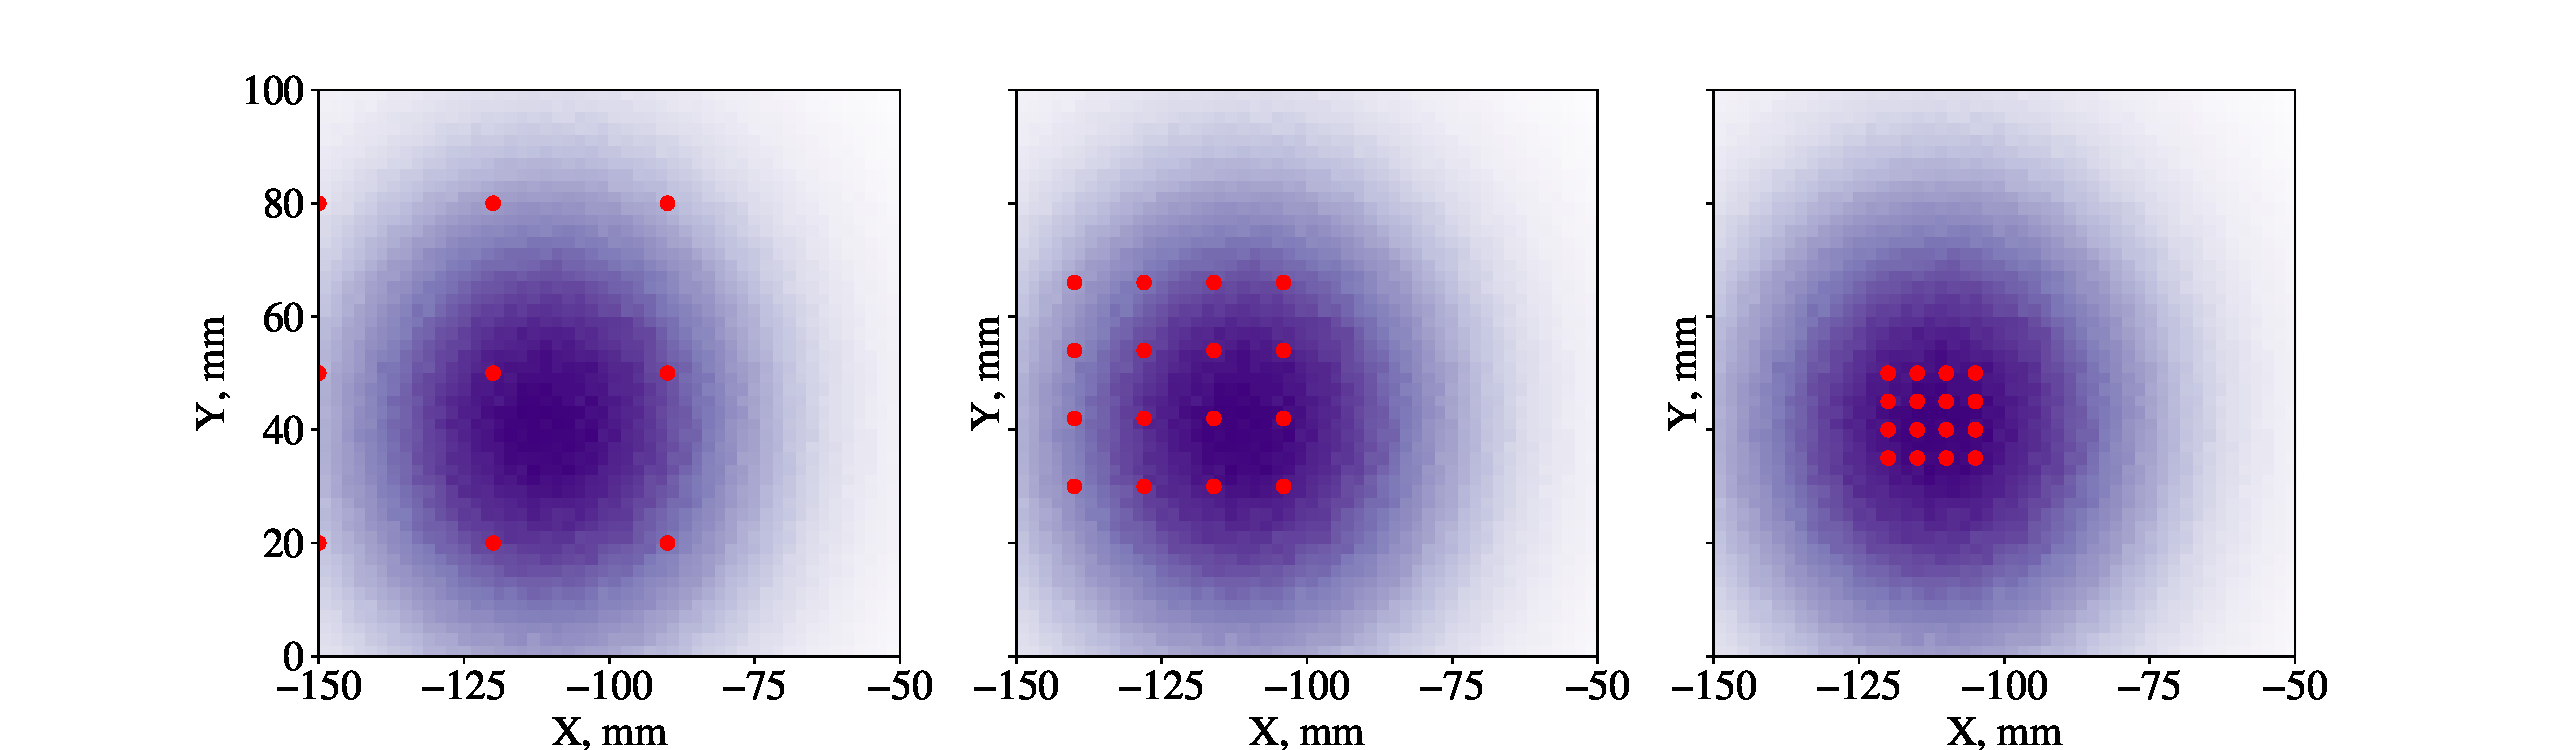
\includegraphics[width=1\linewidth]{images/grids.pdf}}
	\caption{Визуализация метода сжимающихся сеток}
	\label{ris:grids}
\end{figure}
На каждой итерации при минимизации производится восстановление энергии. Энергия определялась как отношение суммы сигналов со всех ФЭУ и суммы значений LRF в точке с восстановленными координатами.
\\
\par\textbf{Использование калибровочных данных для восстановления формы LRF}
\par
Как уже упоминалось, гамма-кванты, излучаемые использованными калибровочными источниками, имеют большую энергию, достаточную для засвечивания всей верхней матрицы детектора. Это позволяет определять LRF по калибровочным данным и использовать их в дальнейшем при обработке,  в том числе для событий с существенно меньшей энергией. Построение LRF производилось итеративно в соответствии с методикой из~\cite{6154607}  описанным далее способом (схема алгоритма приведена на рисунке~\ref{ris:lrfscheme}). 
\begin{figure}[hbt]
	\center{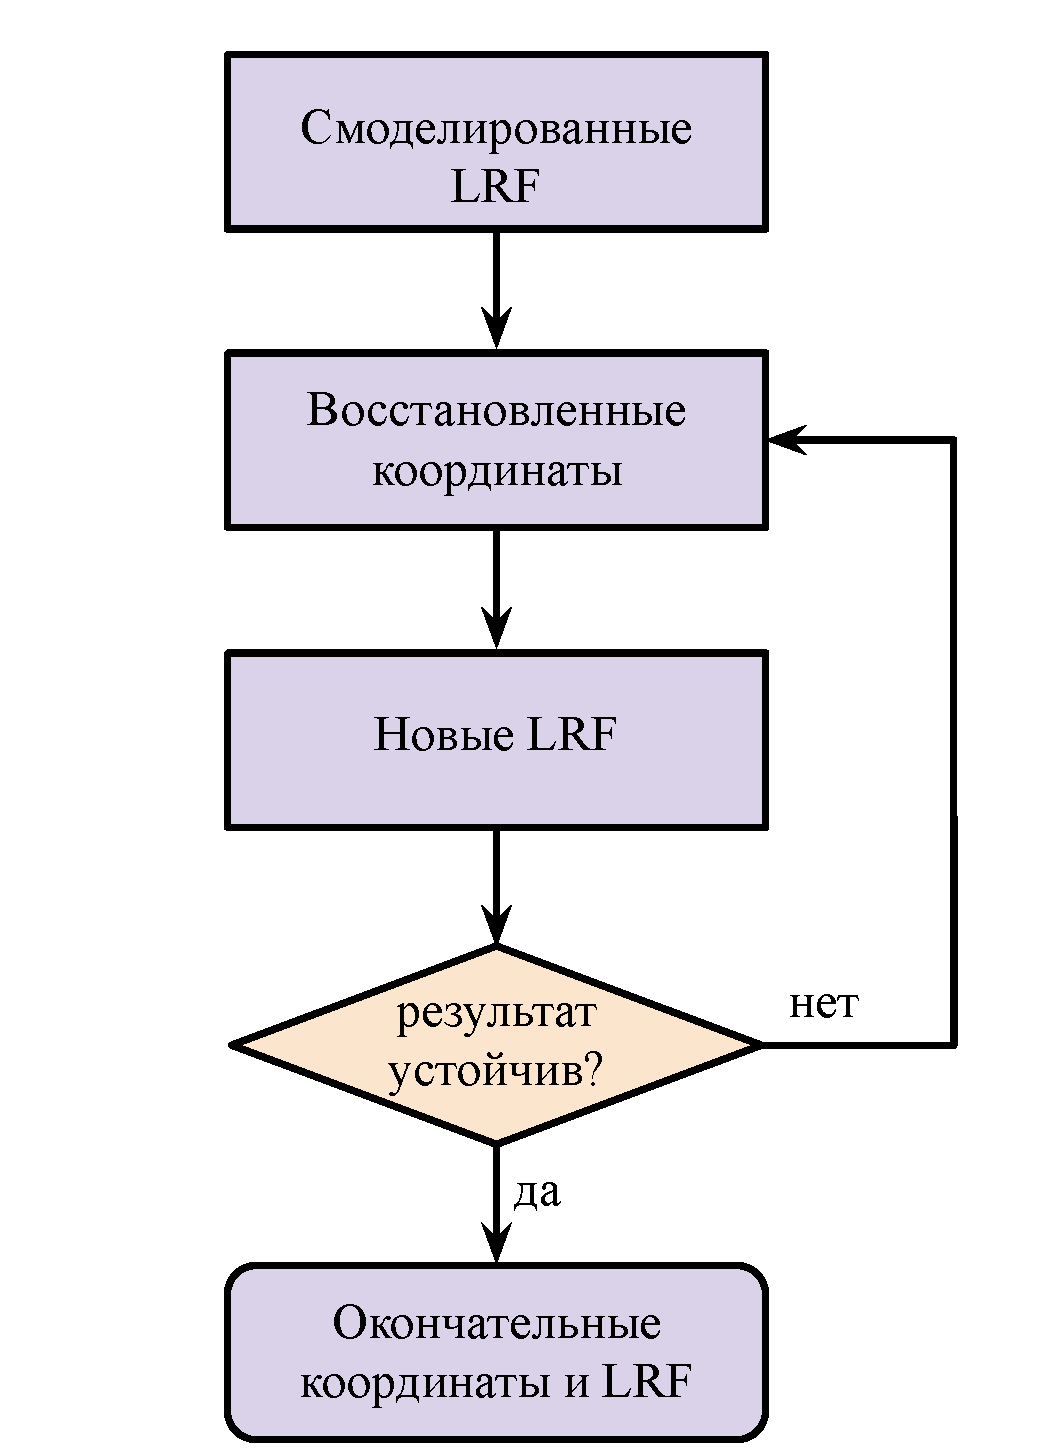
\includegraphics[width=0.6\linewidth]{scheme.pdf}}
	\caption{Алгоритм восстановления координат и LRF}
	\label{ris:lrfscheme}
\end{figure}
Производилось восстановление событий по имеющимся LRF, при этом в качестве начального приближения использовались LRF, построенные в результате моделирования. На основании полученных положений событий и энергии строились новые LRF, а затем новые положения. В качестве стартовых координат при минимизации были выбраны координаты ФЭУ с максимальным откликом в данном событии. При построении LRF не учитывались события, при восстановлении оказавшиеся за пределами детектора. Кроме того, На LRF накладывались следующие ограничения из физических соображений:
\begin{itemize}
    \item функция должна была монотонно убывать с увеличением r;
    \itemв точке $r = 0$ требовалось равенство нулю первой производной по $r$; 
    \itemфункция должна была быть неотрицательна.
\end{itemize}
\parКроме того, для построения LRF ФЭУ группировались в зависимости от расстояния до центра детектора.
Далее опять производилось восстановление координат. Процесс повторялся итеративно до достижения устойчивого результата, что означает, что последующие итерации не приводят к заметным изменениям в восстановленных координатах.

\subsection{Калибровки гамма-источниками во время инженерного сеанса}
\label{subsect3_3_4}
В рамках физических тестов детектора РЭД-100 в ЛЭЯФ НИЯУ МИФИ в 2019 году были набраны данные с использованием калибровочных радиоактивных источников $^{60}$Co и $^{22}$Na. В процессе распада данные элементы излучают гамма-кванты с энергиями 511 кэВ ($^{22}$Na), 1173 кэВ и 1333 кэВ ($^{60}$Co). При наборе данных источники находились на определеной высоте с одной стороны детектора, источник $^{60}$Co был коллимирован, а для набора данных с источником $^{22}$Na была задействована схема совпадений с детектором NaI[Tl] После процедур поиска импульсов и кластеризации для получения LRF были использованы события от $^{60}$Co, на которые были наложены отборы, позволившие отобрать события из пика.
\begin{figure}[hbt]
	\center{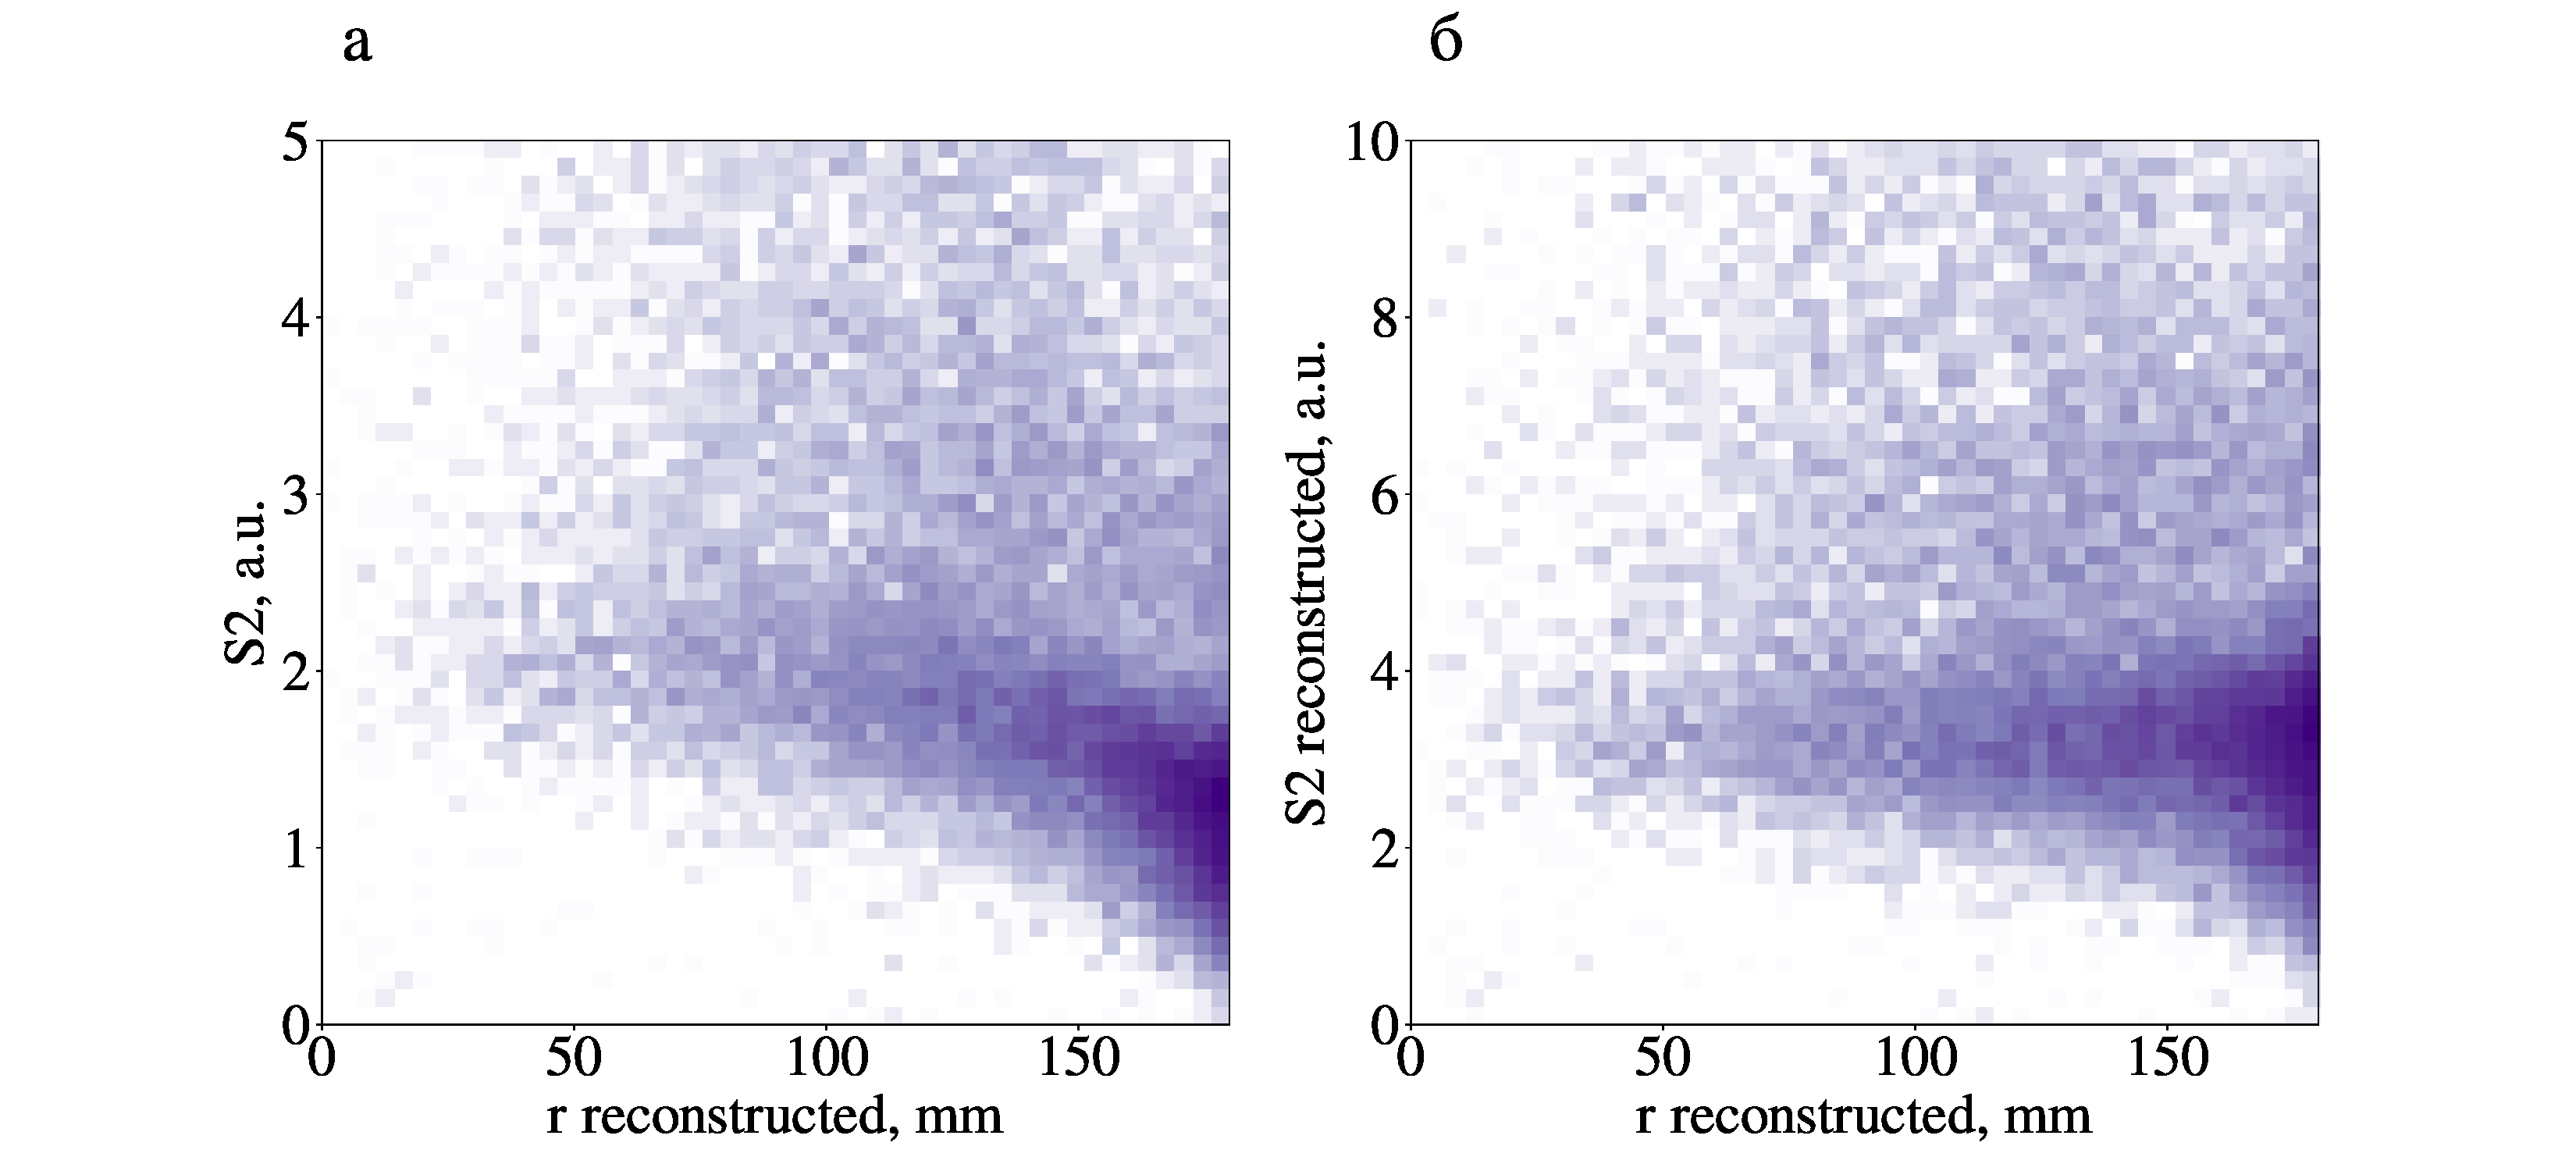
\includegraphics[width=1\linewidth]{energyvsr.pdf}}
	\caption{Зависимость суммарного сигнала(а) и восстановленной энергии S2(б) от восстановленного радиуса}
	\label{img:s2vsR2019}
\end{figure}
\parНа рисунке \ref{img:s2vsR2019}(a) представлена зависимость суммарного (не скорректированного) сигнала от восстановленного радиуса. События ближе к краю детектора дают меньший отклик, чем события в центре за счет краевых эффектов. Энергия, восстановленная при помощи описанного выше алгоритма, не падает с увеличением расстояния от центра детектора (рисунок \ref{img:s2vsR2019}(б)), что косвенно указывает корректность проведенной процедуры восстановления. 

С использование полученных LRF было произведено восстановление координат и энергии для событий от $^{22}$Na. Пространственное распределение событий от источников представлено на рисунке~\ref{img:xyplot2019}.
Распределение событий по S1 и S2 до и после коррекции представлено на рисункax~\ref{img:s1s2na},~\ref{img:s1s2co}. Видно, что после коррекции на распределении для $^{60}$Co становятся различимы линии 1173 кэВ и 1333 кэВ, а для $^{22}$Na --- линия 511 кэВ становится более четкой. Для увеличения соотношения сигнал/шум при построении энергетического спектра на события накладывались ограничения на глубину исходя из известного положения источника, восстановленный полярный угол ($\pi/4$, направленный на источник) и расстояние от центра детектора (<175~мм). На рисунках~\ref{img:s1s2co},~\ref{img:s1s2na} видно, как улучшается разрешение для пика от $^{22}$Na и разрешаются пики от $^{60}$Co после восстановления энергии. Экспериментальный энергетический спектр фитировался одним распределением Гаусса в случае $^{22}$Na и суммой двух распределений Гаусса в случае $^{60}$Co.

Полученный калибровочный график и зависимость энергетического разрешения от энергии представлены на рисунке~\ref{img:calibplot2019}. Линейность калибровочного графика свидетельствует о правильности работы детектора и произведенной обработки данных. Значения положений пиков и энергетического разрешения (отношения среднеквадратичного отклонения ($\sigma$) и ширины на полувысоте (FWHM) к положению пиков) также приведены в таблице~\ref{tab:resolution2019}. 

\begin{figure}[H]
	\center{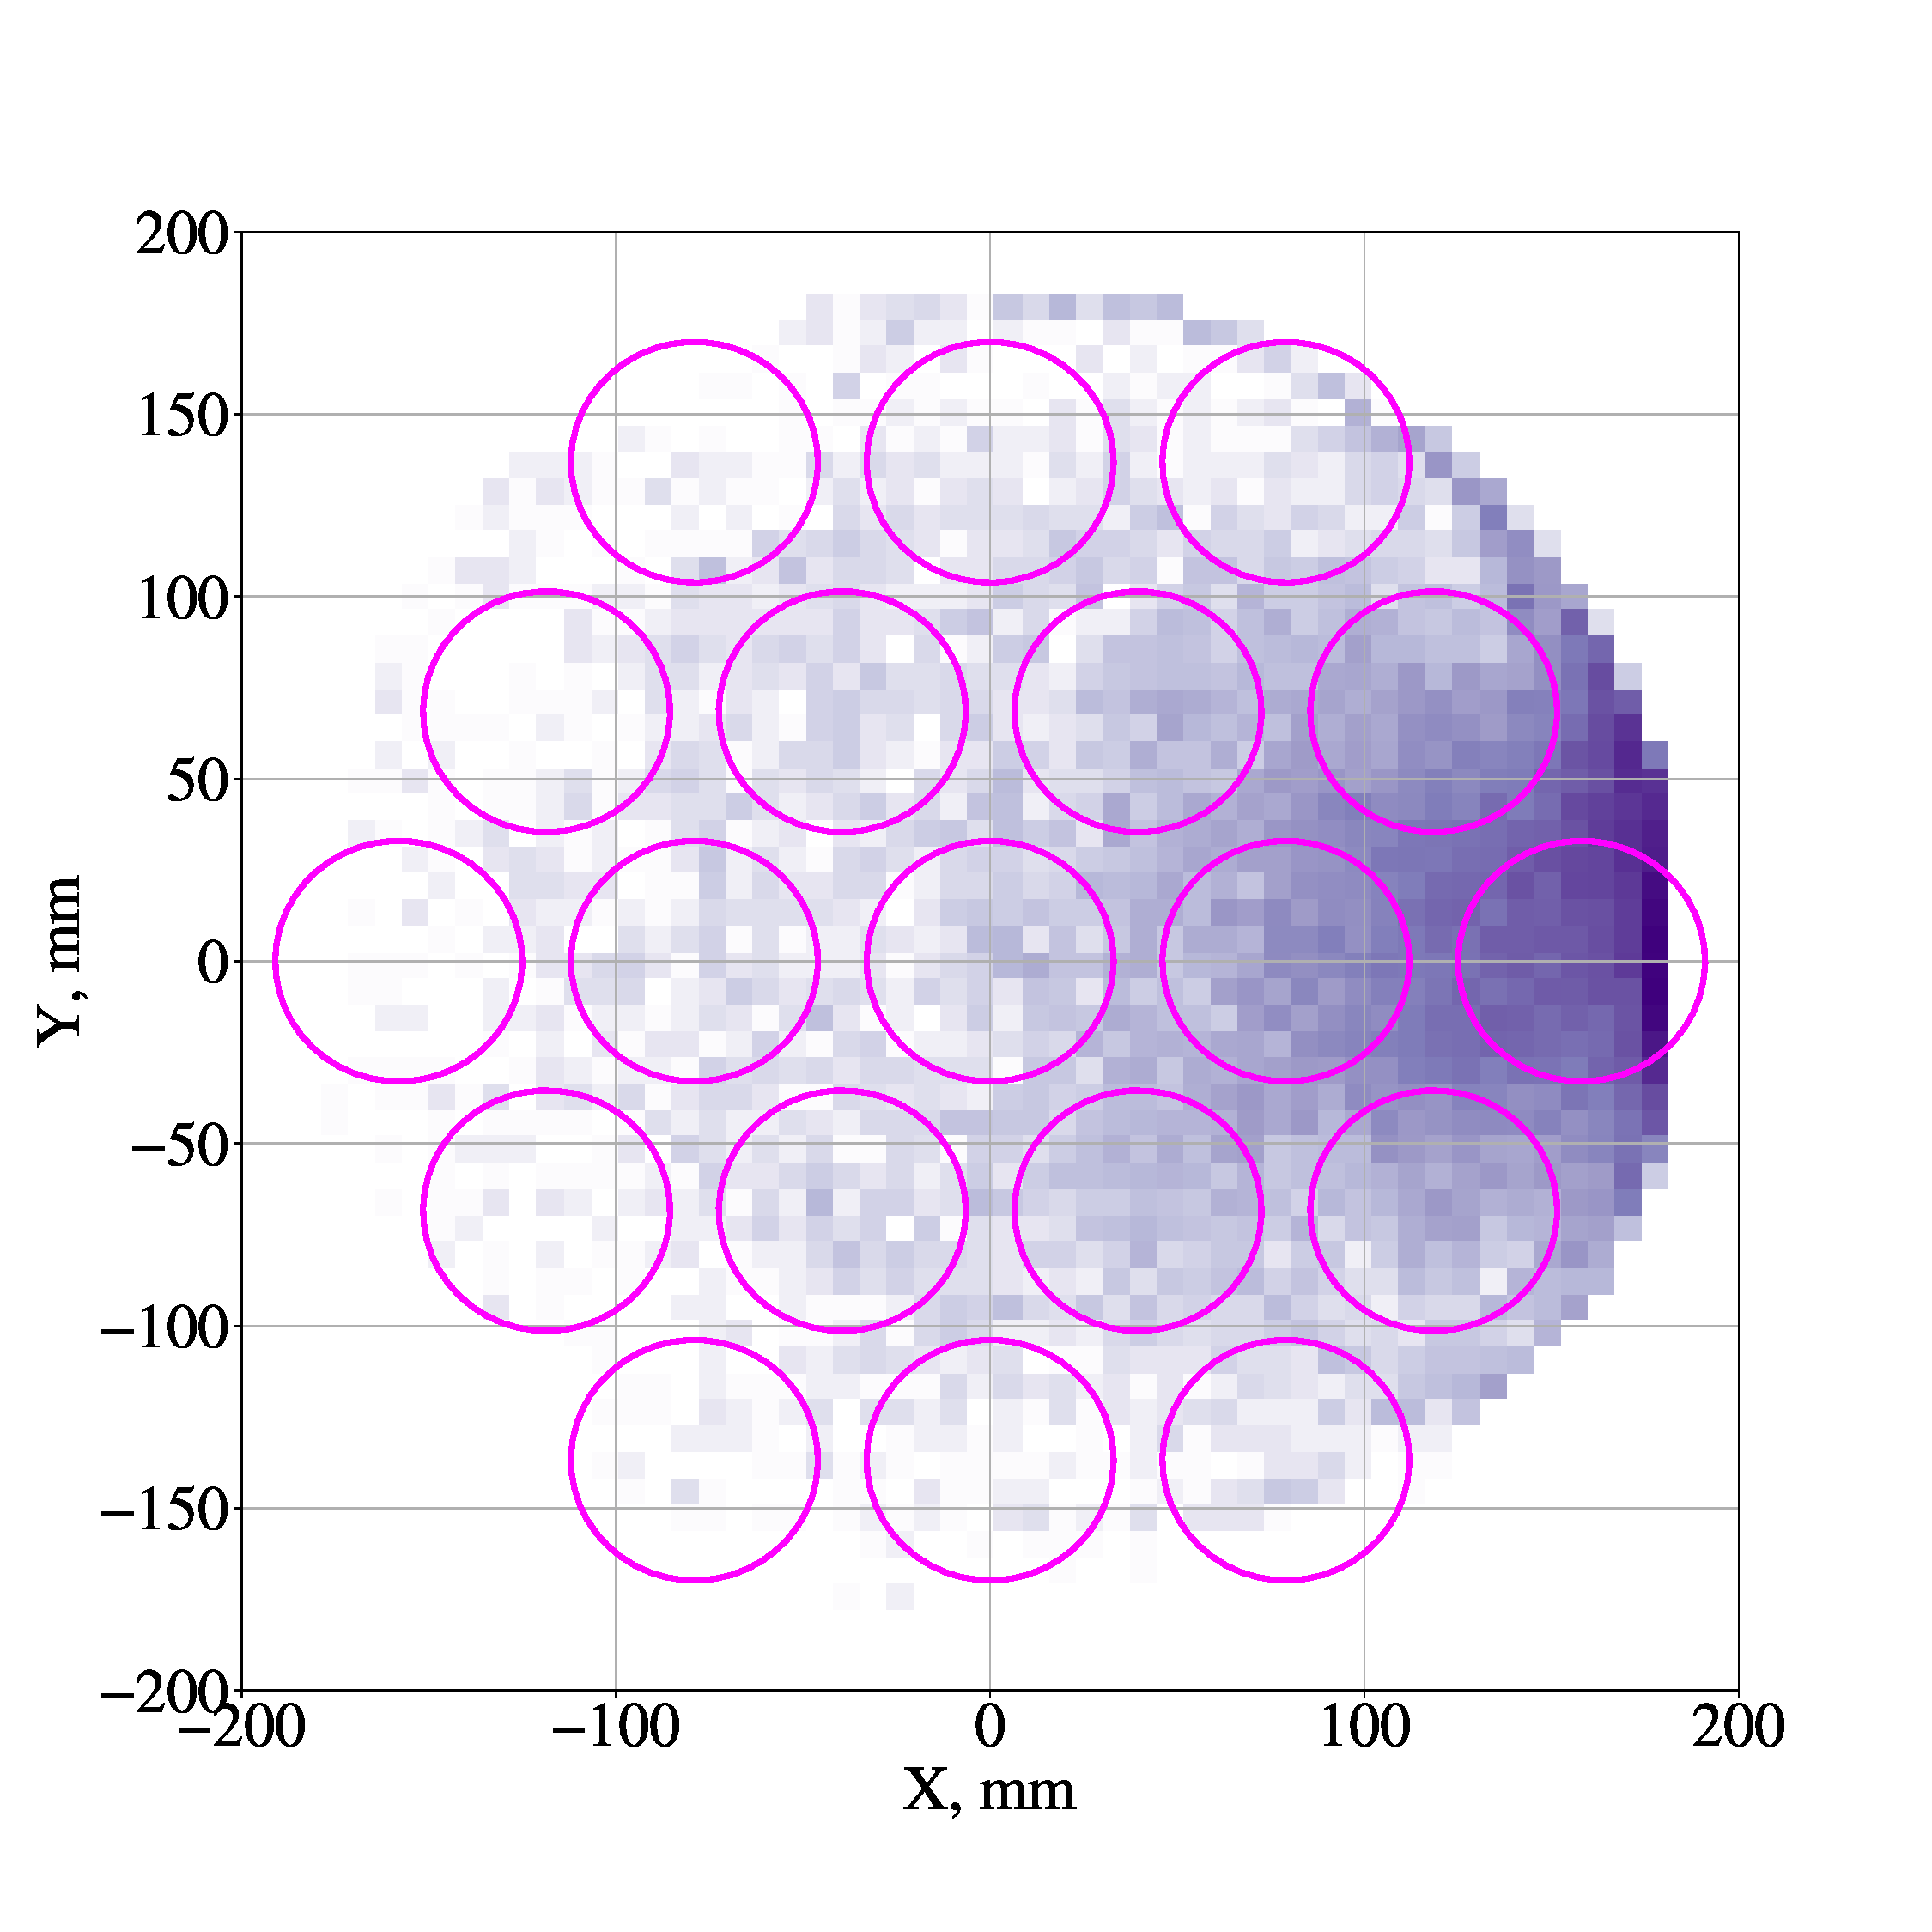
\includegraphics[width=0.6\linewidth]{images/NaXY.pdf}}
	\caption{Распределение по плоскости событий от $^{22}$Na во время инженерного сеанса}
	\label{img:xyplot2019}
\end{figure}

\begin{figure}[H]
	\center{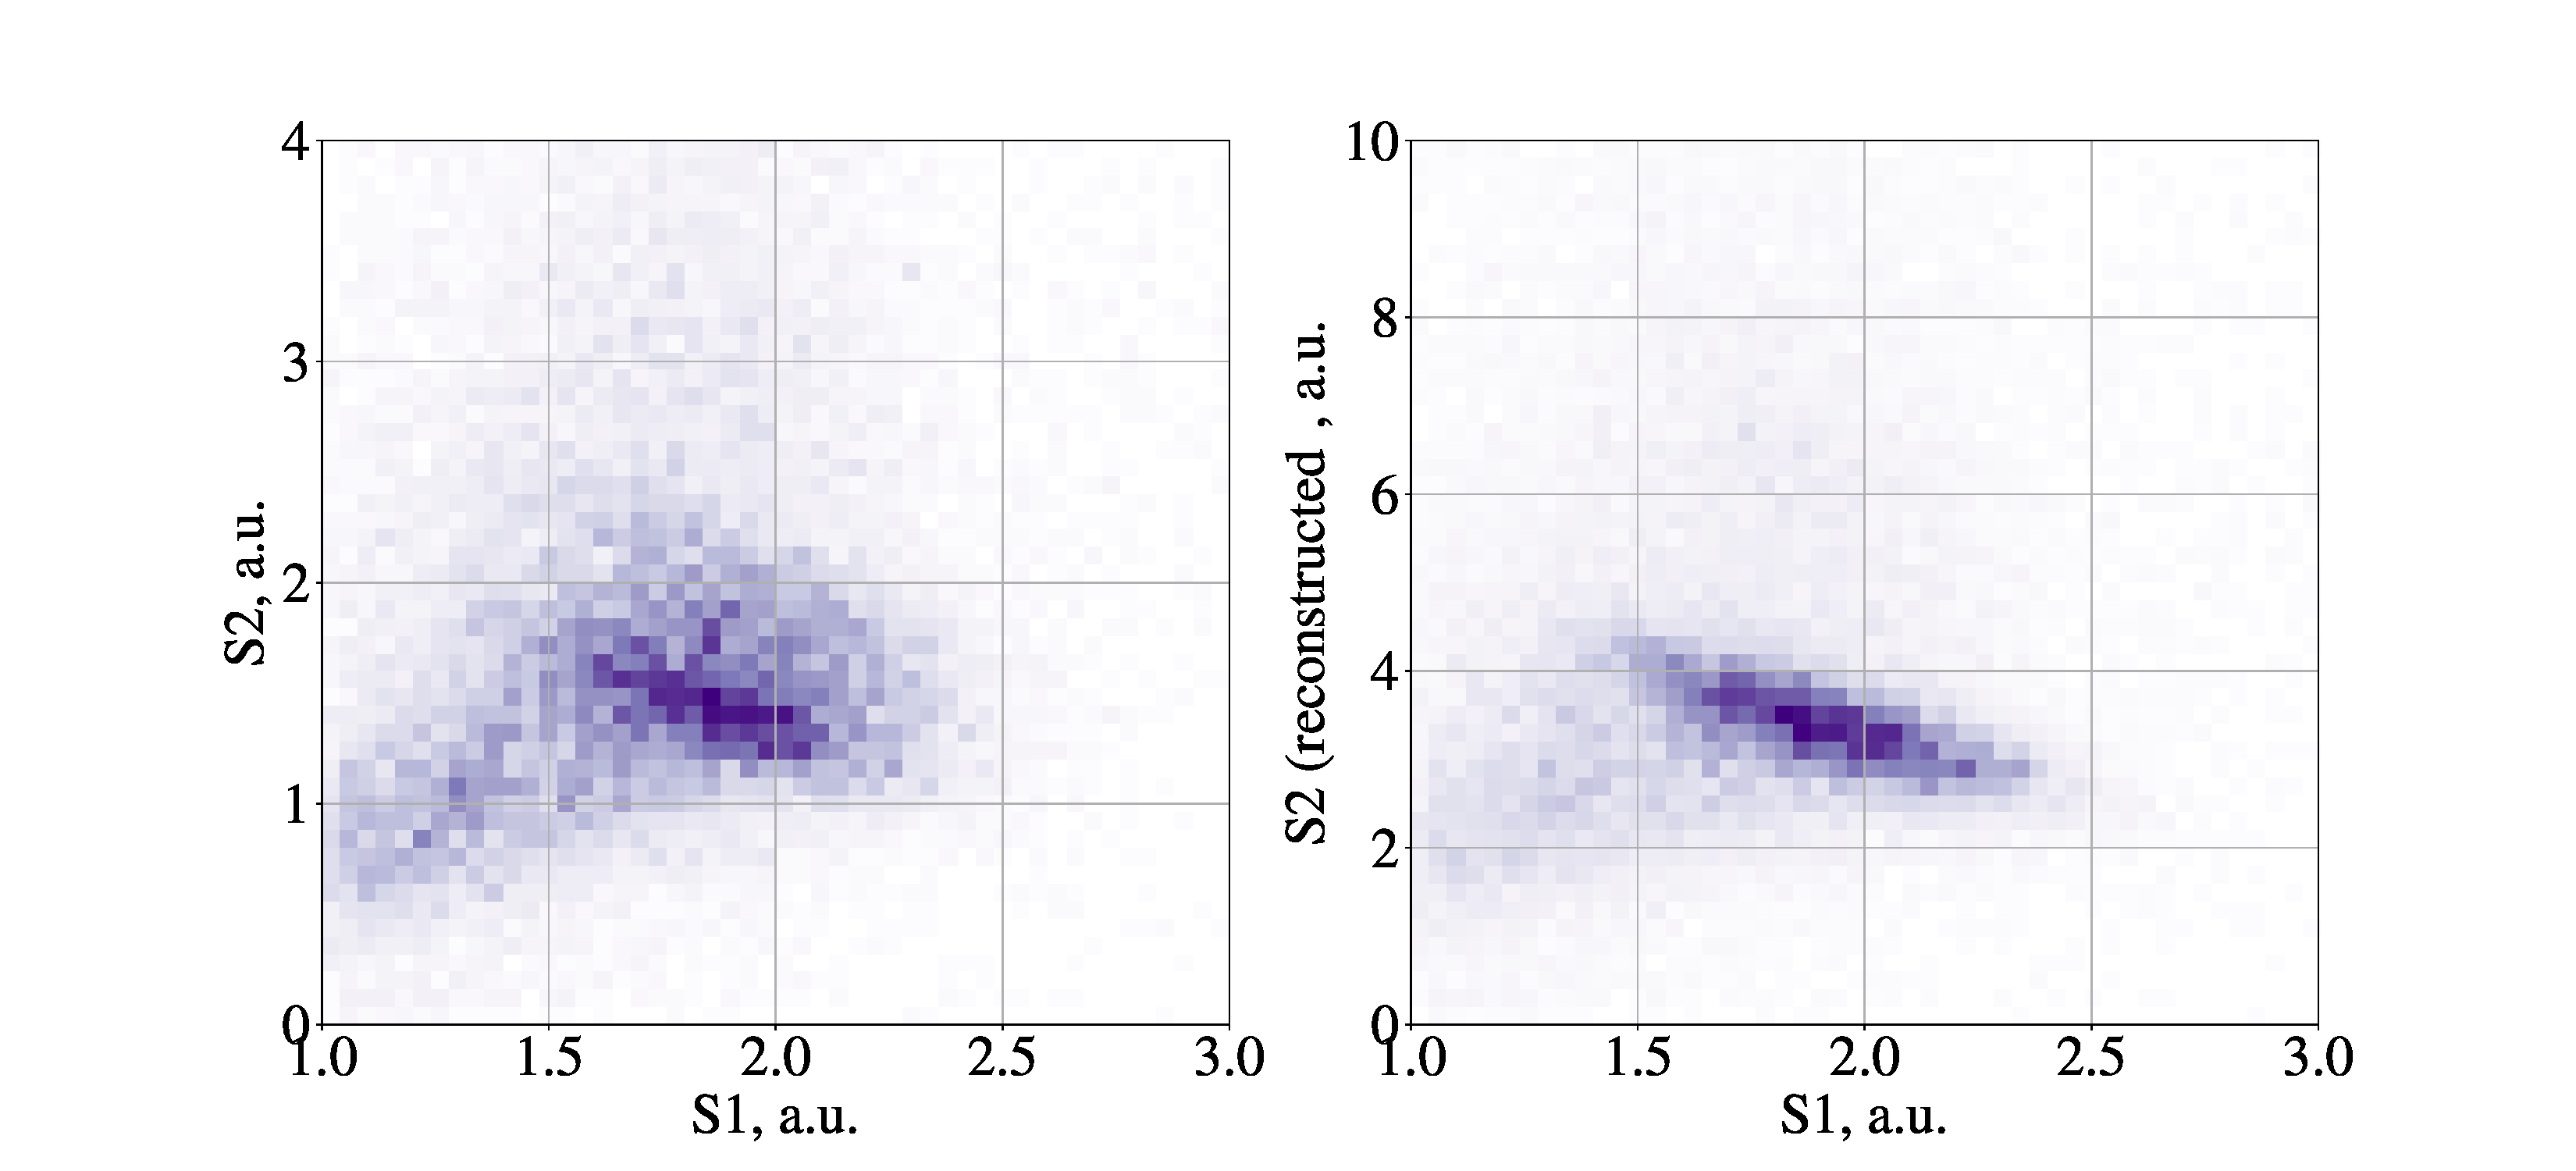
\includegraphics[width=1\linewidth]{images/Nas1s2.pdf}}
	\caption{Распределение событий по S1 и S2 для $^{22}$Na до(слева) и после(справа) восстановления}
  \label{img:s1s2na}  
\end{figure}

\begin{figure}[H]
	\center{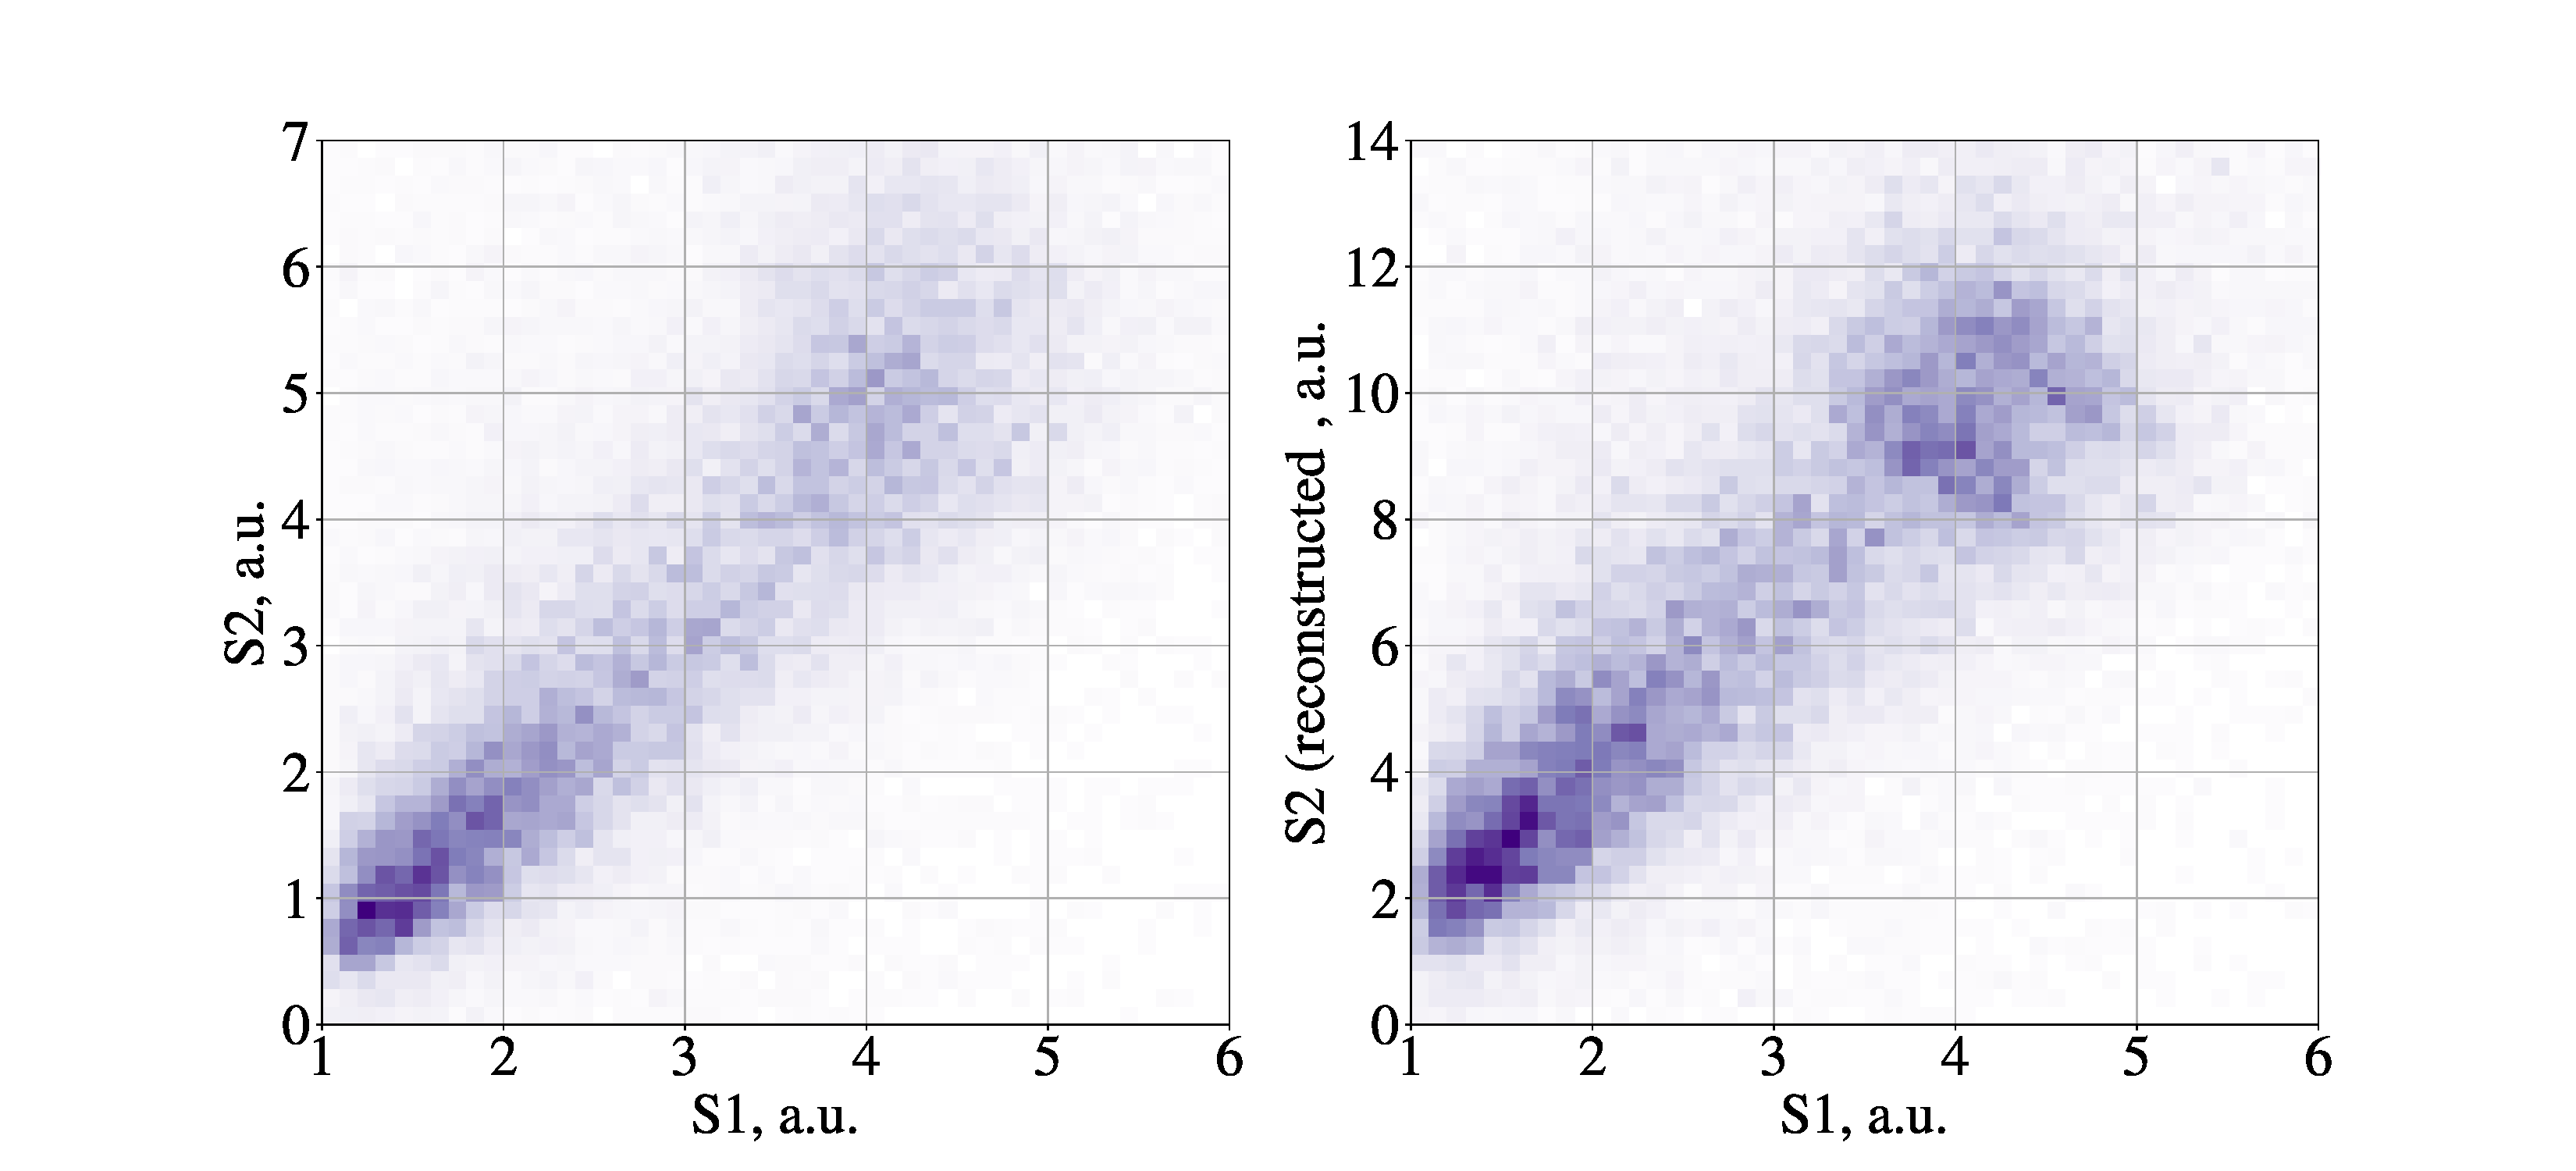
\includegraphics[width=1\linewidth]{images/Cos1s2.pdf}}
	\caption{Распределение событий по S1 и S2 для $^{60}$Co до(слева) и после(справа) восстановления}
  \label{img:s1s2co}  
\end{figure}

\begin{figure}[H]
\center{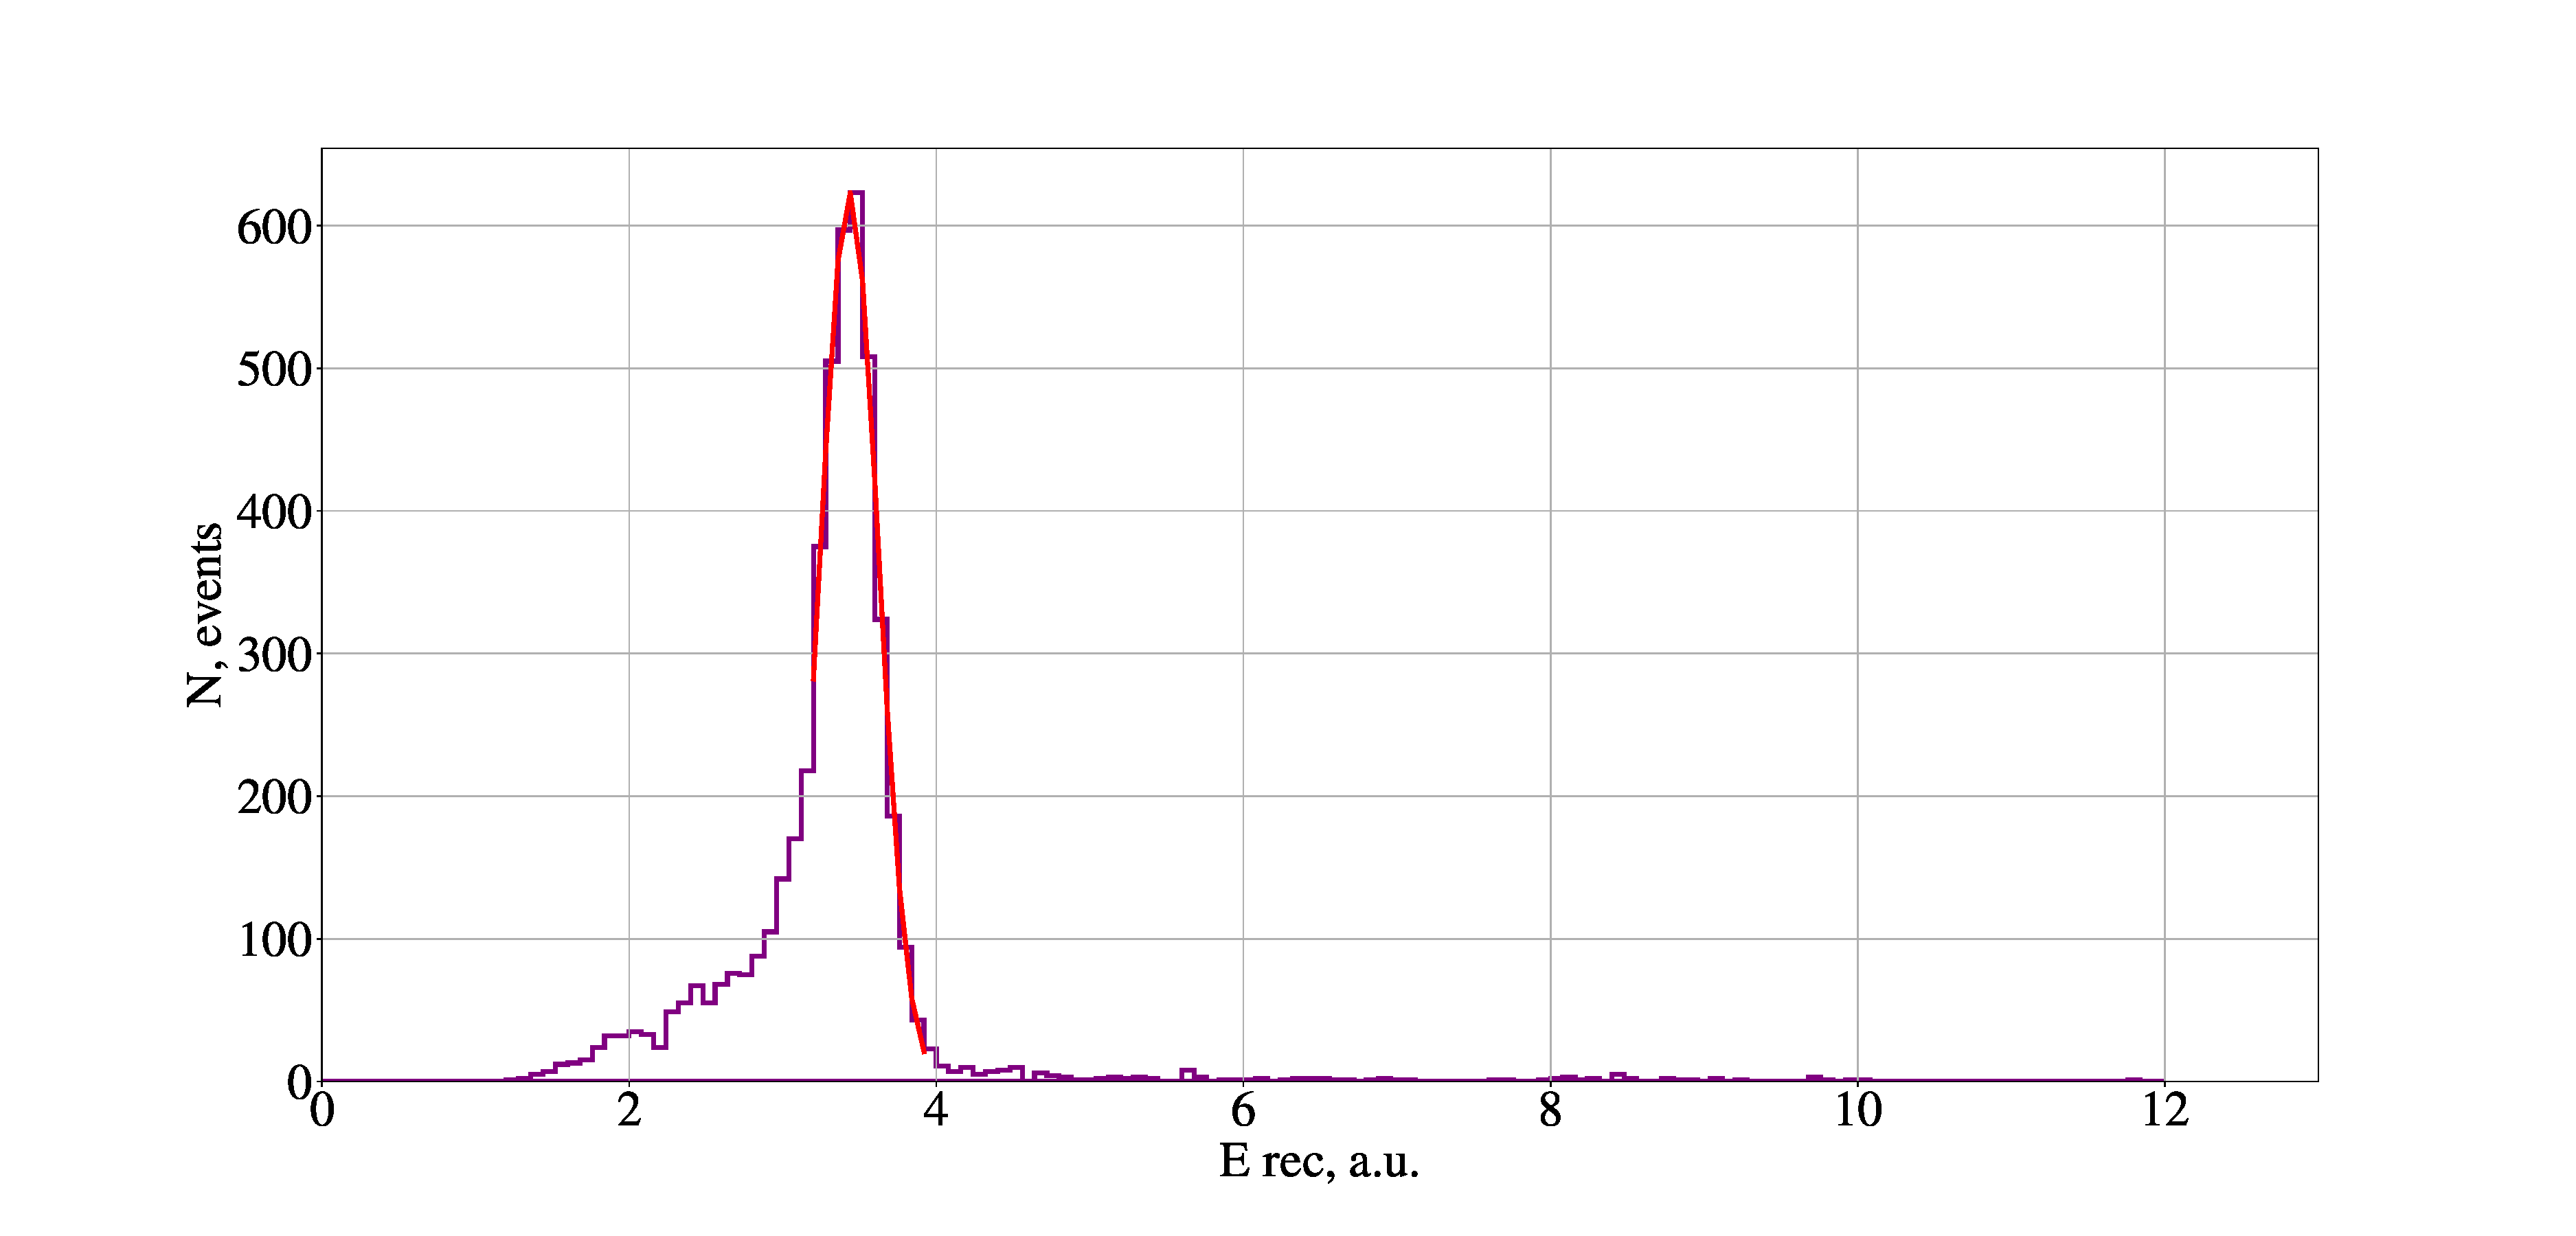
\includegraphics[width=1\linewidth]{images/linecomNa.pdf}}
  \caption{Энергетический спектр от источника $^{22}$Na после восстановления и его фитирование распределением Гаусса}
  \label{img:spectrNa}  
\end{figure}

\begin{figure}[H]
\center{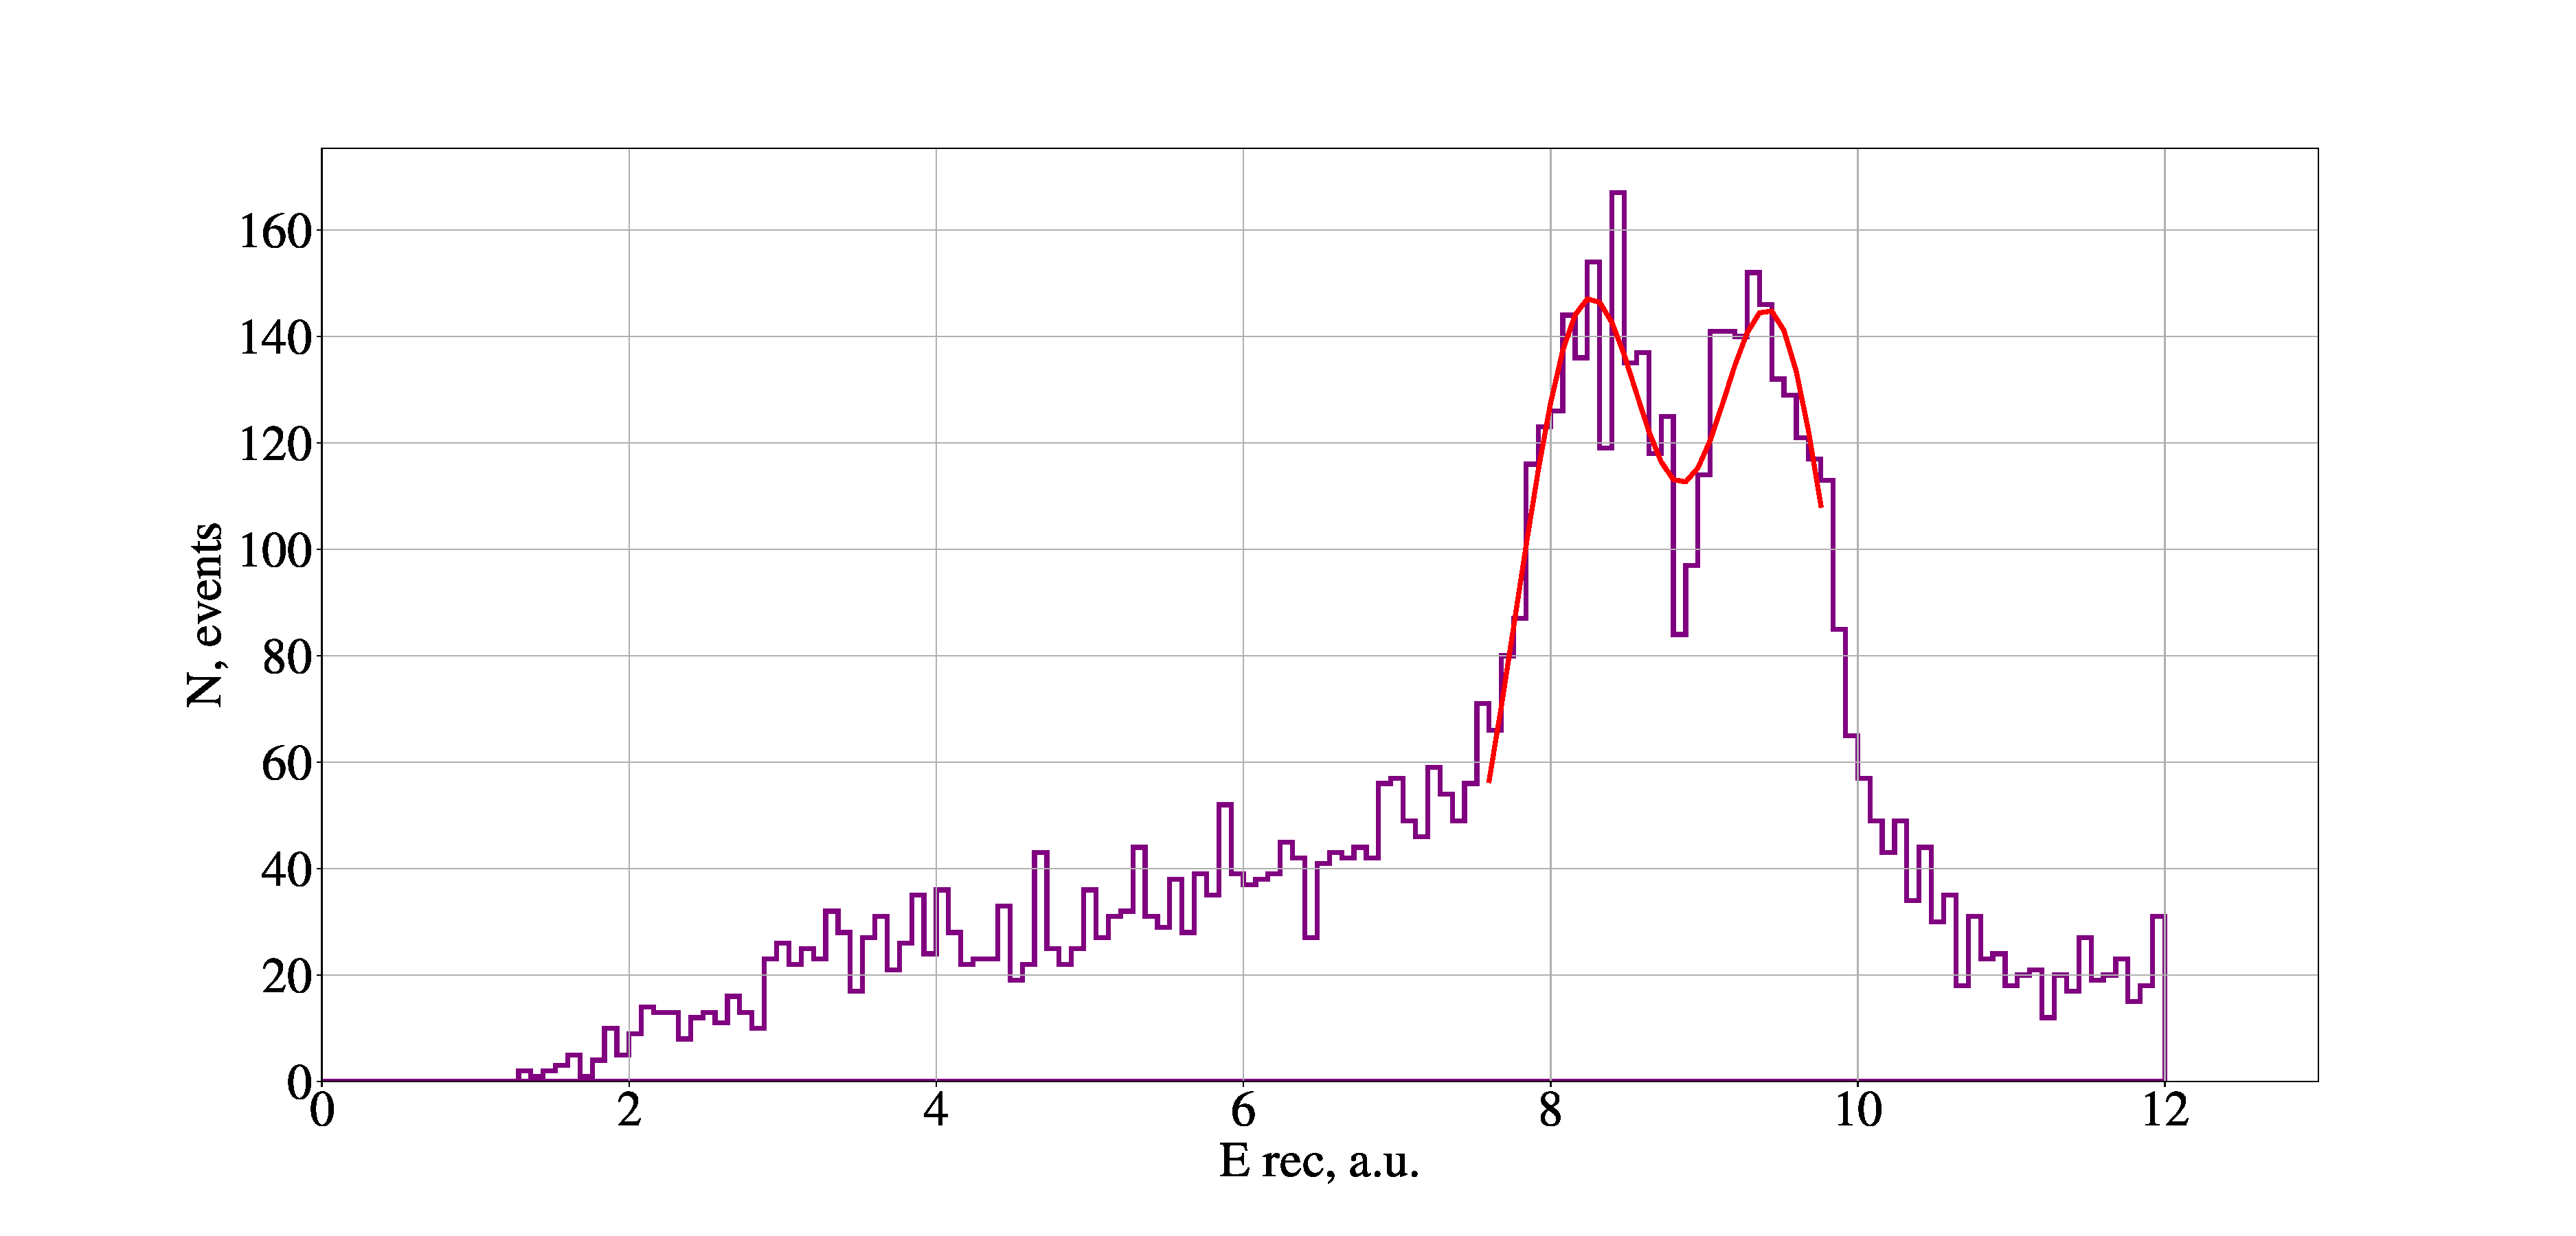
\includegraphics[width=1\linewidth]{images/linecomCo.pdf}}
  \caption{Энергетический спектр от источника $^{60}$Co после восстановления и его фитирование суммой двух распределений Гаусса}
  \label{img:spectrCo}  
\end{figure}

\begin{figure}[H]
\center{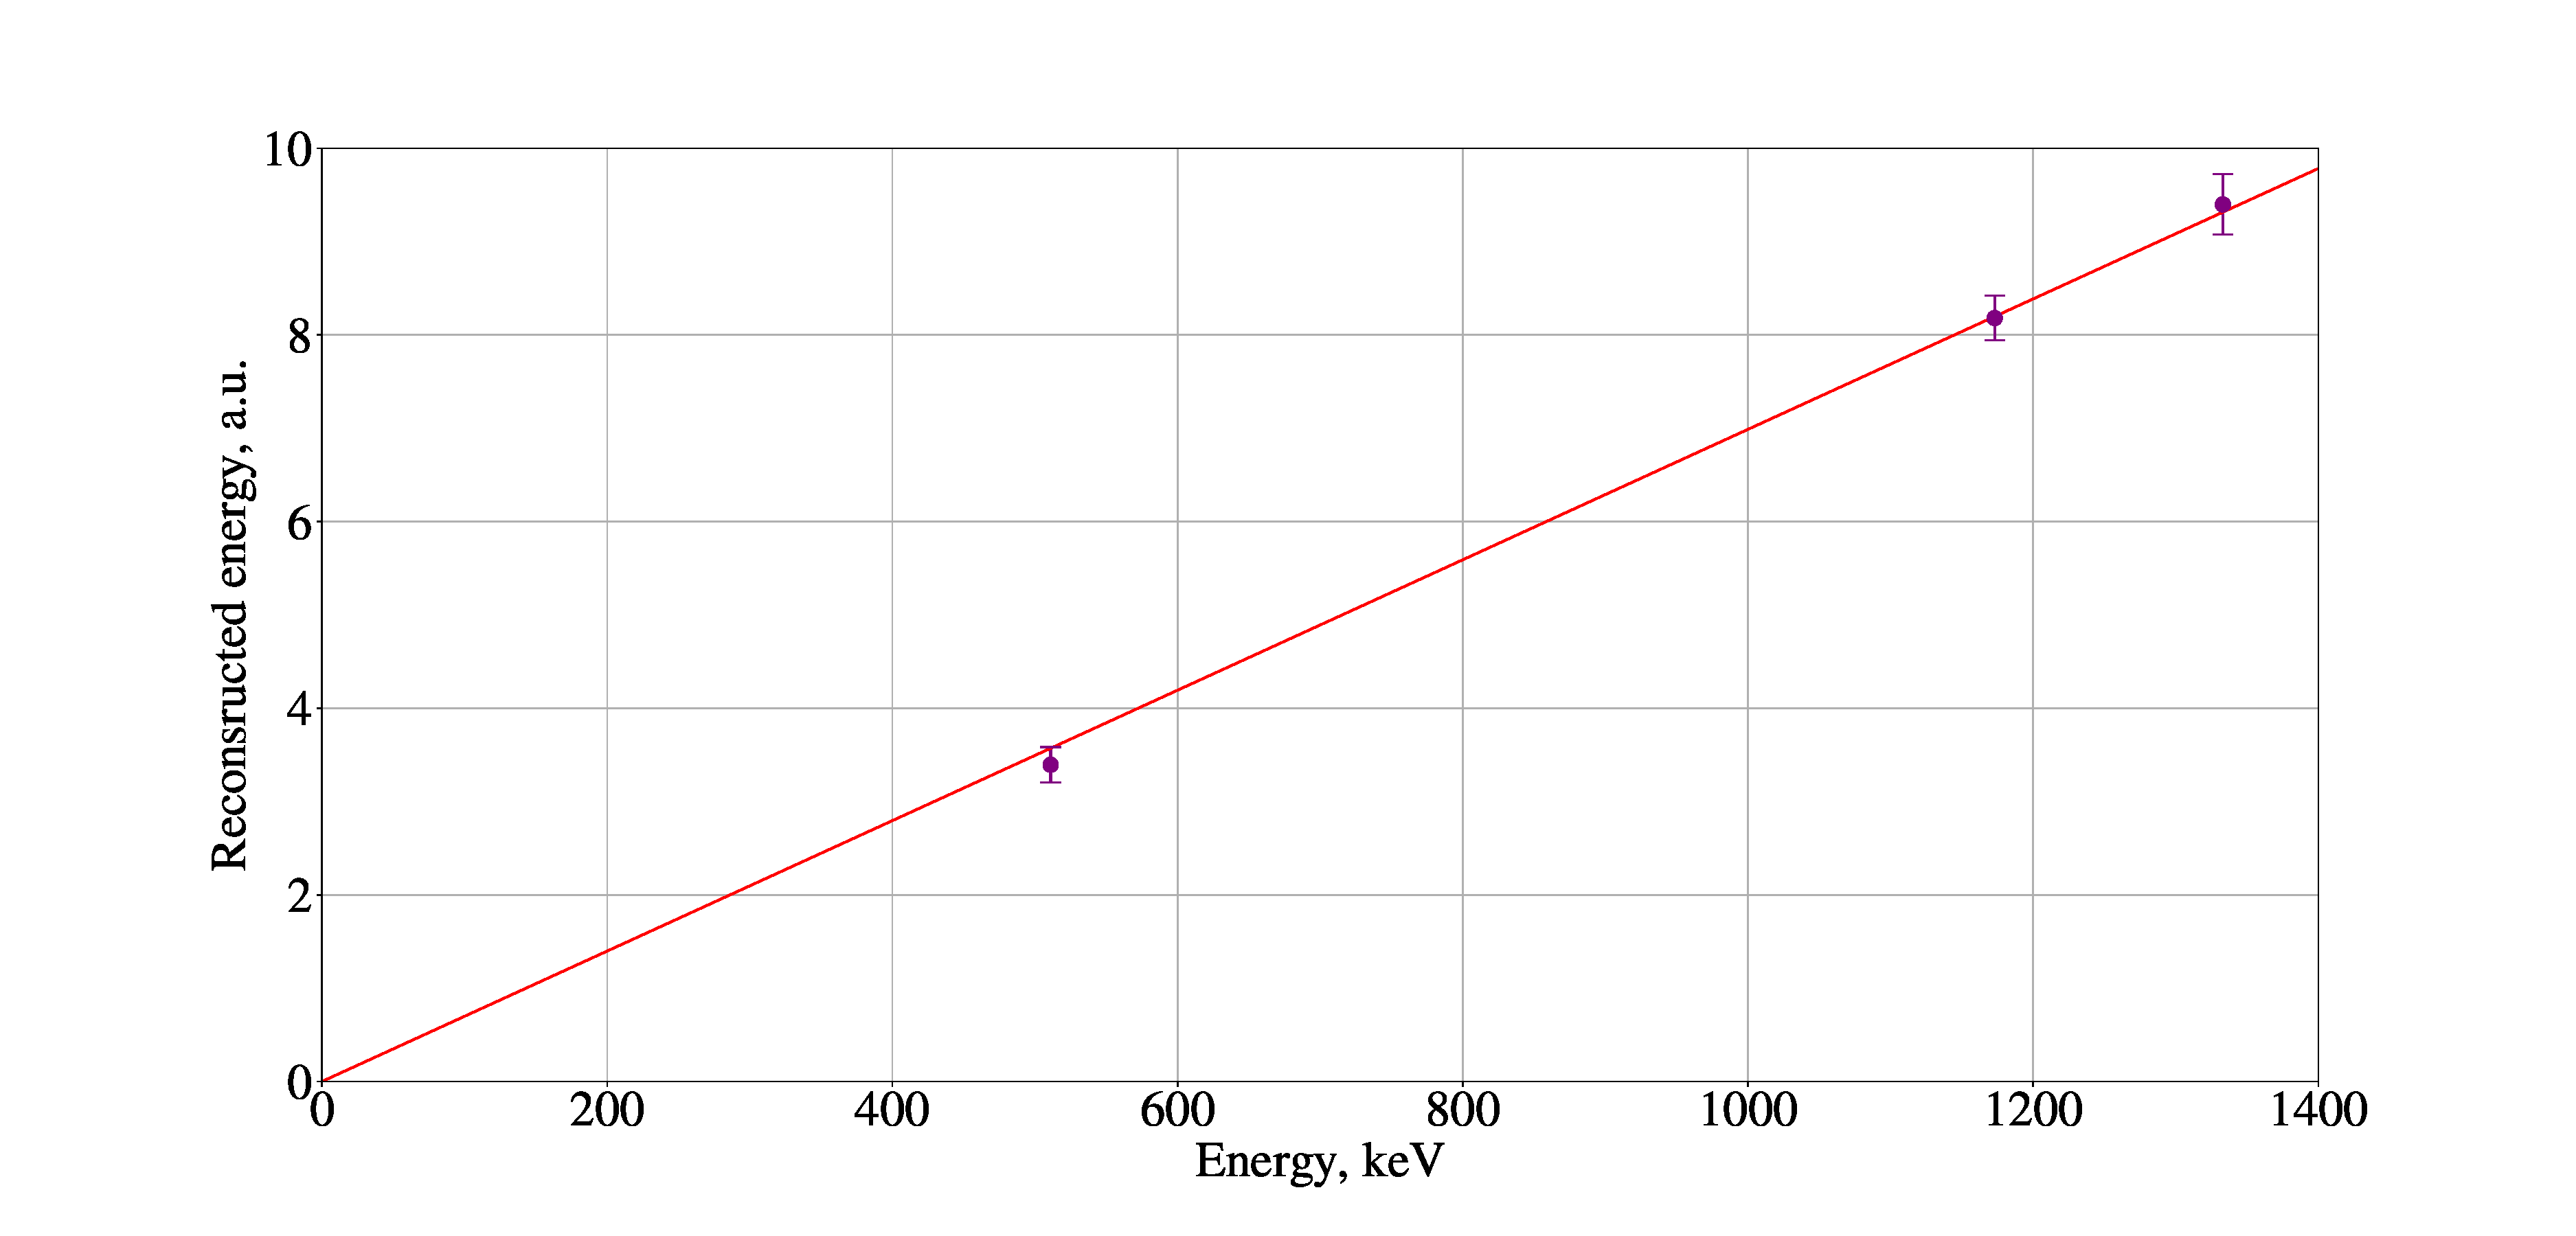
\includegraphics[width=1\linewidth]{images/calibr.pdf}}
  \caption{Калибровочный график для инженерного сеанса 2019 года.}
  \label{img:calibplot2019}  
\end{figure}

\begin{table}[hbt]
    \centering
        \caption{Положения пиков и энергетическое разрешение}
\begin{tabular}{|c|c|c|c|}
\hline
    Энергия, кэВ & Положение пика, кэВ & ($\sigma/E$), \% & FWHM/E,  \%\\
    \hline
    511 & 486$\pm$29 & 5.5$\pm$0.1 & 12.9$\pm$0.2\\
    \hline
    1173 & 1171$\pm$34 & 5.4$\pm$0.1 & 12.7$\pm$0.3\\
    \hline
    1333 & 1345$\pm$46 & 4.8$\pm$0.2 & 11.3$\pm$0.4\\
    \hline
\end{tabular}
    \label{tab:resolution2019}
\end{table}

\subsection{Калибровки гамма-источниками во время сеанса на Калининской АЭС}
\label{subsect3_3_5}

 
\parК сожалению, измерения с гамма-источниками при постановке эксперимента на КАЭС заведомо имели меньшую точность, чем измерения во время инженерного сеанса. Это связано с невозможность коллимирования источников, набора достаточно хорошей статистики и использования схемы совпадений. Кроме того, конструкция установки с учетом пассивной защиты не позволяла расположить источники достаточно близко к криостату детектора.
\parАлгоритмы анализа данных принципиально не отличались, однако были скорректированы параметры отборов. Так, для улучшения соотношения сигнал/фон, отбирались события, находящиеся внутри радиуса 130 мм, аналогичный отбор по радусу в дальнейшем применялся для всех остальных данных, для которых производилось восстановление.
\parНа рисунке~\ref{img:s1s2Co2022} представлены двумерные распределения S1 и S2 до и после восстановления. На рисунке~\ref{img:spectrCo2022} представлен энергетический спектр от источника $^{60}$Co после восстановления и его фитирование суммой двух распределений Гаусса и функции ошибок, описывающей фон. В таблице~\ref{tab:resolution2022} представлены результаты калибровки гамма-источниками, а на рисунке~\ref{img:calibr2022} -- калибровочный график. Видно, что несмотря на худшую статистику энергетическое разрешение для кобальта улучшилось по сравнению с инженерным сеансом. Это связано с существенно более жестким отбором по радиусу (130 мм вместо 175 мм во время инженерного сеанса), а также введением дополнительно функции ошибок для описания фона.
\begin{figure}[H]
\center{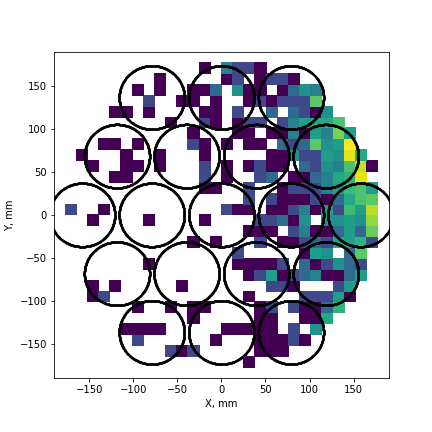
\includegraphics[width=0.5\linewidth]{images/xy_distr.png}}
  \caption{Распределение по плоскости событий от источника $^{60}$Co во время сеанса на КАЭС}
  \label{img:xyCo2022}  
\end{figure}

\begin{figure}[ht]
  \begin{minipage}[ht]{0.49\linewidth}    \center{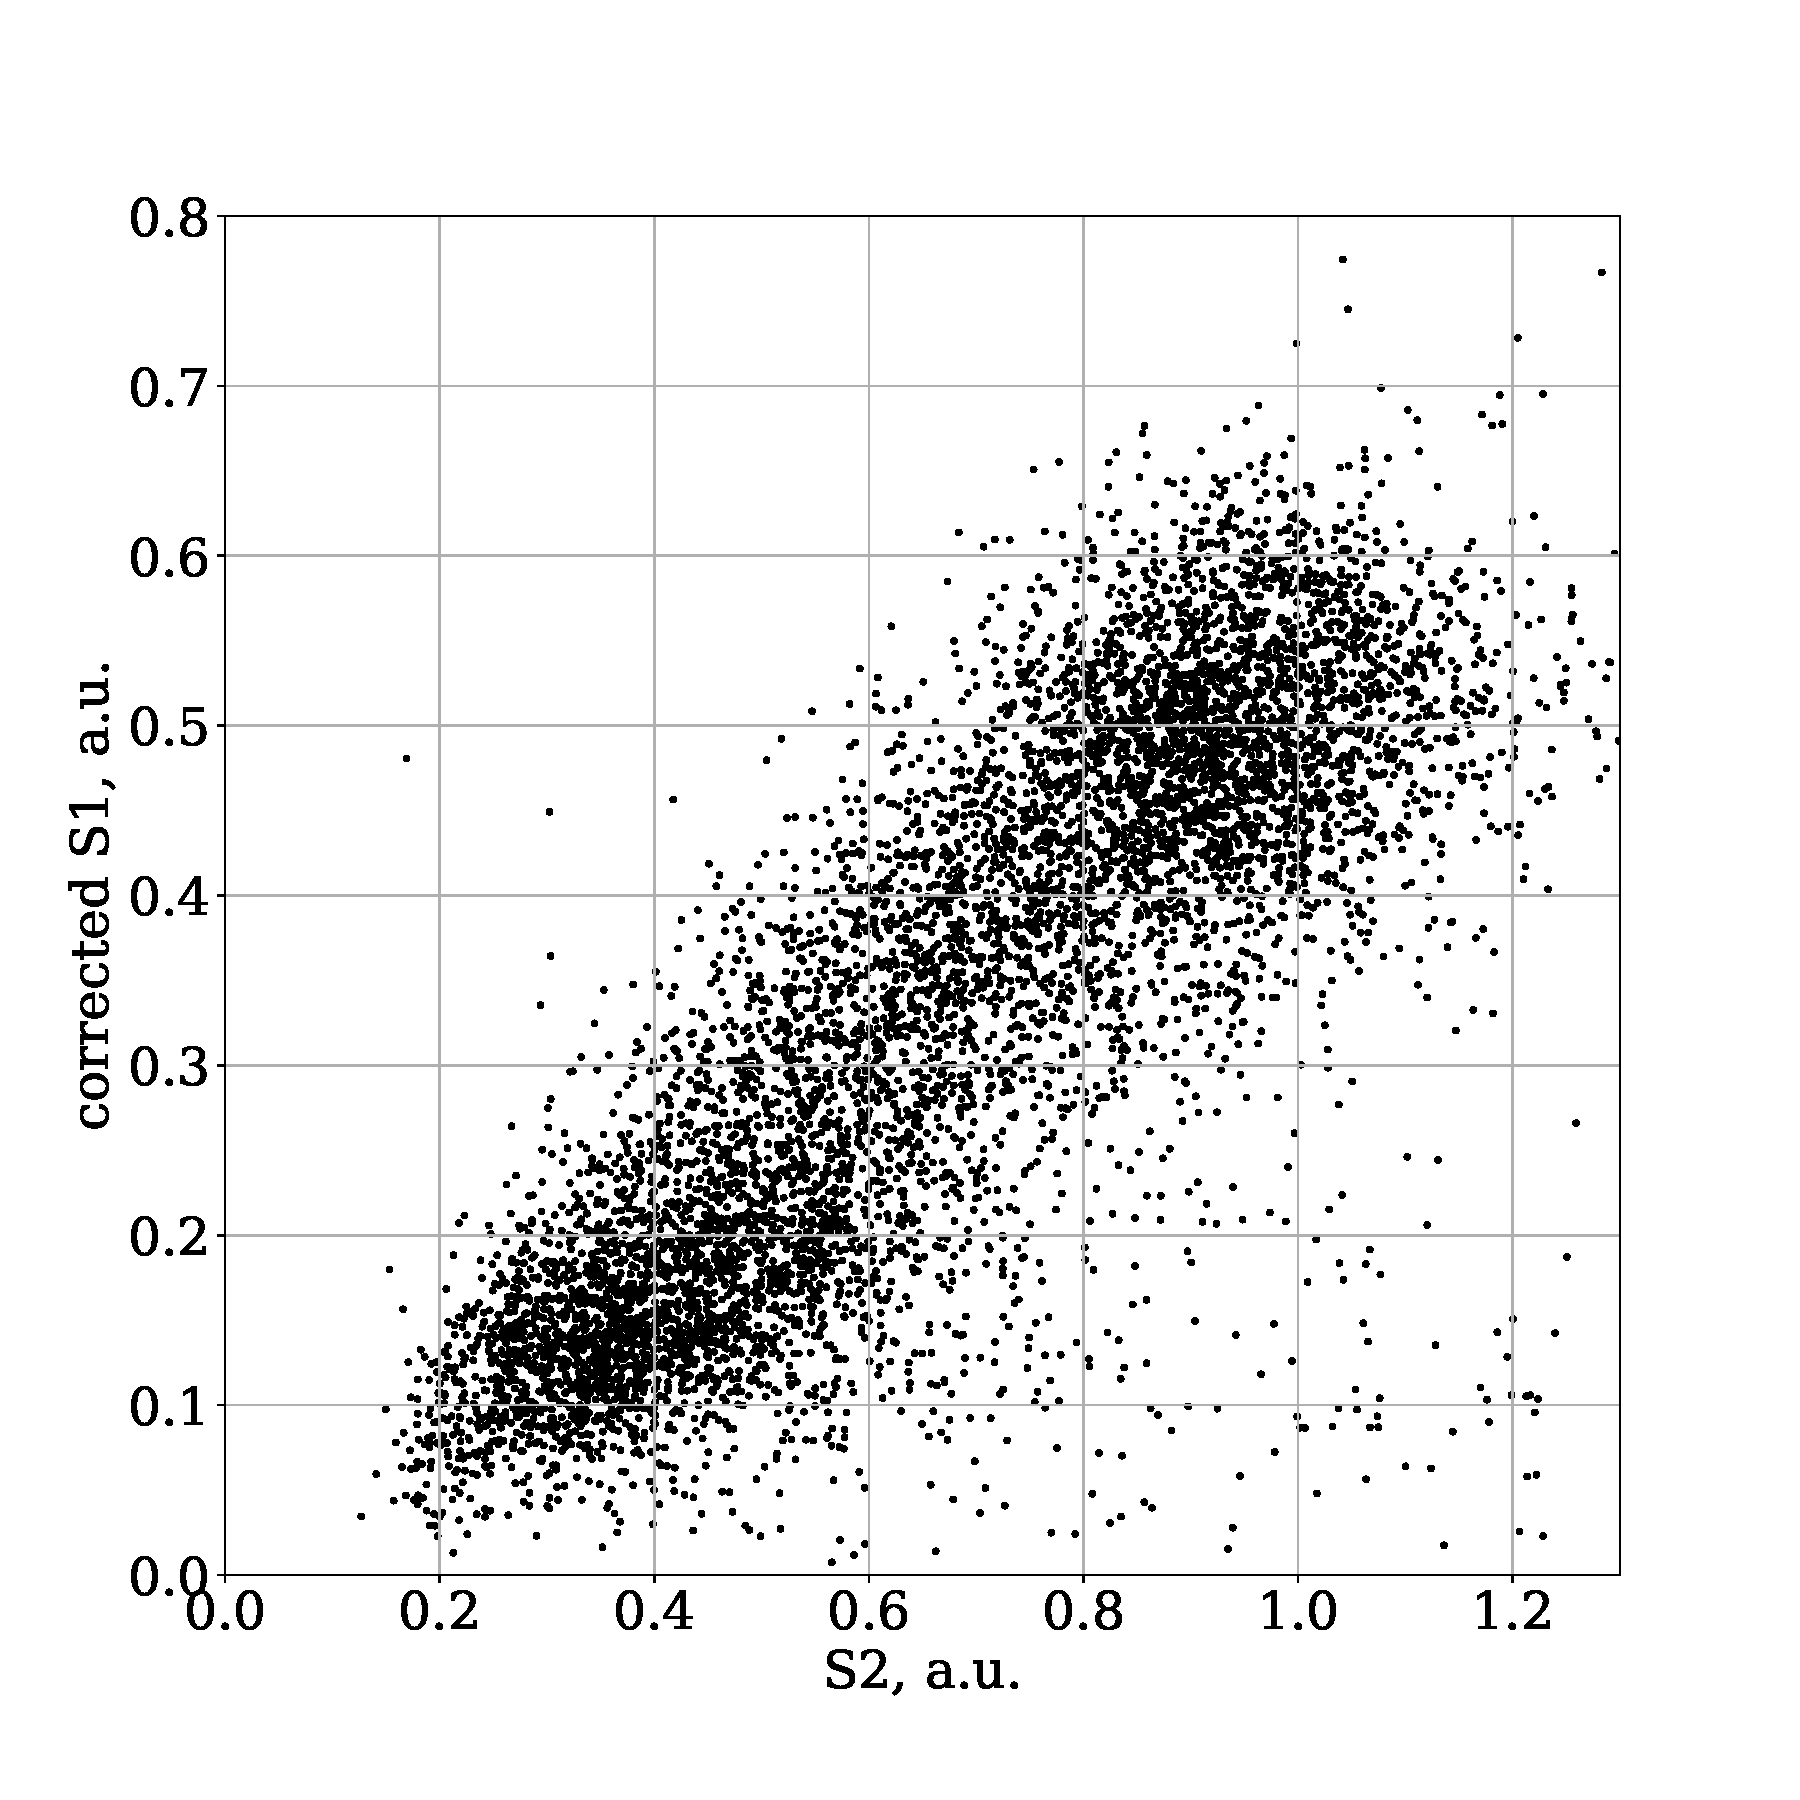
\includegraphics[width=1.0\linewidth]{images/2dspectrum.pdf} \\ а)}
  \end{minipage}
  \hfill
  \begin{minipage}[ht]{0.49\linewidth}  \center{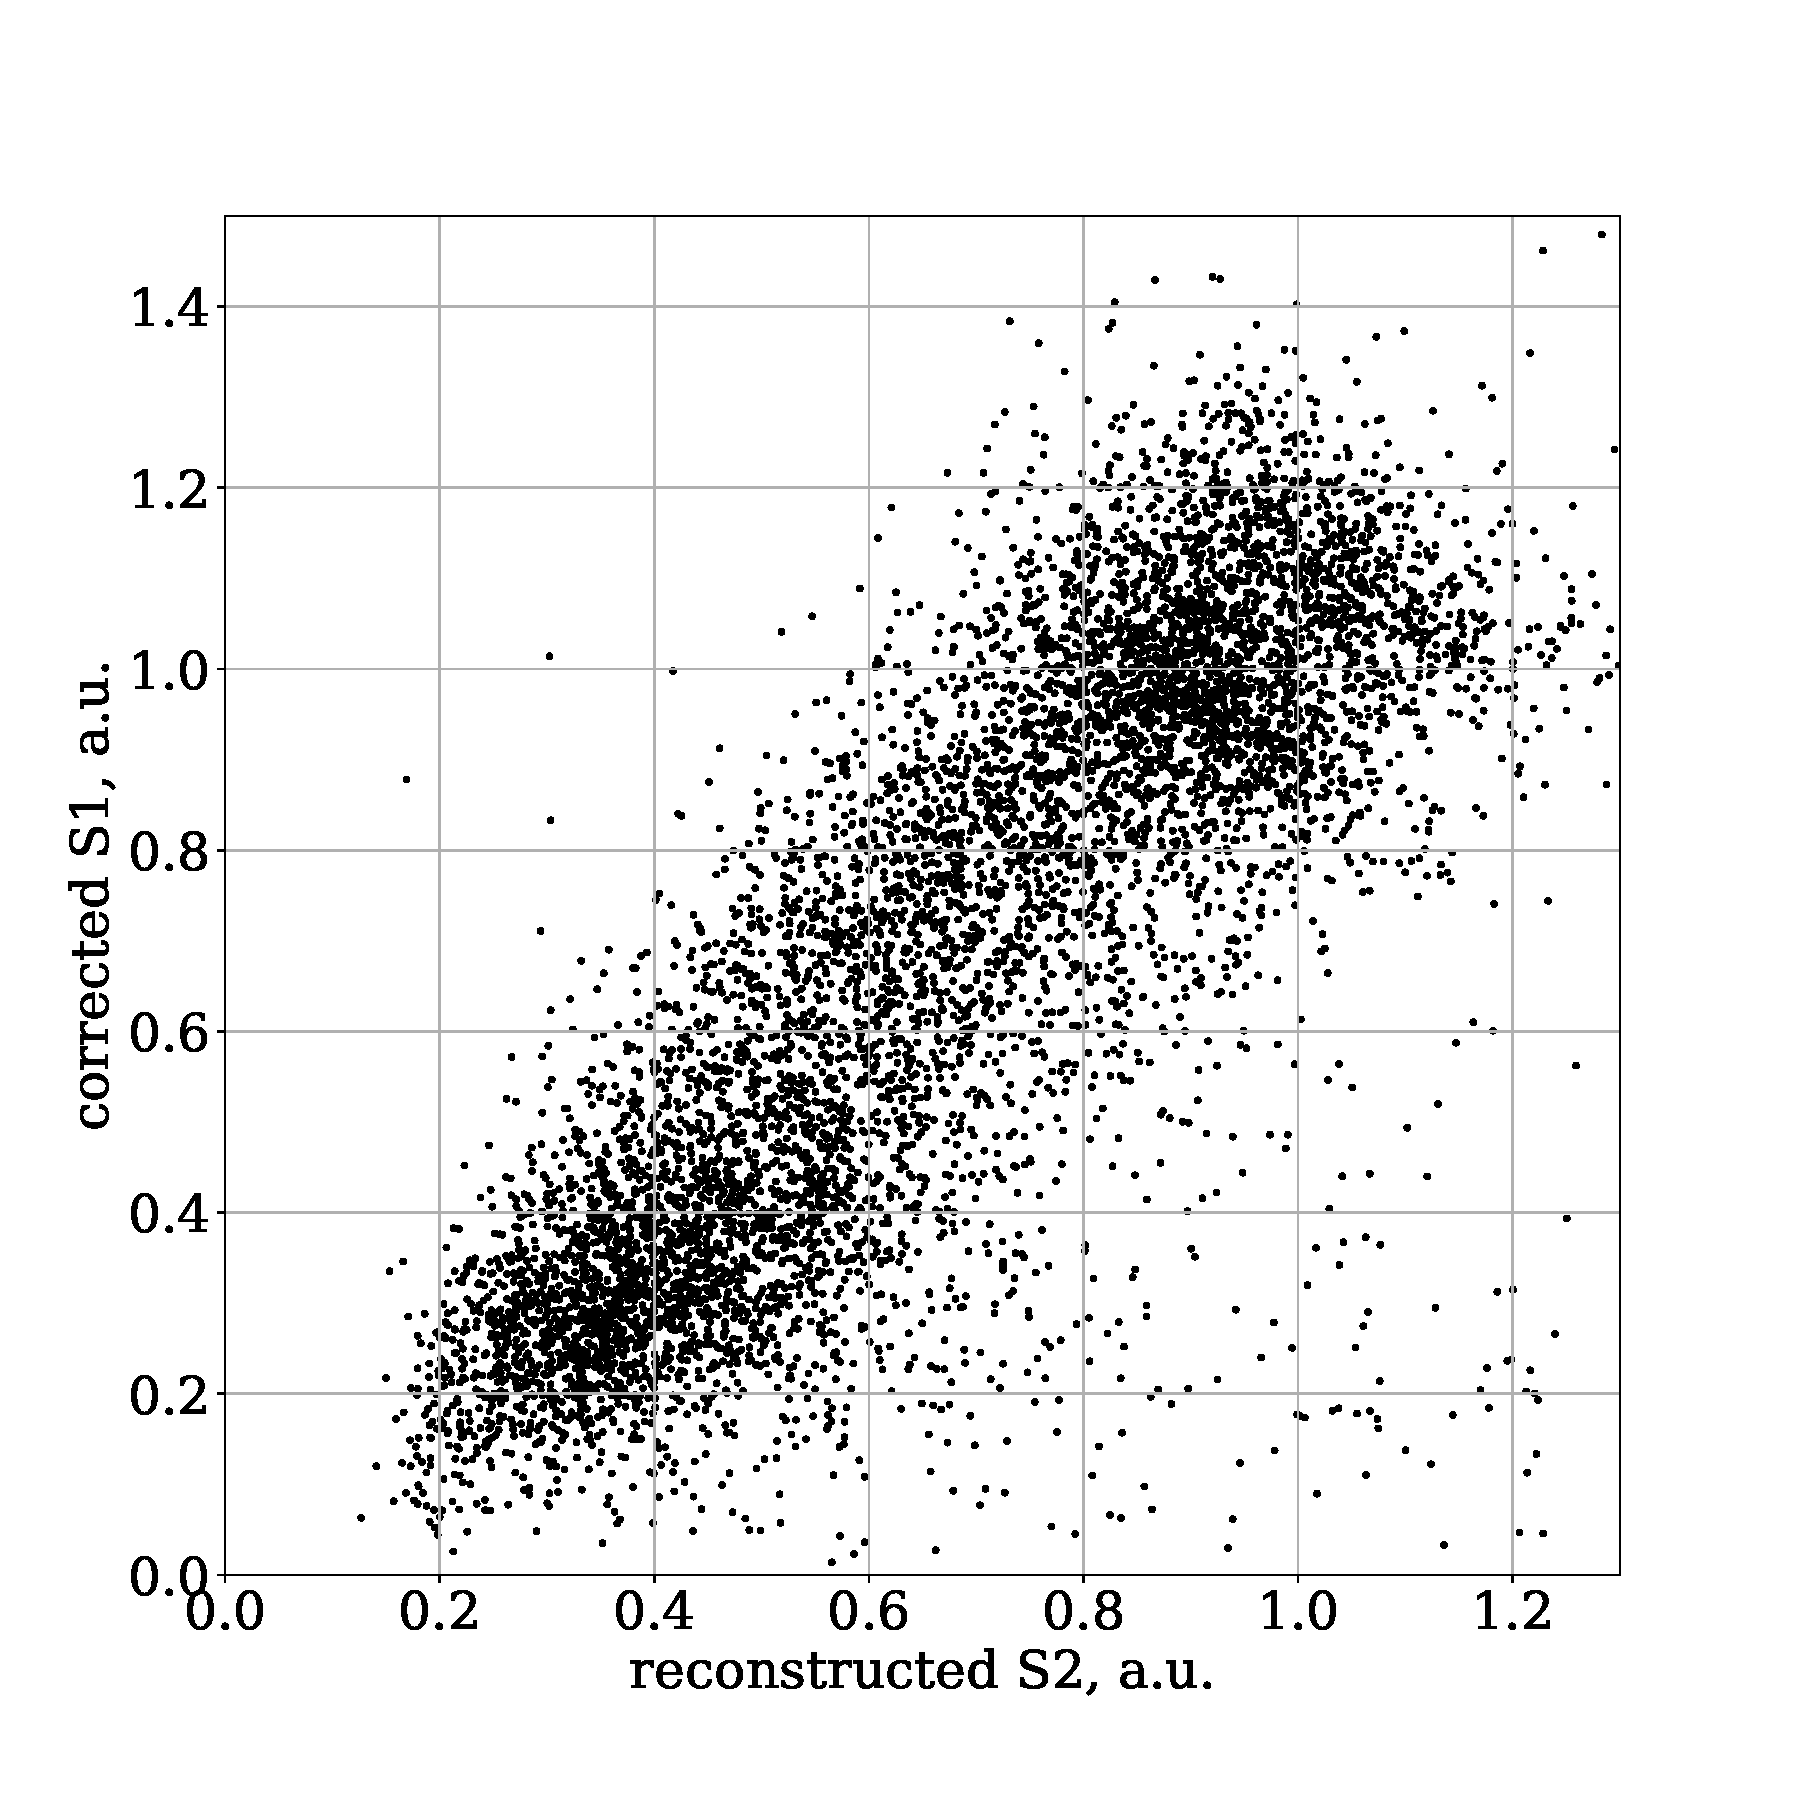
\includegraphics[width=1.0\linewidth]{images/2dspectrum_corr.pdf} \\ б)}
  \end{minipage}
  \caption{Распределение событий по S1 и S2 для $^{60}$Co до(слева) и после(справа) восстановления (сеанс на КАЭС)}
  \label{img:s1s2Co2022}  
\end{figure}

\begin{figure}[H]
\center{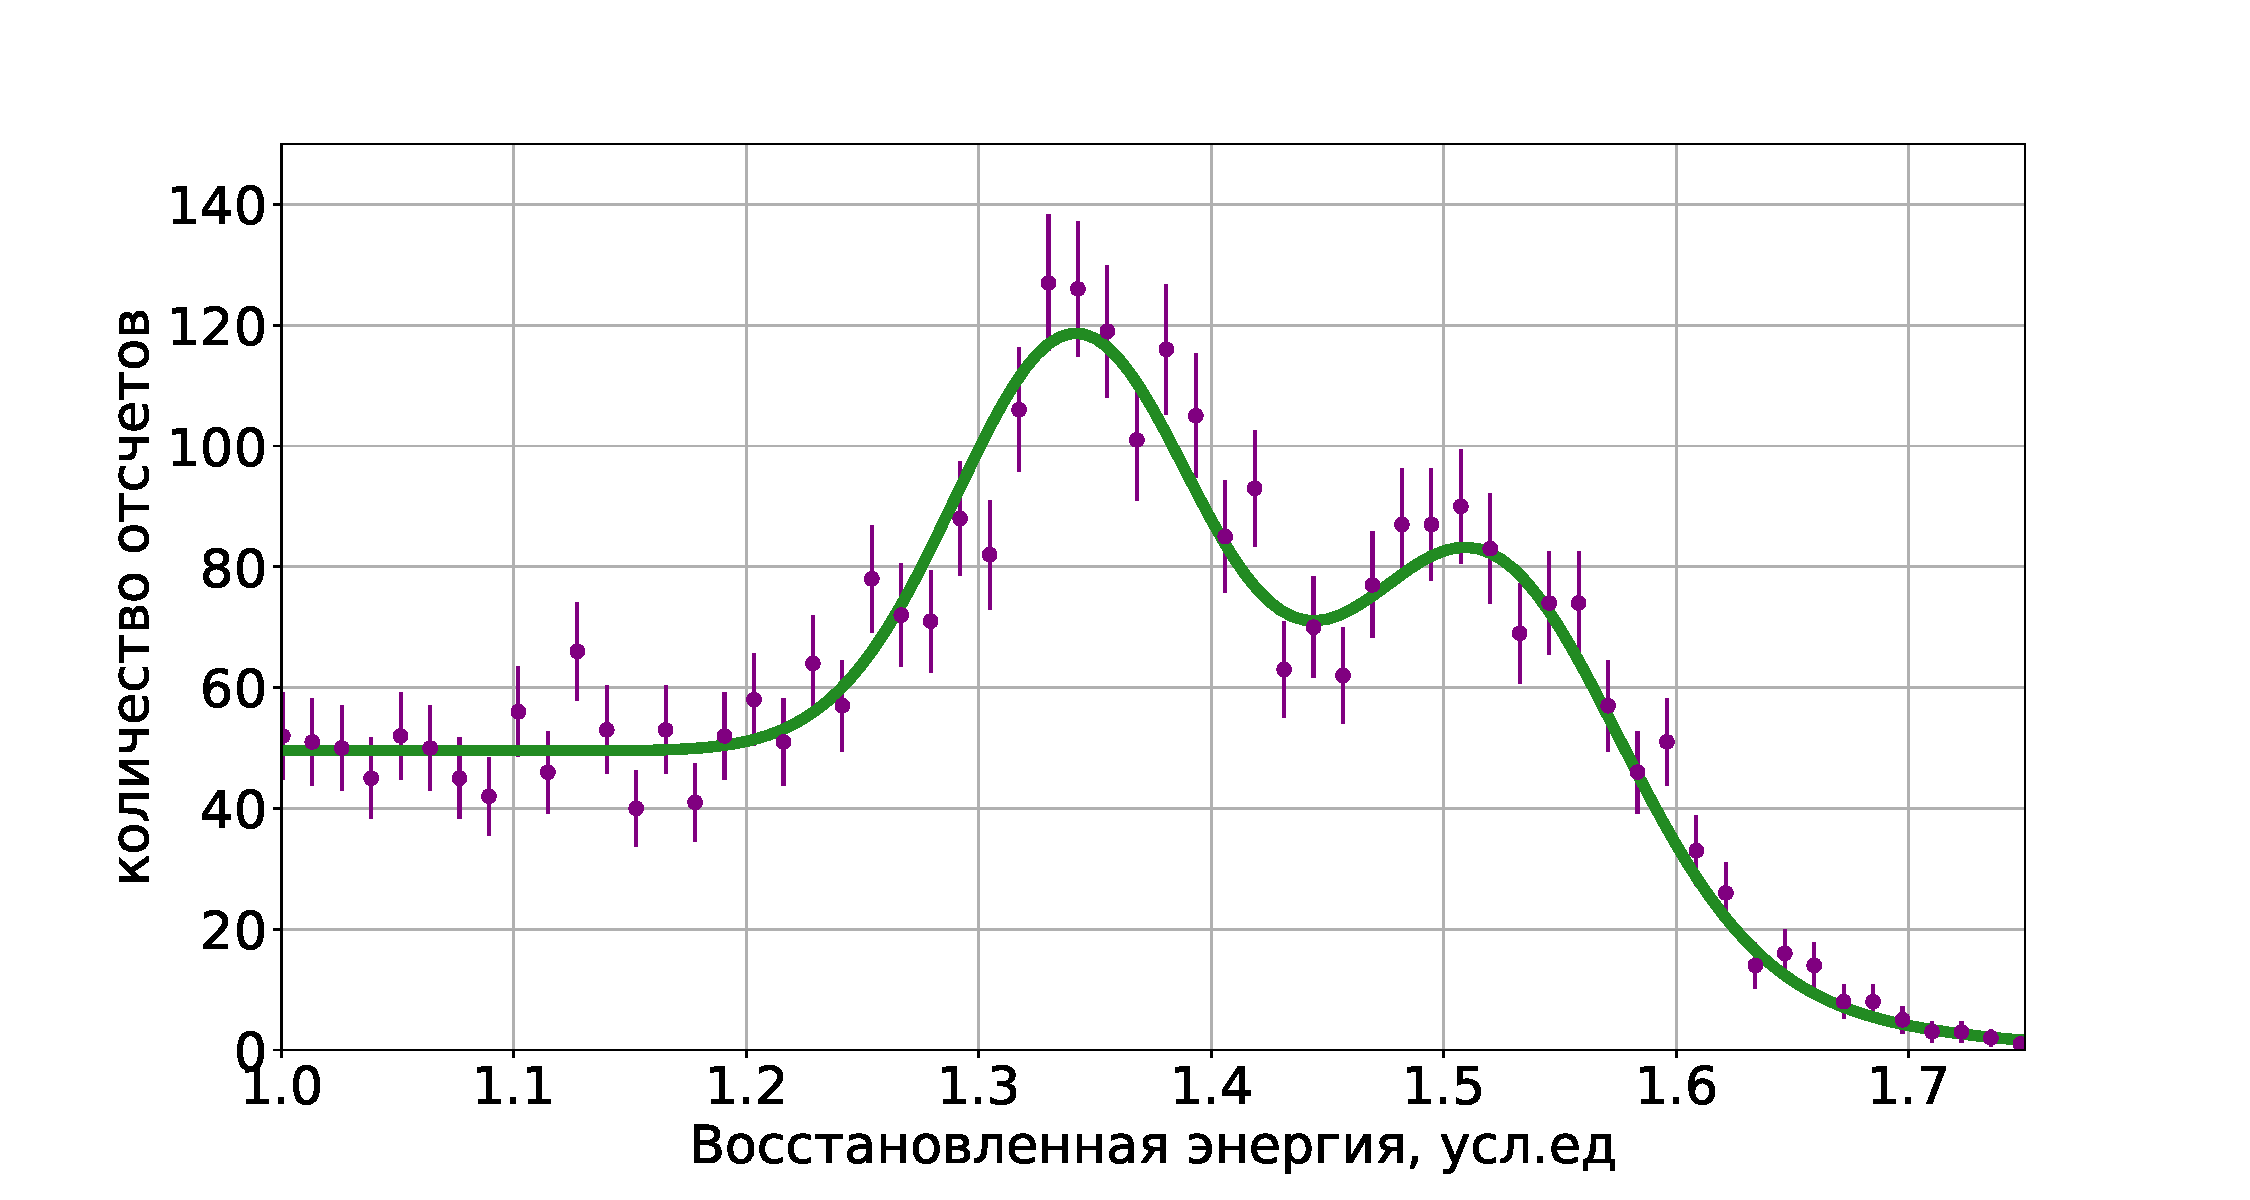
\includegraphics[width=1\linewidth]{images/spectrco2022.pdf}}
  \caption{Энергетический спектр от источника $^{60}$Co после восстановления и его фитирование суммой двух распределений Гаусса и функции ошибок, описывающей фон}
  \label{img:spectrCo2022}  
\end{figure}

\begin{figure}[H]
\center{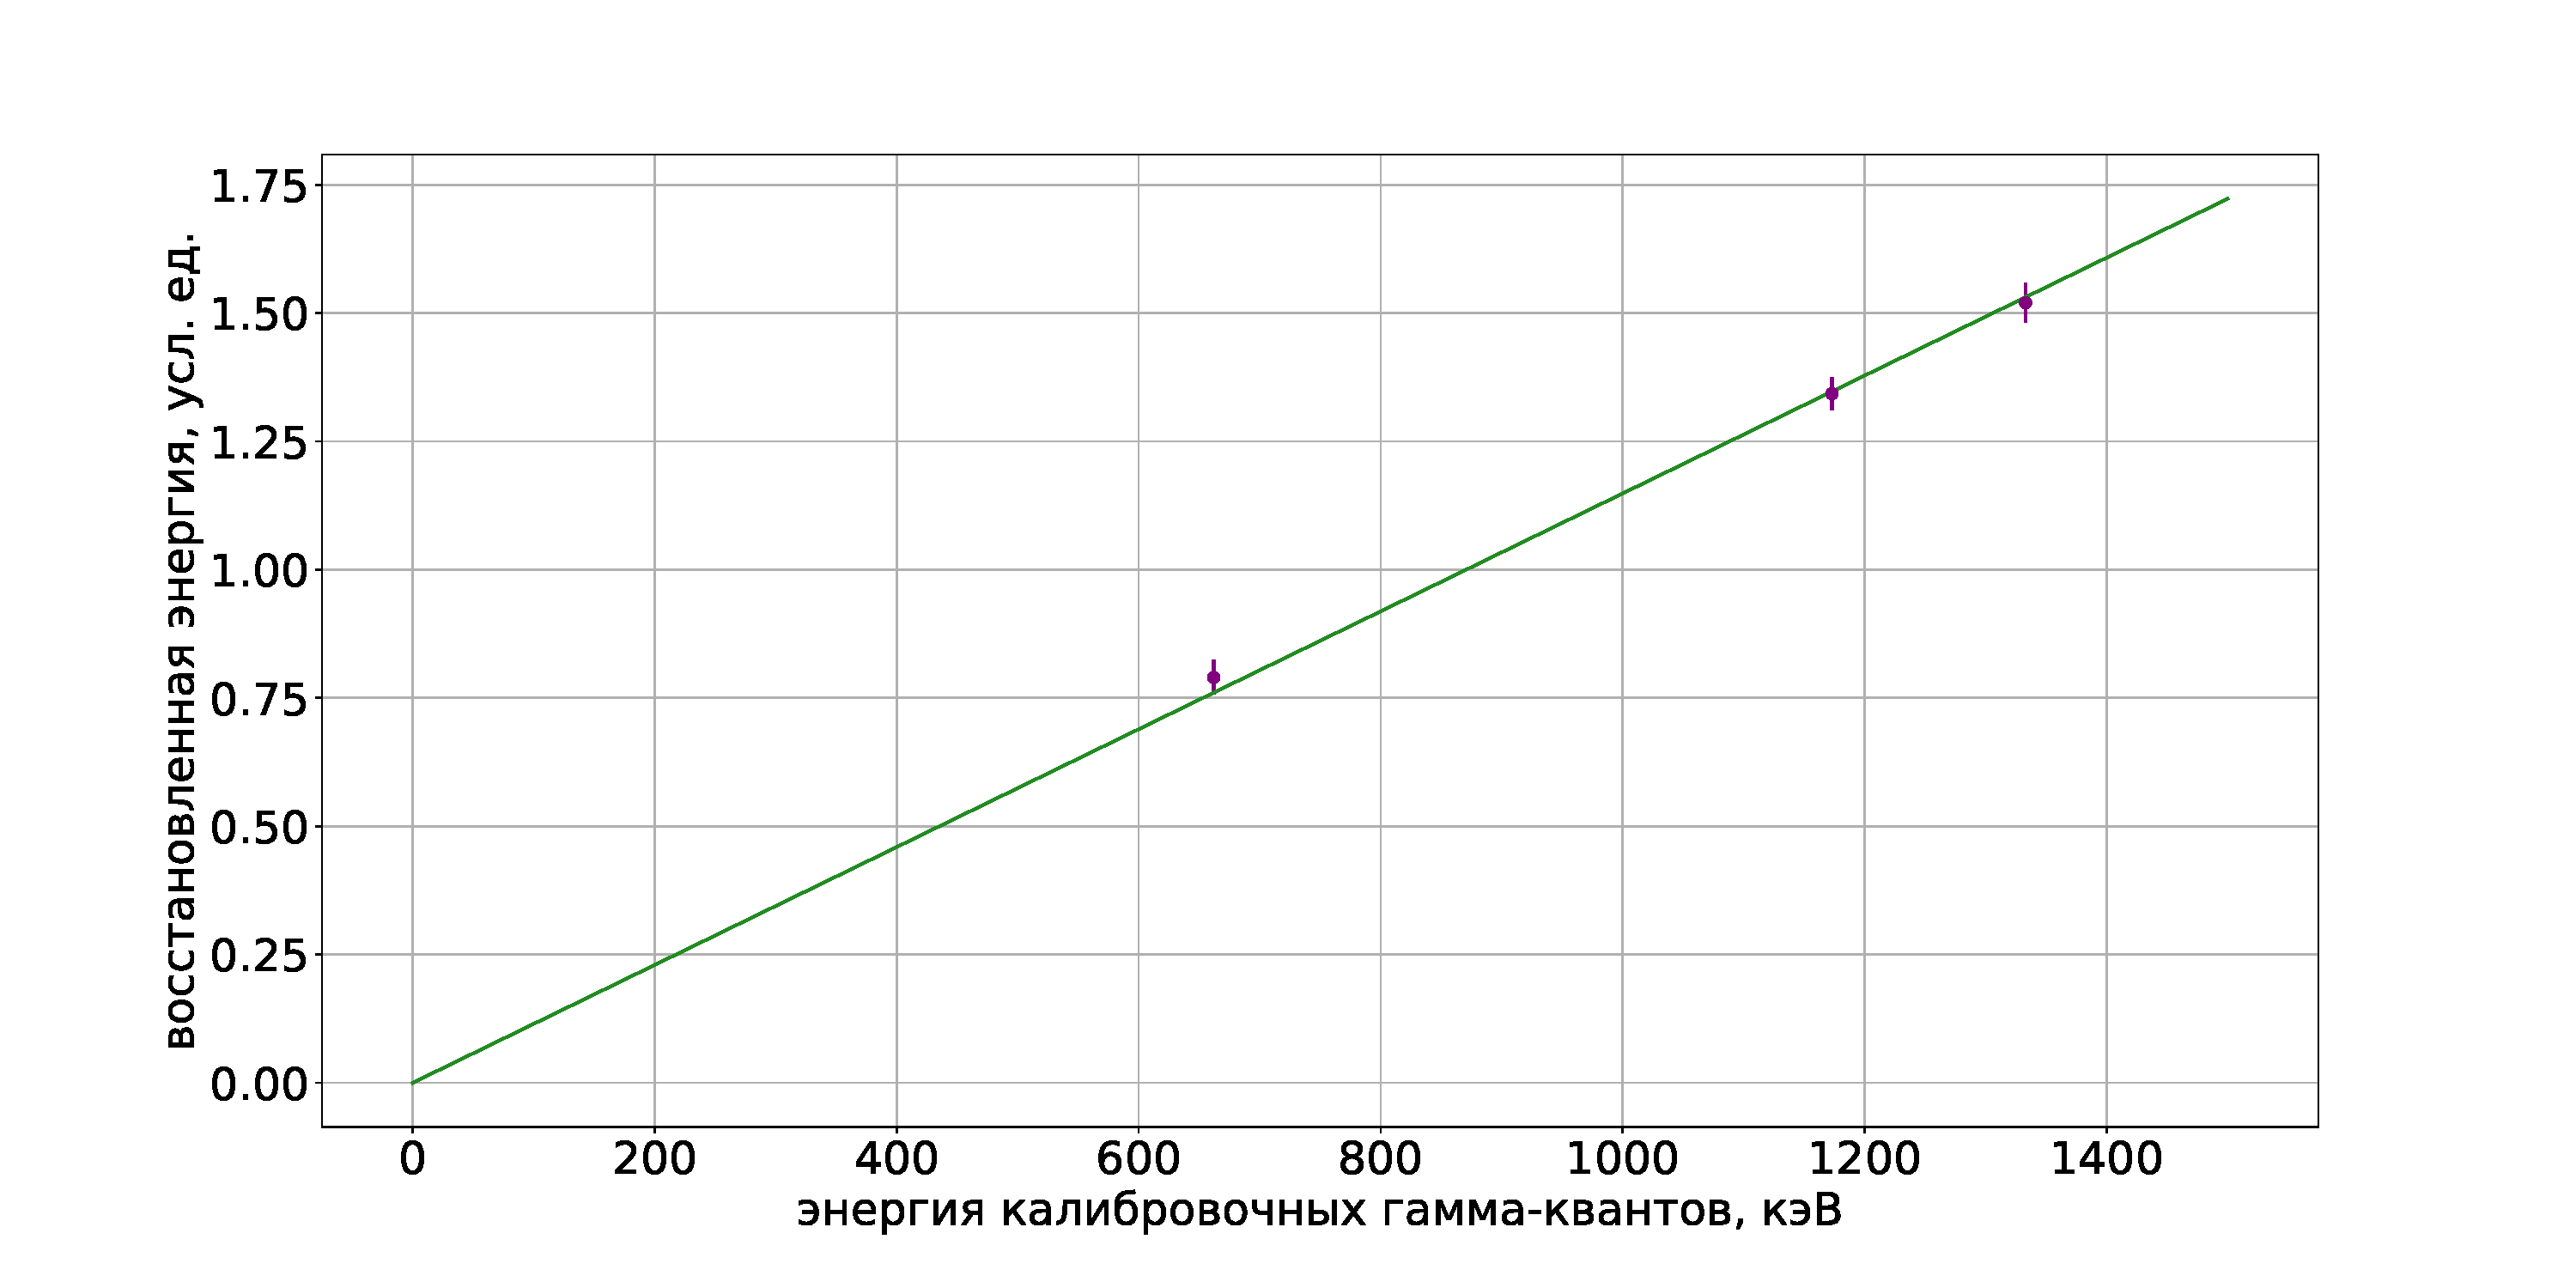
\includegraphics[width=1\linewidth]{images/calibr2022.pdf}}
  \caption{Калибровочный график для сеанса на КАЭС}
  \label{img:calibr2022}  
\end{figure}

\begin{table}[hbt]
    \centering
        \caption{Положения пиков и энергетическое разрешение (сеанс на КАЭС)}
\begin{tabular}{|c|c|c|c|}
\hline
    Энергия, кэВ & Положение пика, кэВ & ($\sigma/E$), \% & FWHM/E,  \%\\
    \hline
    662 & 688$\pm$29 & 8.4 & 19.6\\
    \hline
    1173 & 1169$\pm$27 & 3.7 & 8.7\\
    \hline
    1333 & 1323$\pm$33 & 3.9 & 9.2\\
    \hline
\end{tabular}    
\label{tab:resolution2022}
\end{table}


\section{SE-калибровки}
\label{sect3_4}

Сигналы от одиночных электронов ионизации представляют собой кластеры из равномерно распределенных по времени внутри кластера однофотоэлектронных импульсов. Как уже было упомянуто, SE-данные предсталяют собой формы сигналов в случайные моменты времени. Данные формы сигналов могут содержать как и искомые сигналы, так и совершенно разные события, а также случайные импульсы. Для отбора кластеров импульсов, соответствующих сигналам от одиночных электронов ионизации был применен следующий алгоритм:
\begin{enumerate}
    \itemОтбирались импульсы с амплитудой больше пороговой. Таблица с пороговыми значениями для сеанса на Калининской АЭС приведена в~\ref{AppendixA2}. Пороговые значения вычислялись как $\mu-2\sigma$, где $\mu$ и $\sigma$ -- параметры фита однофотоэлектронного спектра в соответствующем канале.
    \itemОтбирались такие последовательности импульсов, чтобы между любыми двумя из них расстояние было не больше $\Delta T$=500~нс. Величина $\Delta T$ подбиралась экспериментально исходя из знания о том, что длительность кластера, соответствующего электролюминесценции, составляет~$\approx$2~мкс. 
\end{enumerate}

Распределение SE-событий по длительности представлено на рисунке~\ref{img:seduration}. Как и во время сеанса на КАЭС, так и во время инженерного сеанса наблюдались события длительностью существенно меньшей, чем средняя длительность электролюминесценции. Данные события на графиках, представленных на рисунке~\ref{img:seduration}, составляют пик слева от основного. Такие "короткие" события возникают, если электролюминесценция происходит с самого края детектора, где электролюминесцентный зазор ограничен кольцом-держателем сетки. Для дальнейшего анализа данные события были отброшены. Границы отбора по длительности показаны на рисунке~\ref{img:seduration} красными линиями. Распределения суммарного светосбора по данным верхней матрицы для SE-данных представлены на рисунке~\ref{img:sespesp}.
\begin{figure}[H]
  \begin{minipage}[ht]{0.49\linewidth}    \center{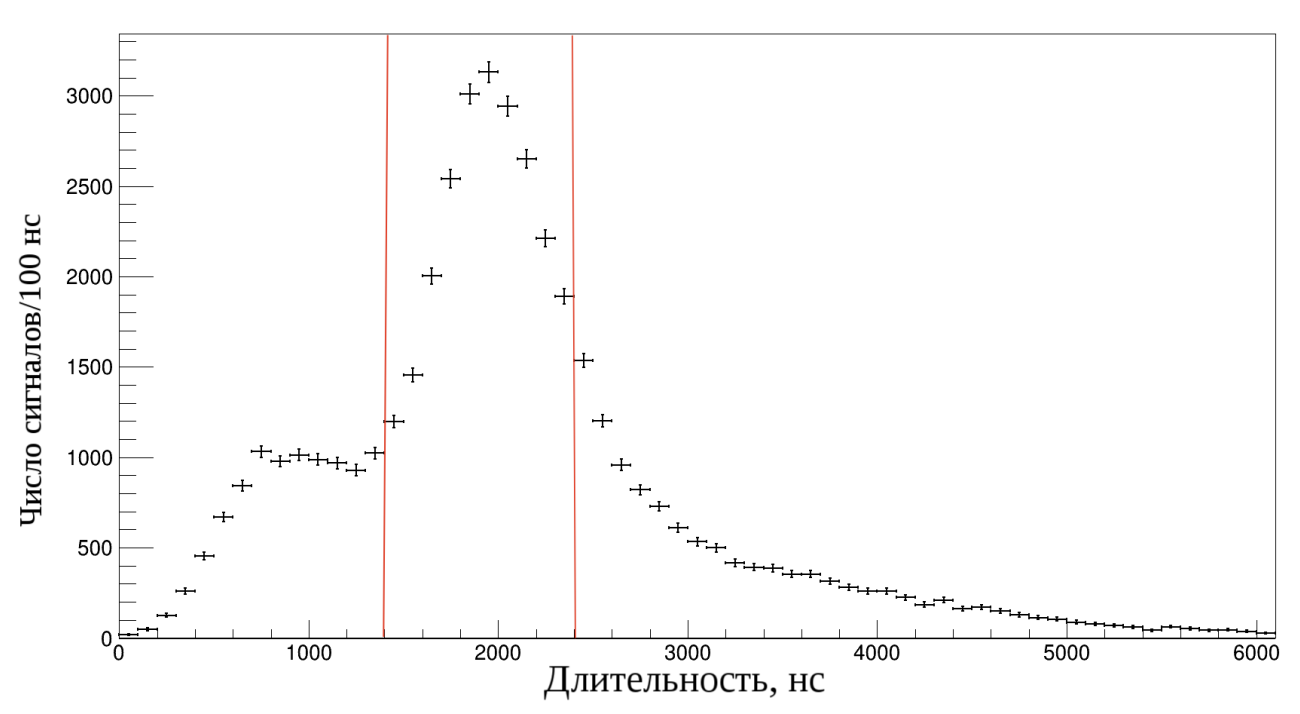
\includegraphics[width=1.0\linewidth]{images/seduration2019.png} \\ а)}
  \end{minipage}
  \hfill
  \begin{minipage}[ht]{0.49\linewidth}  \center{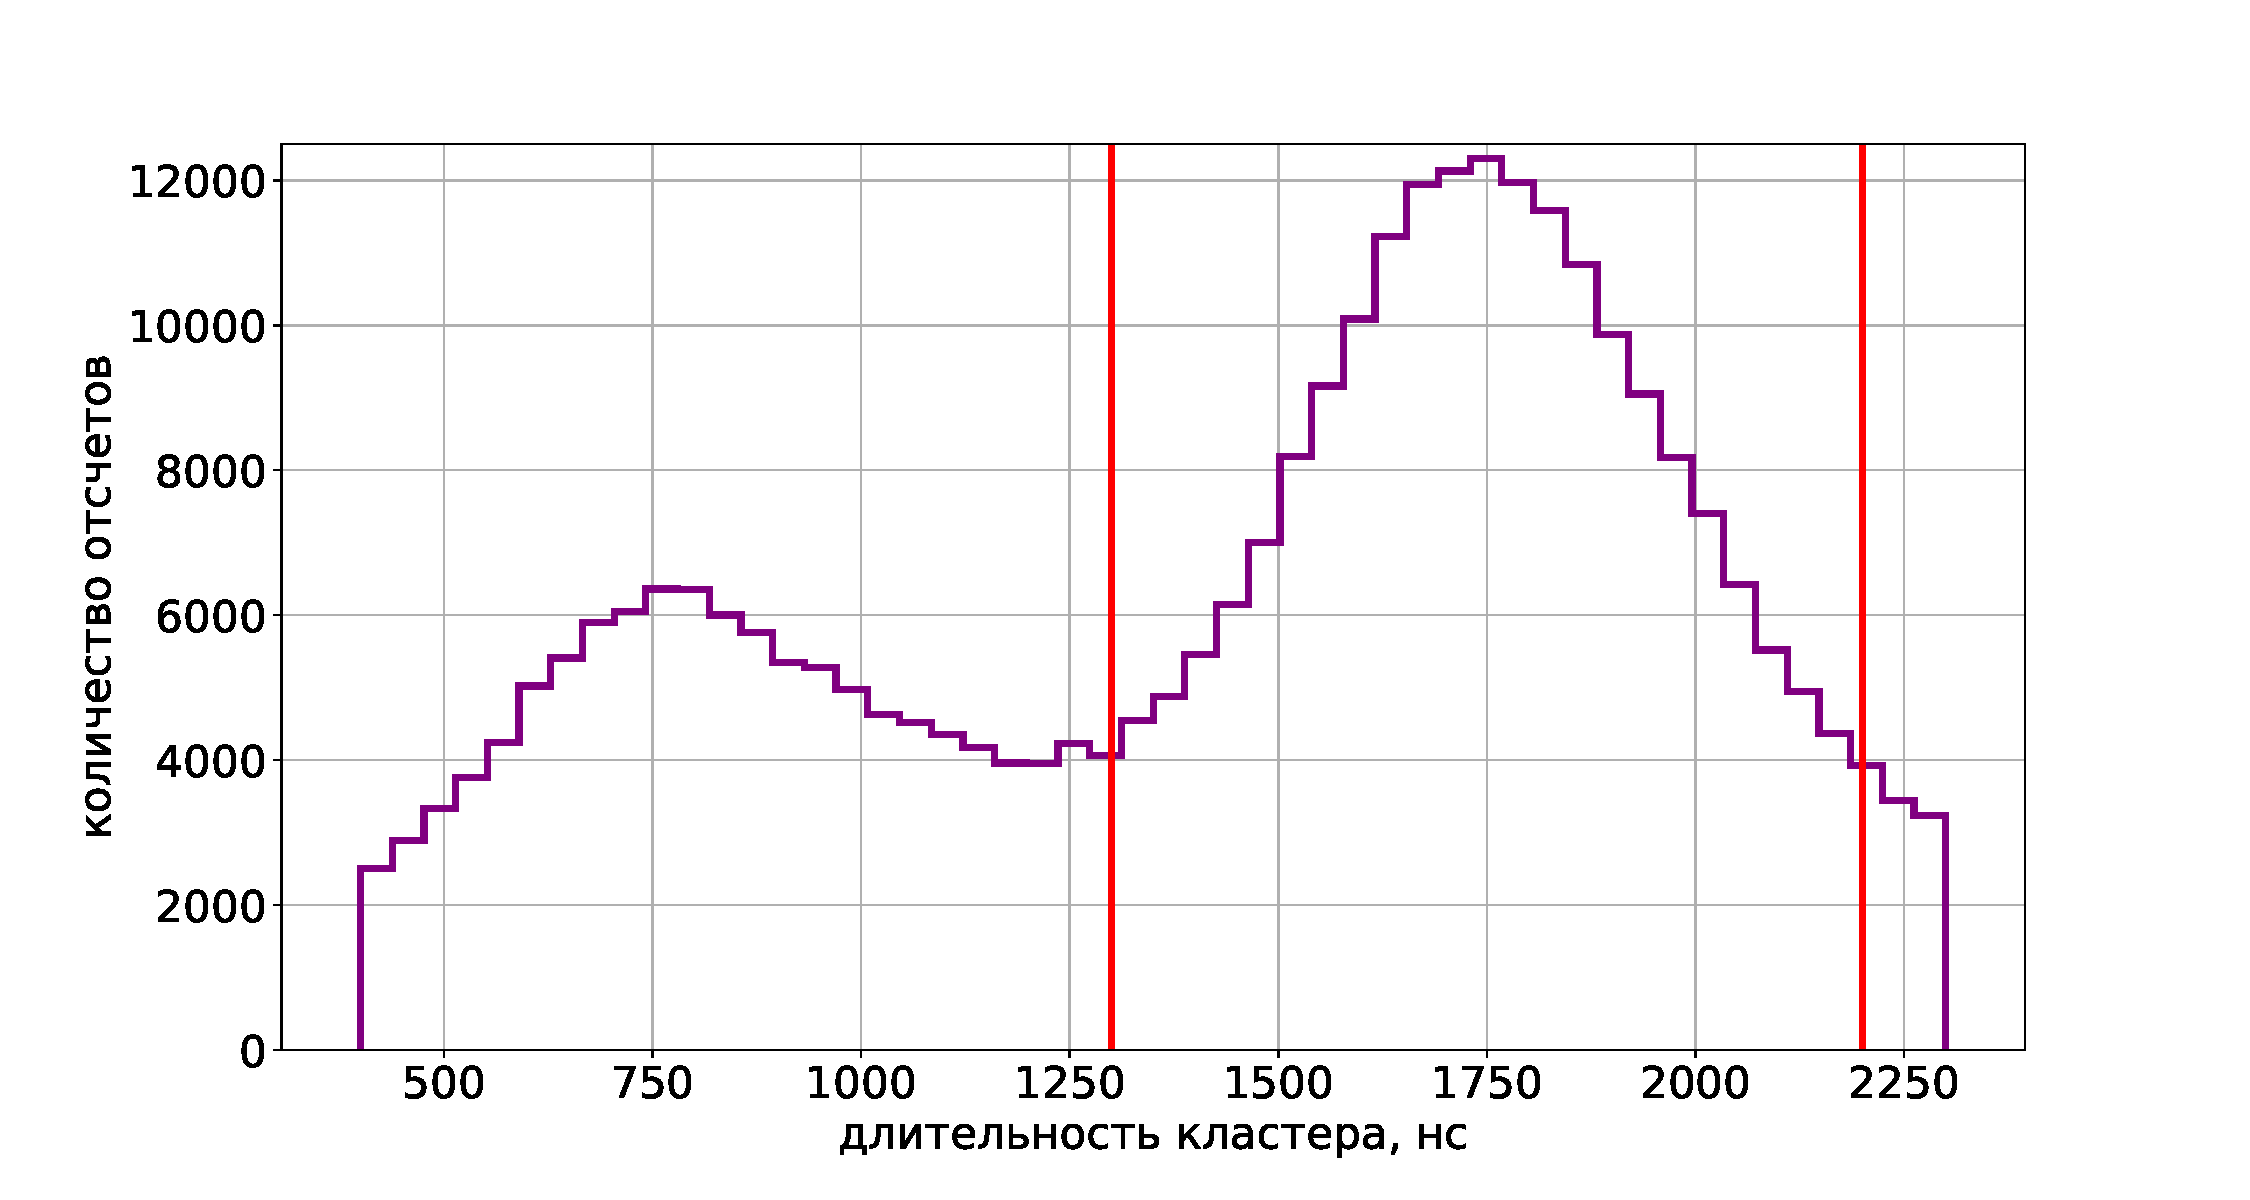
\includegraphics[width=1.0\linewidth]{images/seduration2022.pdf} \\ б)}
  \end{minipage}
  \caption{Распределение событий по длительности для инженерного сеанса (слева) и сеанса на КАЭС (справа)}
  \label{img:seduration}  
\end{figure}

\begin{figure}[H]
  \begin{minipage}[ht]{0.49\linewidth}    \center{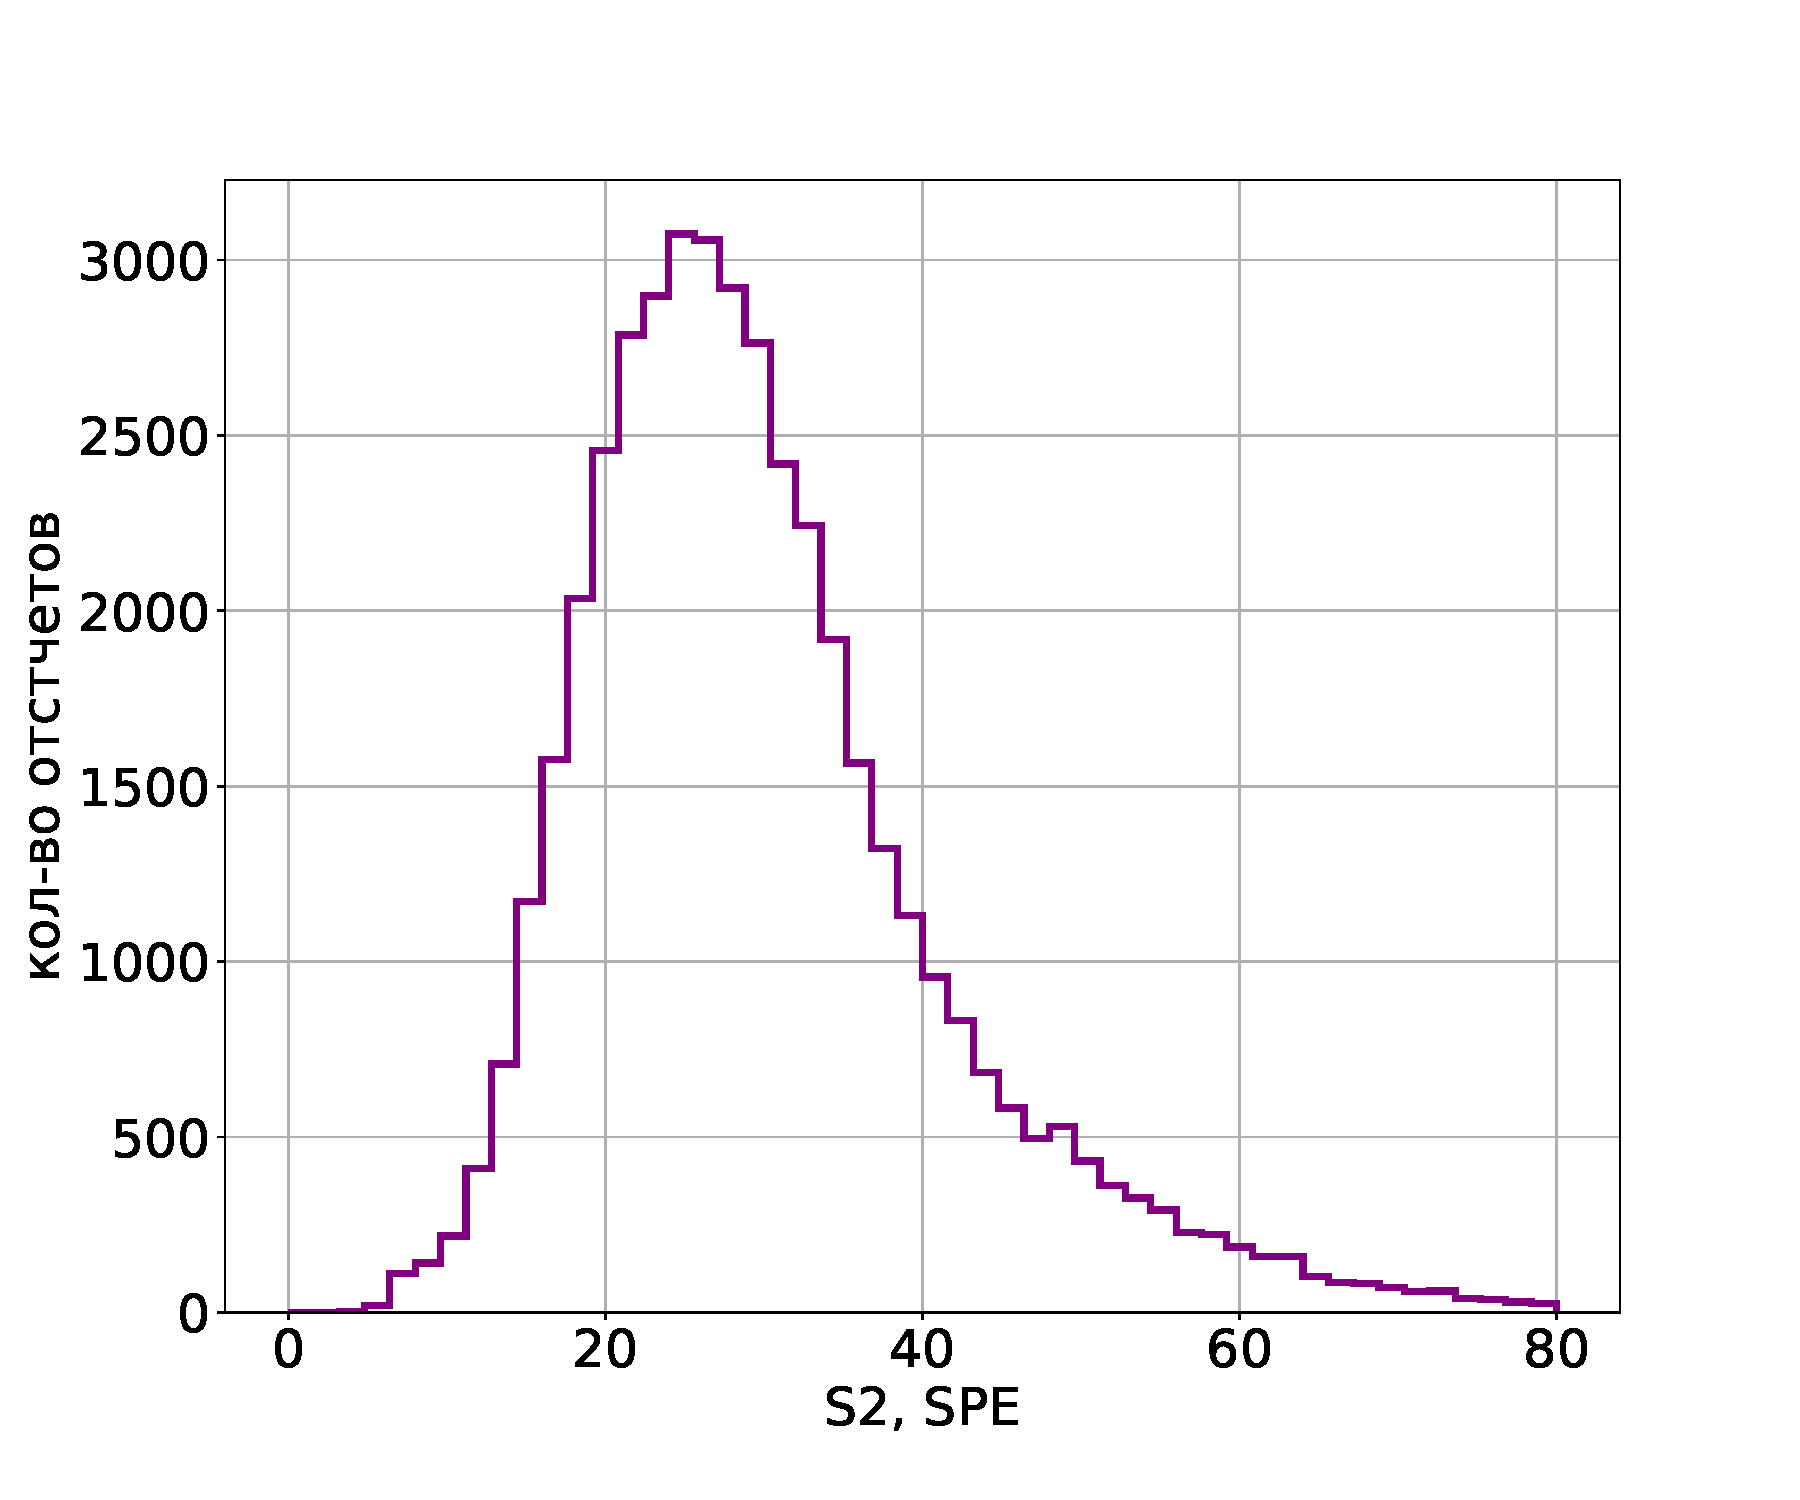
\includegraphics[width=1.0\linewidth]{images/se2019sp.pdf} \\ а)}
  \end{minipage}
  \hfill
  \begin{minipage}[ht]{0.49\linewidth}  \center{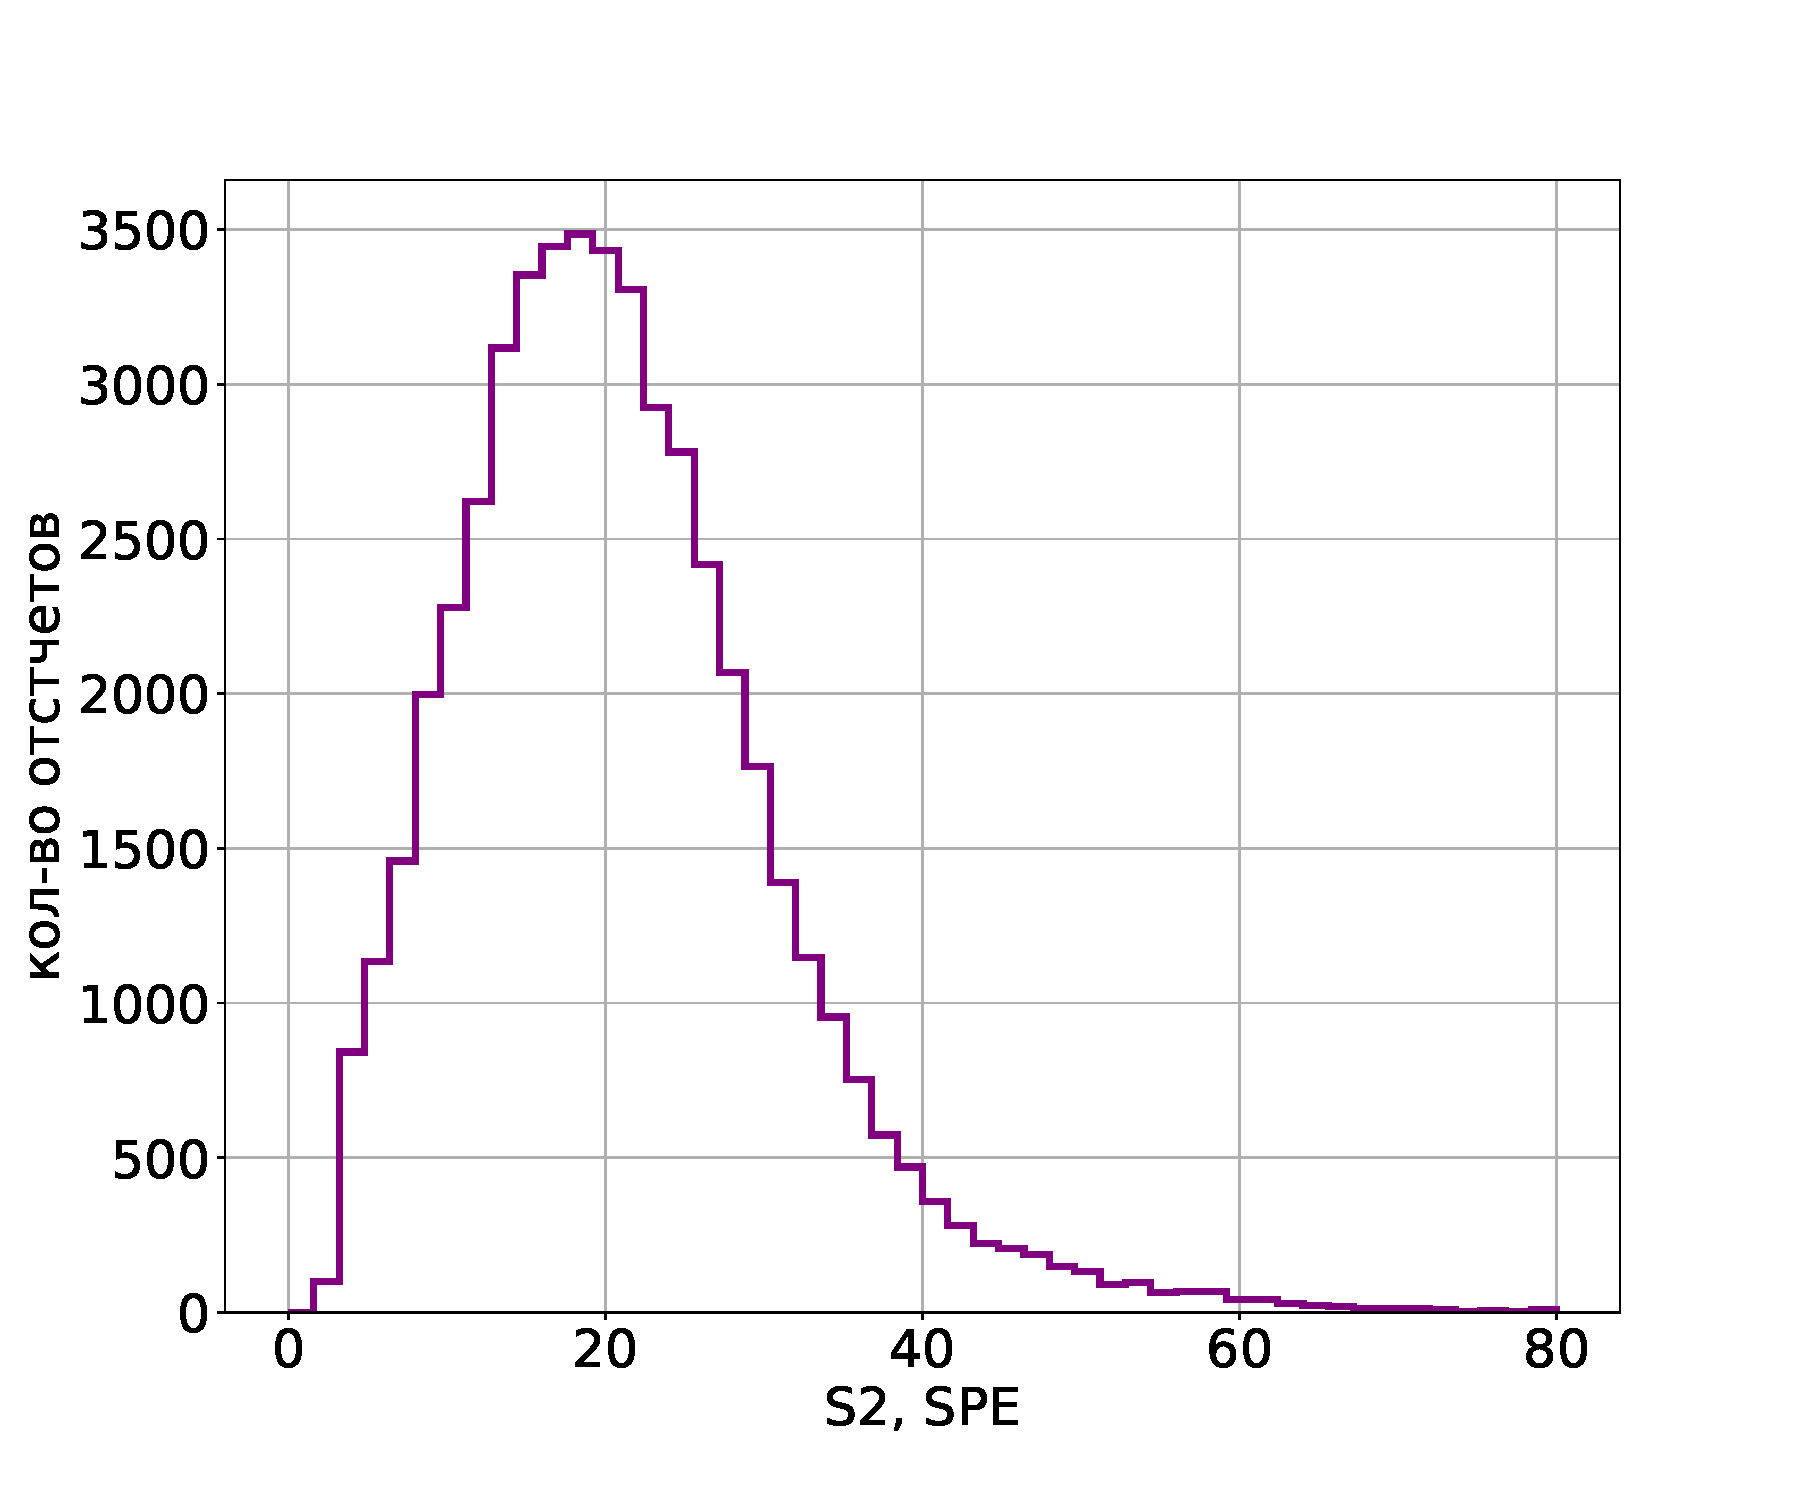
\includegraphics[width=1.0\linewidth]{images/se2022sp.pdf} \\ б)}
  \end{minipage}
  \caption{Распределения S2 в единицах SPE для SE-данных для инженерного сеанса (слева) и сеанса на КАЭС (справа)}
  \label{img:sespesp}  
\end{figure}

\section{Расчет ионизационного выхода и коэффициента экстракции электронов}
\label{sect3_5}
%Для расчета ионизационного выхода требуется величина сигнала от калибровочных гамм в единицах электронов ионизации.
Расчет ионизационного выхода (ionization yield -- IY) производился путем сравнения величины сигнала электролюминесценции от калибровочных гамма-источников и от одиночных электронов ионизации. Соответственно, для данной процедуры требуется выделение одиночного пика калибровочного гамма-источника. Так как разделение пиков $^{60}$Co возможно только в режиме антикорреляции, был использован пик меньшей энергии и данные SE сигналов. Значение ионизационного выхода рассчитывается по формуле:
%мб вместо IY использовать большую фигурную Q
\begin{equation}
    IY = \frac{A_{gamma\:source}}{A_{SE}\cdot E} \qquad \left[ \frac{e^-}{\text{кэВ}} \right]
    \label{formula:IY_calc},
\end{equation} где $A_{gamma\:source}$ и $A_{SE}$ -- положения пиков в фотоэлектронах после процедуры пространственного и энергетического восстановления, a $E$ -- энергия гамма-квантов соответствующего калибровочного источника. Однако, для малых сигналов требуется дополнительная коррекция площади SPE.
%для одиночных SPE для SPE формирующих большую электролюминесценцию имеются различия.
Дело в том, что в импульсах имеется низкоамплитудный хвост, который плохо учитывается в SE-данных, однако, очевидно, вносит вклад при расчете площади событий от калибровочных гамма-источников. Соответственно, требуется коррекция. Форма сигнала SPE для инженерного сеанса и сеанса на КАЭС совпадает, сравнение приведено на рисунке~\ref{img:spe_eff} а).

 Зависимость эффективности вычисления площади SE в зависимости от числа SPE в пачке приведена на рисунке~\ref{img:spe_eff} б). Для данного рассчета моделировались пачки фотоэлектронов с известным количество SPE в каждой и полученной в результате обработки значение количества SPE сравнивалось с изначальным. В связи с этим значение ионизационного выхода, рассчитанное по формуле ~\ref{formula:IY_calc} требуется умножить на соответствующий поправочный коэффициент:
\begin{equation}
    IY = k\cdot  \frac{A_{gamma\:source}}{A_{SE}\cdot E} \qquad \left[ \frac{e^-}{keV} \right]
    \label{formula:IY_calc_corr}
\end{equation}

Значения поправочного коэффициента: %как объяснить разницу если форма одинаковая? оффлайн менялся, и т.д.
\begin{itemize}
    \item ЛЭЯФ: $k = 0.80\pm 0.04$
    \item КАЭС: $k = 0.85\pm 0.03$
\end{itemize}

Значения отличаются для инженерного сеанса и для сеанса на КАЭС, так как были произведены некоторые изменения в параметрах отбора и интегрирования малых импульсов REDOffline.
\begin{figure}[ht]
  \begin{minipage}[ht]{0.49\linewidth}
    \center{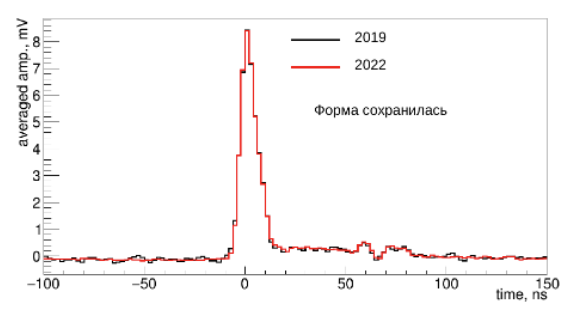
\includegraphics[width=1.0\linewidth]{images/SPE_shape.png} \\ а)}
  \end{minipage}
  \hfill
  \begin{minipage}[ht]{0.49\linewidth}
    \center{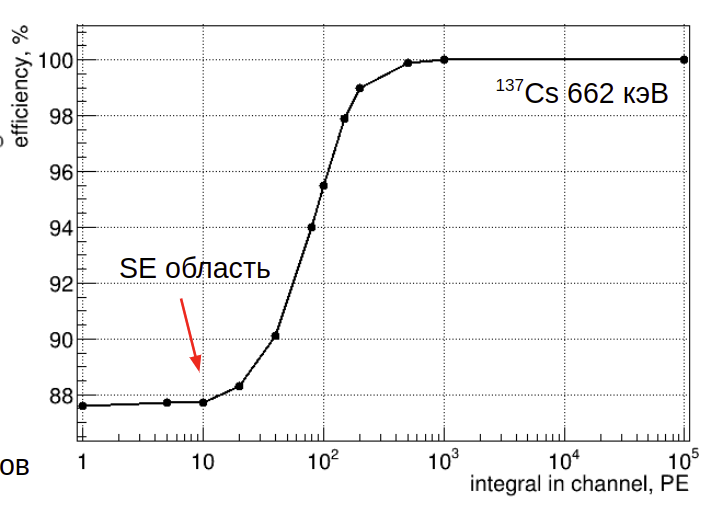
\includegraphics[width=1.0\linewidth]{images/SPE_efficiency.png} \\ б)}
  \end{minipage}
  \caption{а) Сравнение формы сигналов SPE для сеансов 2019 и 2022 гг. б) Зависимость эффективности вычисления площади импульса от количества SPE в импульсе.}
  \label{img:spe_eff}  
\end{figure}

В качестве калибровочного источника, пик от которого присутствует в расчетах, в ЛЭЯФ был использован $^{22}$Na c энергией гамма-квантов 511 кэВ, а при постановке эксперимента на КАЭС -- $^{137}$Cs с энергией гамма-квантов 662 кэВ. Так как расчет коэффициента экстракции электронов важен для предсказания спектра УКРН в детектор, на события был наложен дополнительный отбор на радиус от центра детектора (155 мм для инженерного сеанса и 130 мм для сеанса на КАЭС). Отбор событий, набранных во время сеанса на КАЭС совпадает с отбором, применявшимся для анализа УКРН-событий. Спектры S2 для гамма-калибровочных событий и для SE событий фитировались распределениями Гаусса для получения положений пиков. Калибровочные спектры на рисунке~\ref{img:NaCsfit}. SE спектры приведено на рисунке~\ref{img:SEfit}.

\begin{figure}[H]
  \begin{minipage}[ht]{0.49\linewidth}
    \center{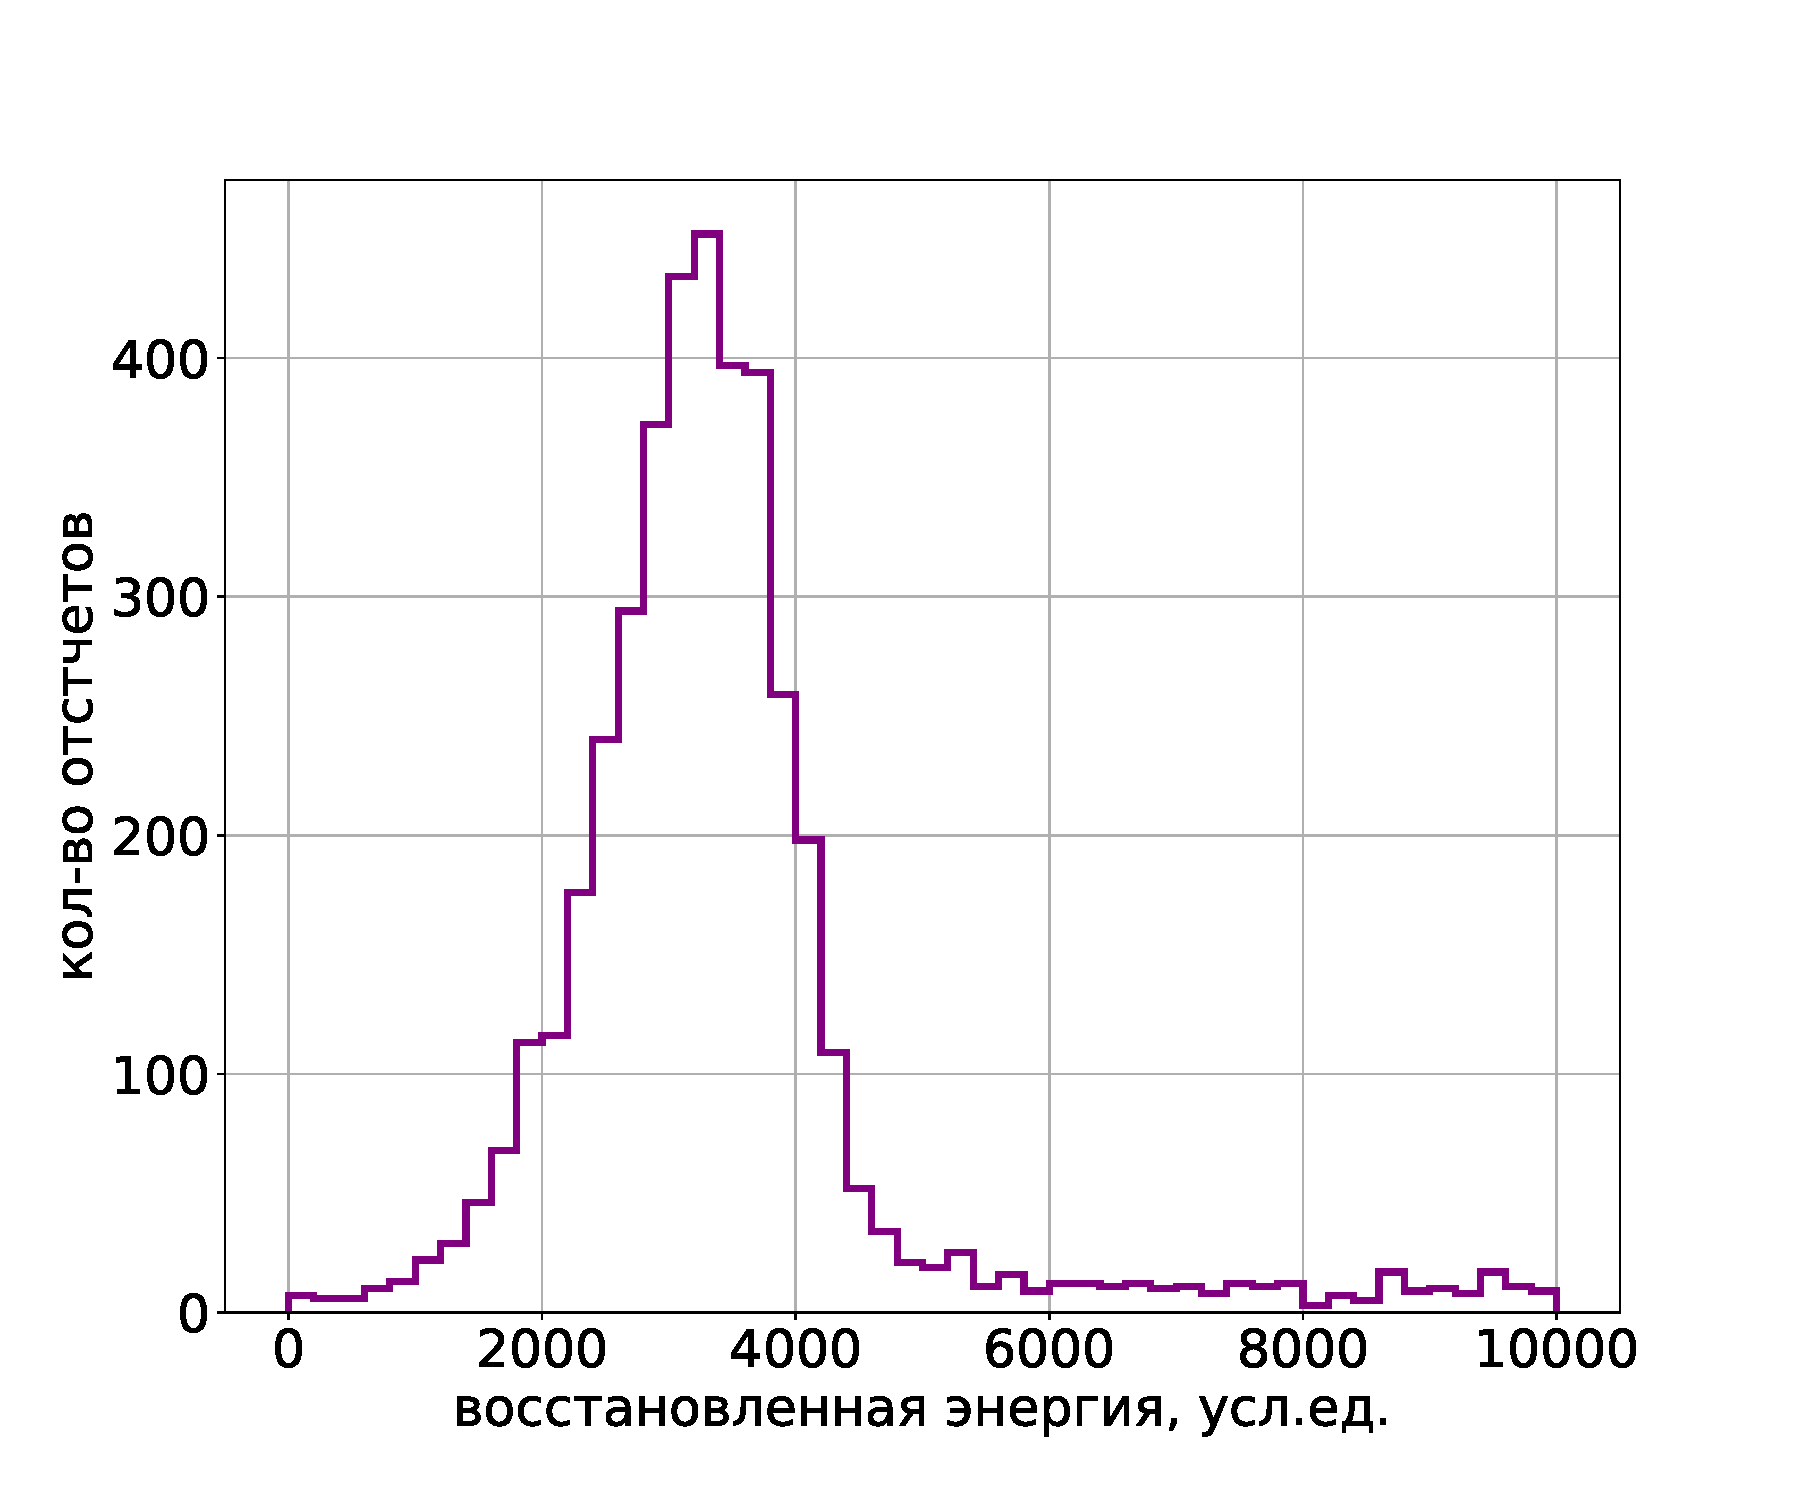
\includegraphics[width=1.0\linewidth]{images/na2019recsp.pdf} \\ а)}
  \end{minipage}
  \hfill
  \begin{minipage}[ht]{0.49\linewidth}
    \center{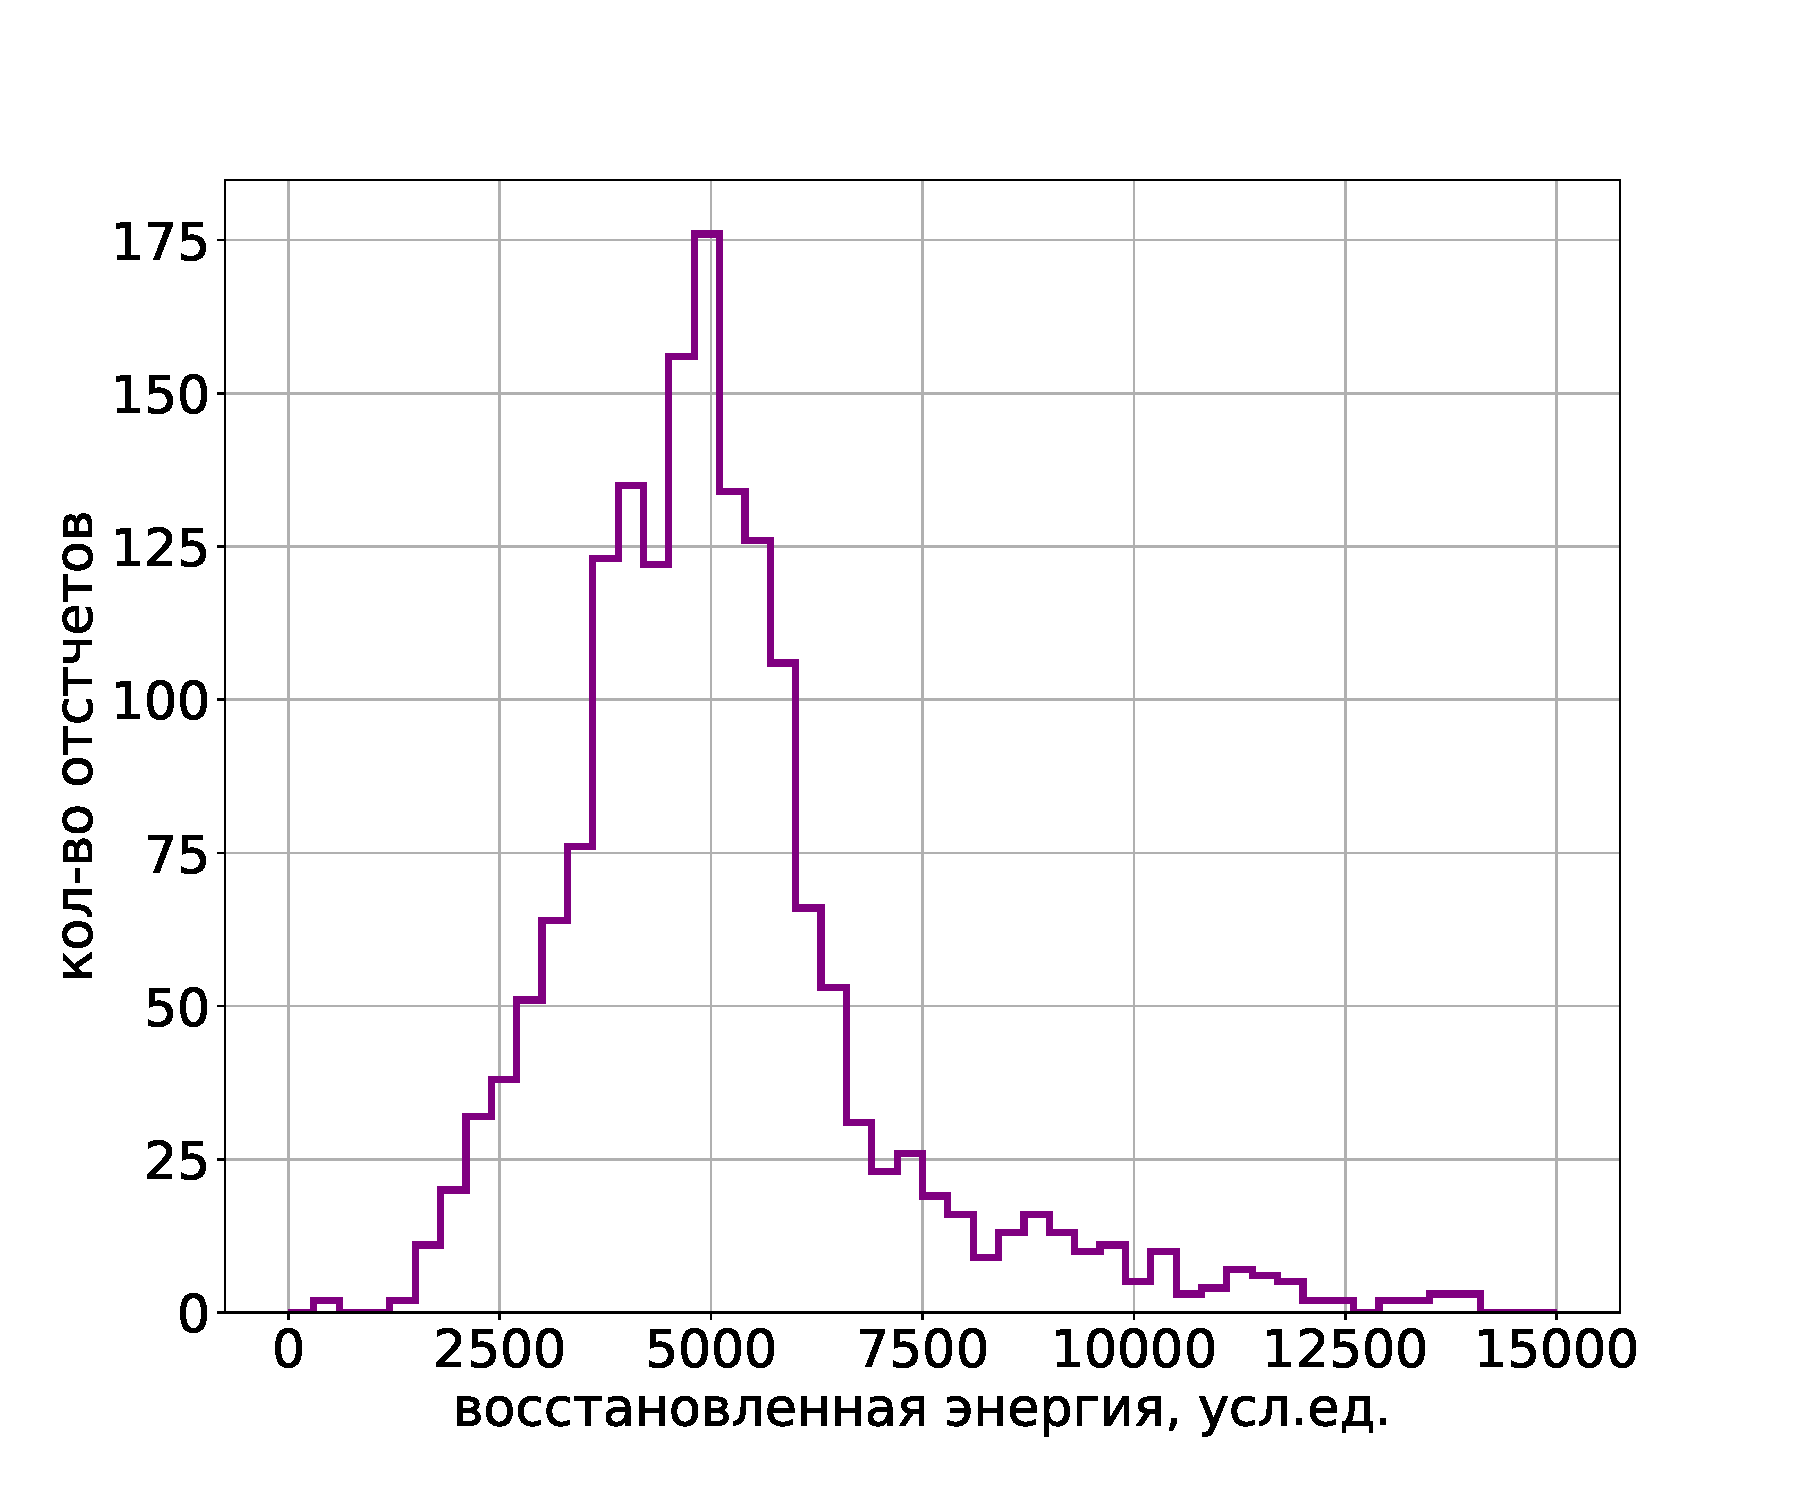
\includegraphics[width=1.0\linewidth]{images/cs2022recsp.pdf} \\ б)}
  \end{minipage}
  \caption[Спектры восстановленной энергии S2 для калибровочных источников]{а) Спектр восстановленной энергии S2 для $^{22}$Na (инженерный сеанс) б) Спектр восстановленной энергии S2 для $^{137}$Cs (сеанс на КАЭС)}
  \label{img:NaCsfit}  
\end{figure}

\begin{figure}[H]
  \begin{minipage}[ht]{0.49\linewidth}
    \center{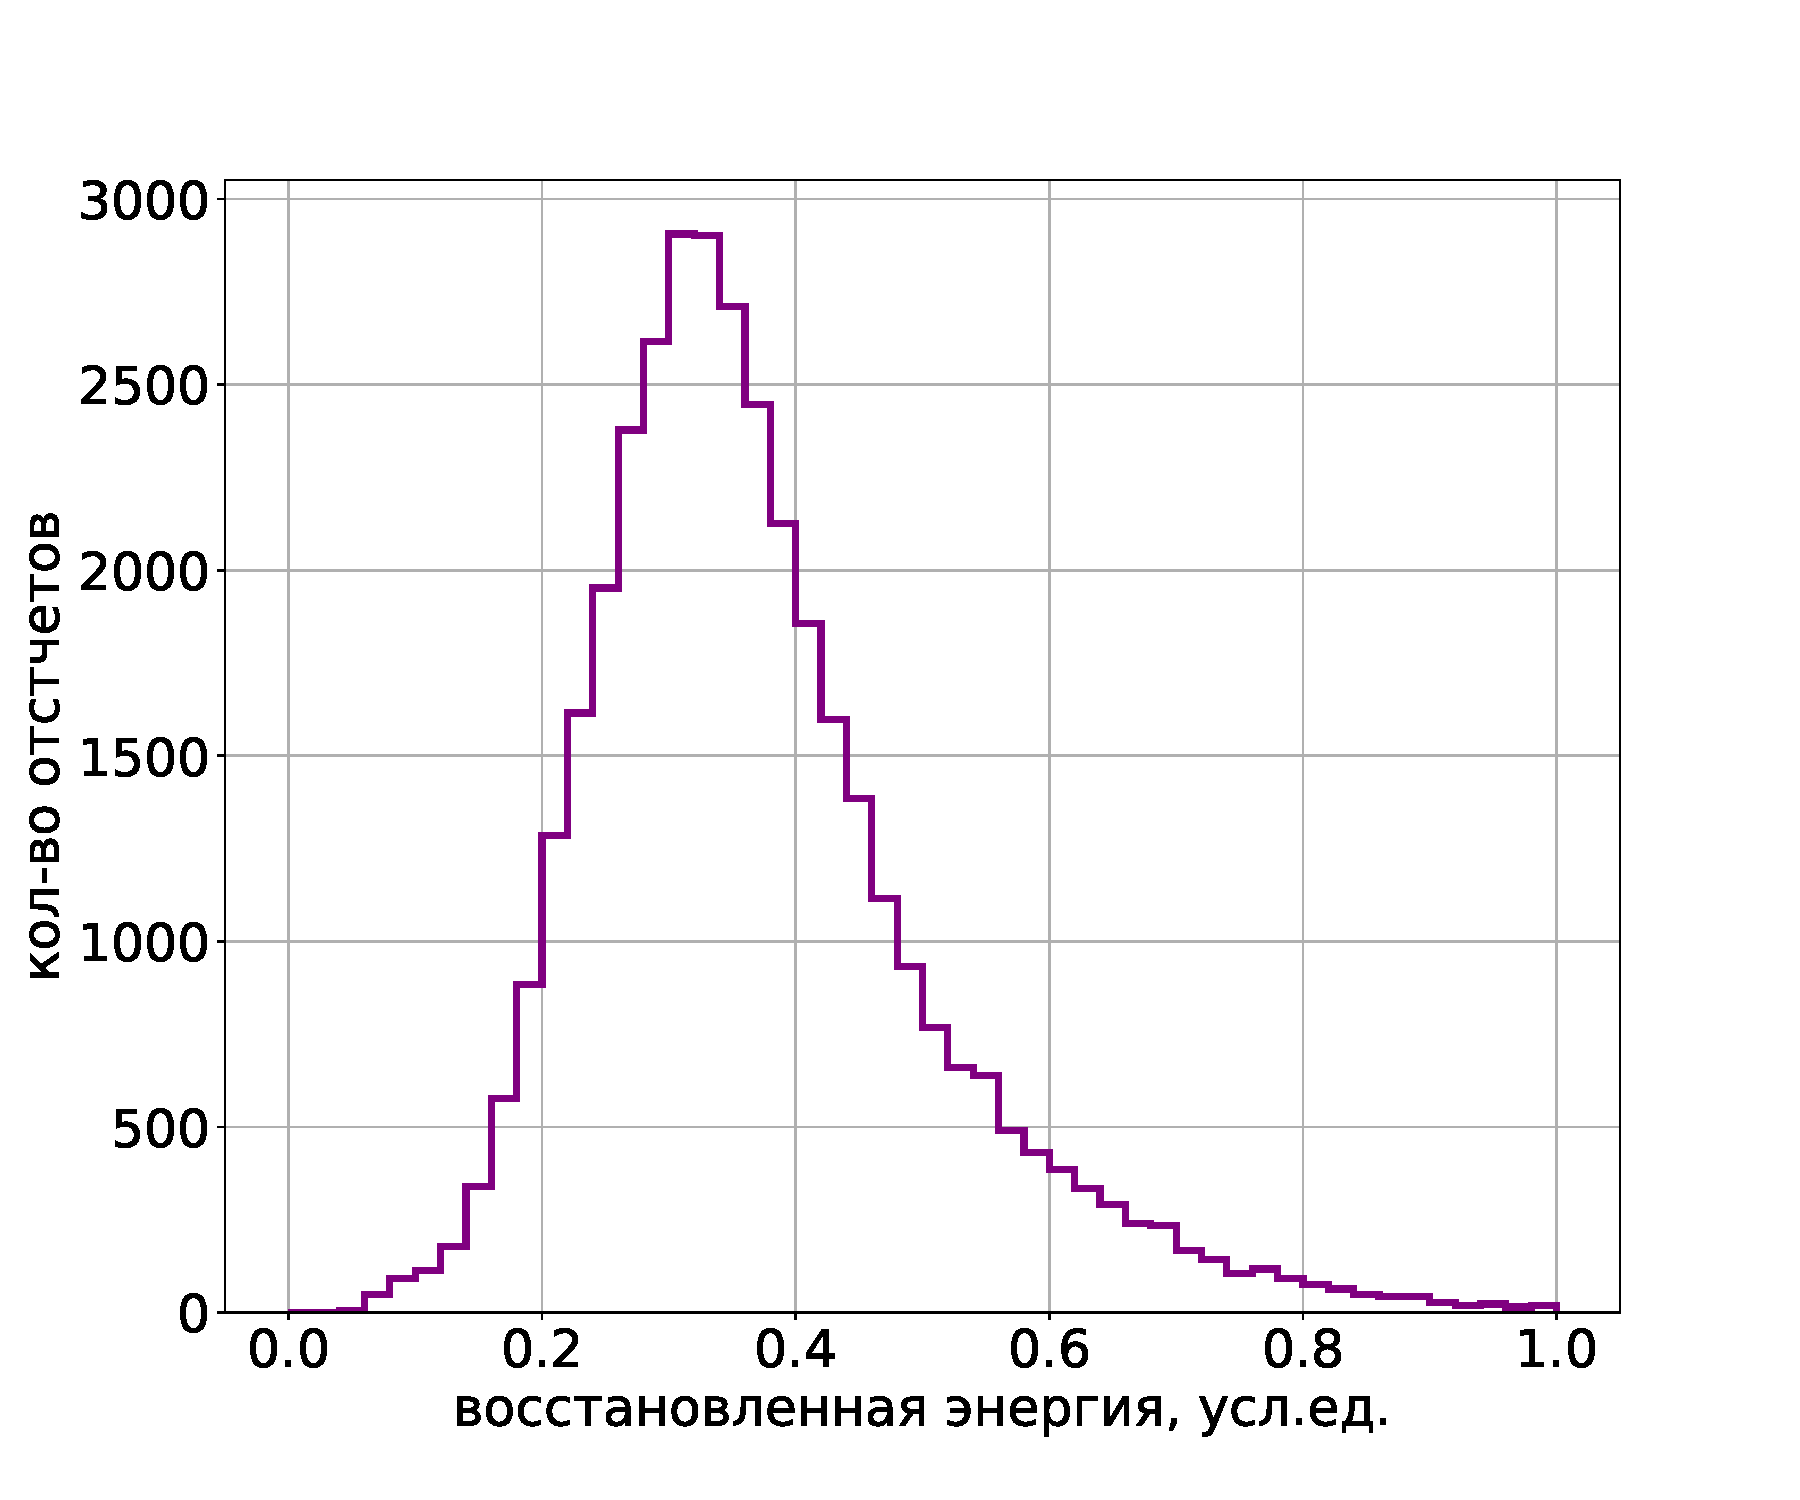
\includegraphics[width=1.0\linewidth]{images/se2019recsp.pdf} \\ а)}
  \end{minipage}
  \hfill
  \begin{minipage}[ht]{0.49\linewidth}
    \center{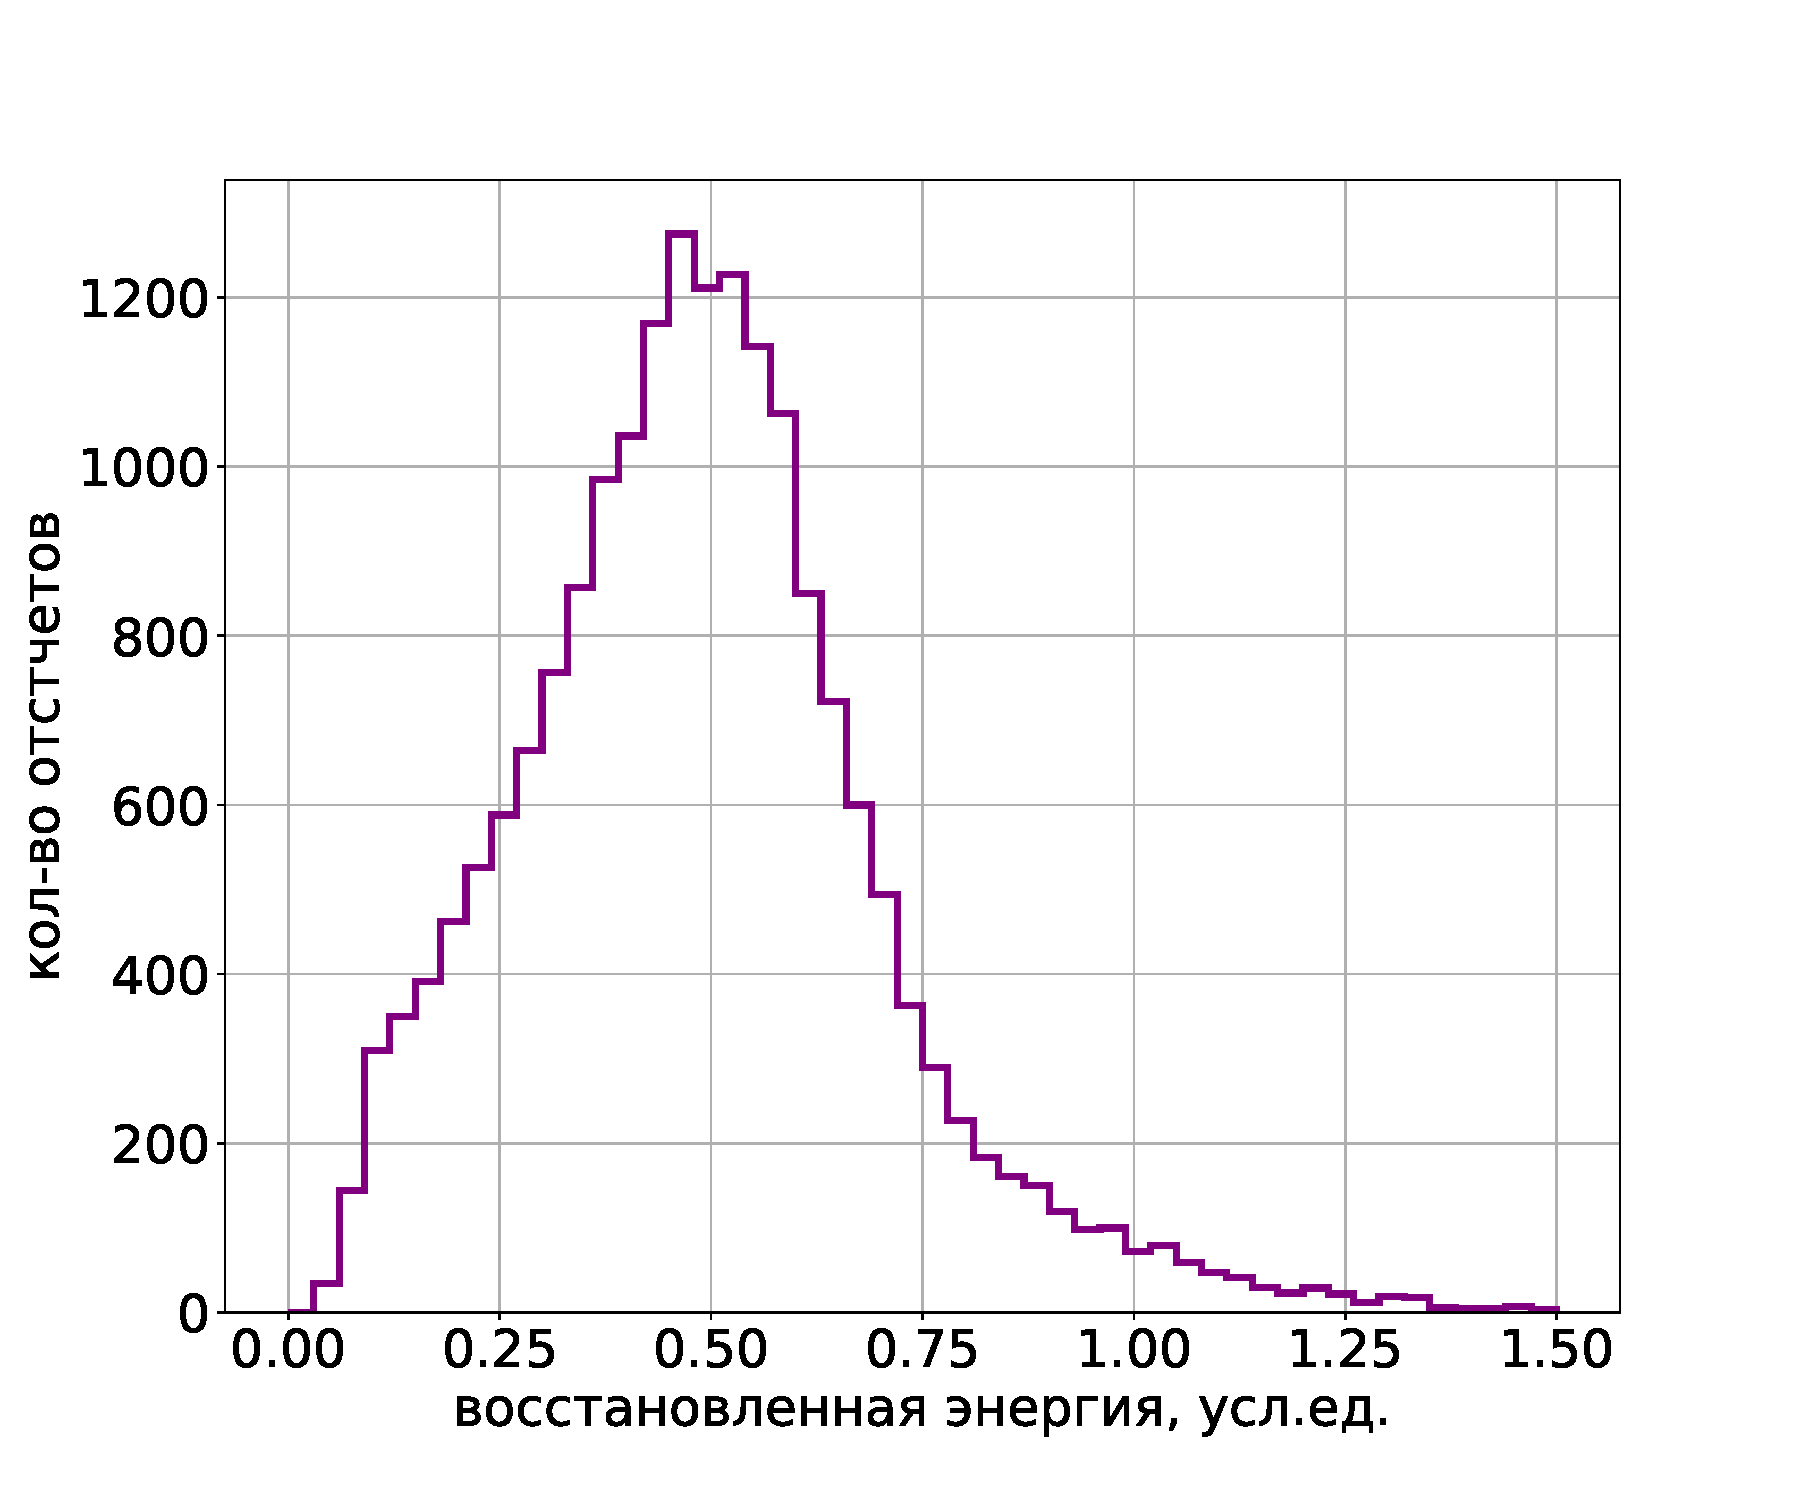
\includegraphics[width=1.0\linewidth]{images/se2022recsp.pdf} \\ б)}
  \end{minipage}
  \caption[спектры восстановленной энергии S2 для SE-данных]{а) Спектр восстановленной энергии S2 для SE (инженерный сеанс) б) Спектр восстановленной энергии S2 для SE (сеанс на КАЭС)}
  \label{img:SEfit}  
\end{figure}

\parОсновная идея рассчета коэффициента экстракции электронов состоит в сравнении количества рожденных электронов в месте взаимодействия гамма-кванта с веществом и количества зарегистрированных электронов ионизации по S2. 
Значения величин ионизации для соответствующих энергий, были рассчитаны с использованием программного пакета NEST %версия?. 
\parПолученные значения ионизационного выхода и коэффициента экстракции электронов:
\begin{itemize}
    \item 2019: IY = 15.6$\pm$0.7 e/keV, EEE = 38$\pm$6.1\%
    \item 2022: IY = 12.9$\pm$0.7 e/keV, EEE = 34$\pm$5.9\%
\end{itemize}

Было произведено сравнение полученных значений с измерениями других коллабораций~\cite{Gouschin1978,AprileEEE_2014,Edwards_2018,PhysRevD.99.103024}. Результаты представлены на рисунке \ref{img:EEEworld}. Также на данном рисунке представлен расчет с использованием программного пакета NEST. Результаты, полученные в эксперименте РЭД-100 имеют тенденцию к отличию в большую сторону от общемировых значений. Вероятно, это связано с недостаточной точностью при расчете электрических полей в электролюминесцентном зазоре.

\begin{figure}[H]
\center{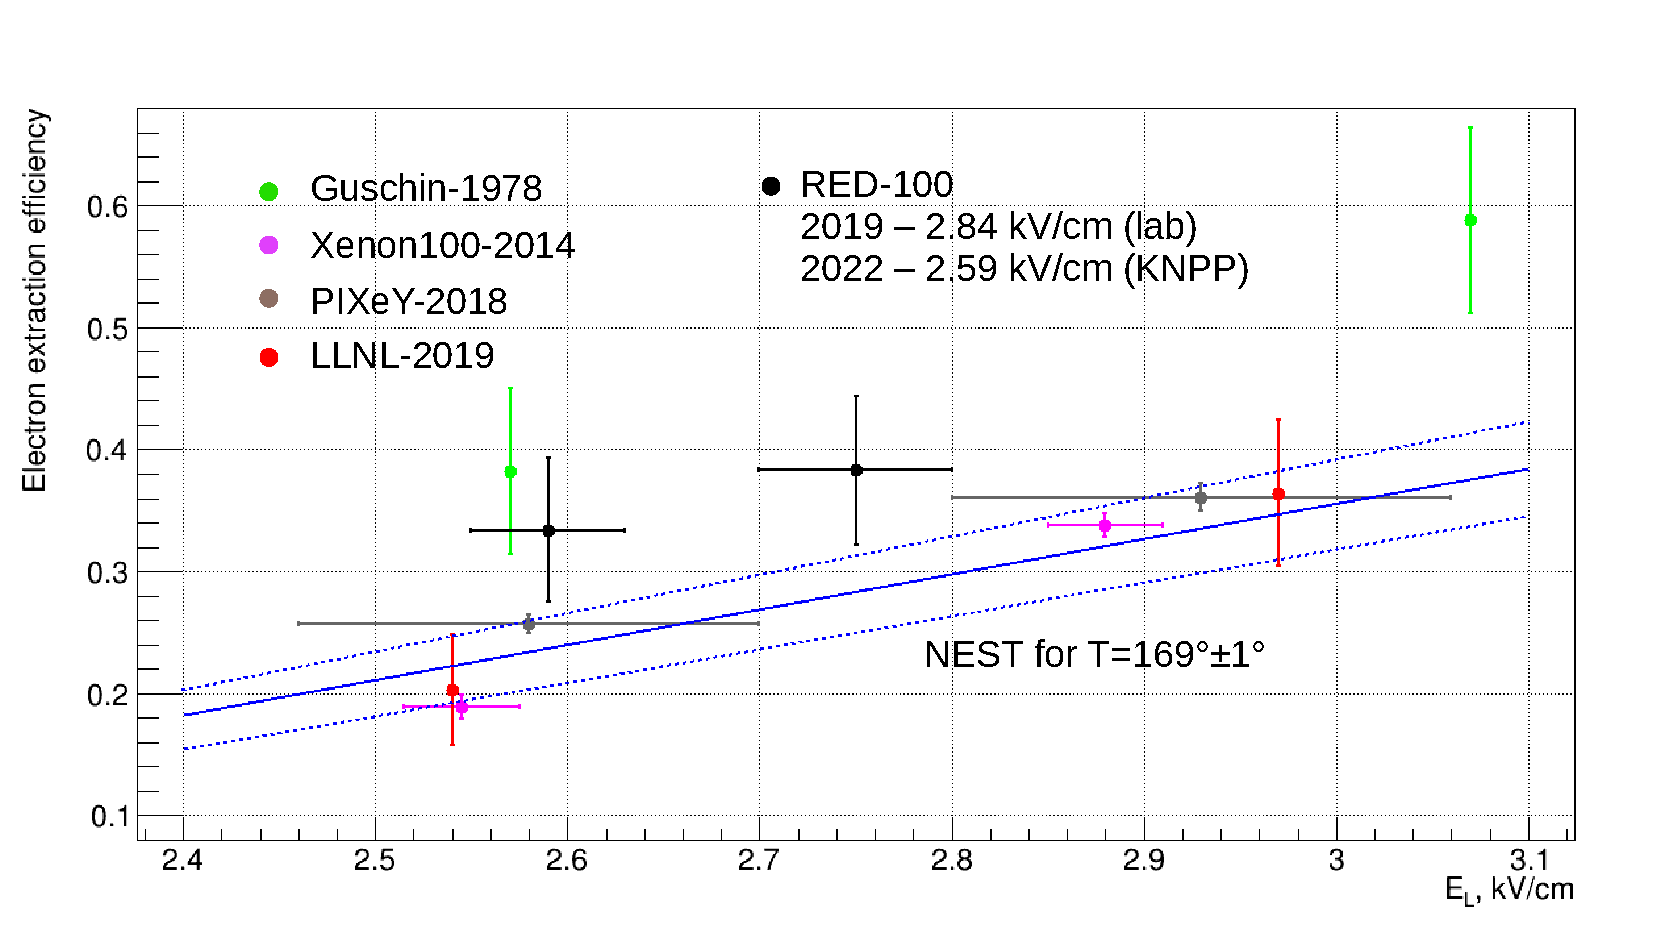
\includegraphics[width=1\linewidth]{images/RED_EEE_With_legend.pdf}}
  \caption{Сравнение результатов измерения ЕЕЕ в эксперименте РЭД-100 и другими коллаборациями, а также резульаты расчета данного коэффициента с использованием программного пакета NEST.}
  \label{img:EEEworld}  
\end{figure}